
\documentclass[
11pt,                          % standard font size
english                        % standard language
]{book}


%
% some macro packages
%

\usepackage[english]{babel}    % with explicit language
\usepackage{amsmath}           % ams mathematical stuff
\usepackage[utf8]{inputenc}    % smart input of funny chars
\usepackage[T1]{fontenc}       % also for the font encoding
\usepackage{longtable}         % tables longer than one page
\usepackage{exscale}           % large summation signs in 11pt
\usepackage[final]{graphicx}   % to include pdf pictures
\usepackage[sort]{cite}        % nicer citations
\usepackage{array}             % nice tables
\usepackage{wasysym}           % smiley symbols
\usepackage[a4paper]{geometry} % geometry of page layout
\usepackage{xspace}            % better spacing after macros
\usepackage{tikz}              % for commutative diagrams and stuff
\usepackage{chairx}            % the Chair X style file
\usepackage[expansion=false    % no font expansion
           ]{microtype}        % only protrusion
\usepackage[nottoc]{tocbibind} % refs and index in the toc
\usepackage[backref=page,      % backrefs in the bibliography
           final=true,         % always treat as final
           pdfpagelabels       % use pdf page labels
           ]{hyperref}         % hyperrefs are cool!
\usepackage[toc,page]{appendix}


%
% pdf files for graphics in the following directory:
%

\graphicspath{{../tikz/}}


%
% tikz libraries to be loaded, feel free to add more...
%

\usetikzlibrary{matrix}
\usetikzlibrary{arrows}
\usetikzlibrary{patterns}
\usetikzlibrary{decorations.pathreplacing}



%
% Specify which files wil be included 
% to have nicer aux-files
%

\includeonly{
  Introduction, 
  Chapter2, 
  Chapter3, 
  Chapter4, 
  Chapter5, 
  Chapter6,
  Chapter7,
  appendixA,
  appendixB,
  appendixC
  }


%
% page dimensions, scaling etc. Not final yet
%


\geometry{bindingoffset=1cm}
\geometry{hcentering=true}
\geometry{hscale=0.8}
\geometry{vscale=0.8}


%
% own local math macros follow here
%

\newcommand{\Eta}{\operatorname{H}}
\newcommand{\Rho}{\operatorname{P}}
\newcommand{\coproduct}{\Delta}
\newcommand{\ocoproduct}{\Delta}
\newcommand{\ostar}{\star}
\newcommand{\bch}[2]{\mathrm{BCH}\left(#1, #2\right)}
\newcommand{\bchpart}[3]{\mathrm{BCH}_{#1}\left(#2, #3\right)}
\newcommand{\bchparts}[4]{\mathrm{BCH}_{#1, #2}\left(#3, #4\right)}
\newcommand\ot[2]{\mathrel{\overset{\makebox[0pt]
	{\mbox{\normalfont\footnotesize\sffamily #1}}}{#2}}}

\newcount\colveccount
\newcommand*\colvec[1]{
        \global\colveccount#1
        \begin{pmatrix}
        \colvecnext
}
\def\colvecnext#1{
        #1
        \global\advance\colveccount-1
        \ifnum\colveccount>0
                \\
                \expandafter\colvecnext
        \else
                \end{pmatrix}
        \fi
}

%
% title page with the nice sign
% of the university and official stuff
%

\title{Convergence of the Gutt star product}
\author{Paul Stapor}

%
% the text starts here
%




\begin{document}

% ============================================================================
% 			Header part
% ============================================================================

% title page
%
\maketitle
\thispagestyle{empty}



% table of contents
%
\tableofcontents
\thispagestyle{empty}

% ============================================================================
% ////////////////////////////////////////////////////////////////////////////




% ============================================================================
% 			Main Part
% ============================================================================

% Introduction
%


%
% the Introduction of my master thesis
%

\chapter{Introduction}
\label{sec:Intro}

Here will be things like thanks to and so on...




% Chapter 2
%


%
% Chapter 2 of my master thesis:
% Still quiete a lot introductory
%

\chapter{Deformation quantization}

The starting point for every theory of quantization is surely mechanics. Here, 
mechanics means both, the classical and the quantum theory. Since we want to 
explain how one can link them together, we will give a short overview of both 
theories and show their similarities and their differences in the first section 
of this chapter. Then we will come to different aspects of quantization and 
state the most important ideas in the next part. In section three, we will 
focus on Deformation quantization and give an overview of this rather young 
theory.



\section{Mechanics: The Classical and the Quantum World}
\label{sec:chap2_Mechanics}

\subsection{Classical Mechanical Systems}
\label{subsec:chap2_Classical}
We want to recall briefly the notions of classical mechanics. There are many 
good books on this subject and also the notation is mostly uniform everywhere, 
but nevertheless want to refer to the books of Marsden and Ratiu 
\cite{marsden.ratiu:1999a} and Arnold \cite{arnold:1989a}, which give very good 
introductions and overviews of the whole theory.
Imagine the simplest model for a mechanical system, which is not trivial: a 
single particle with mass $m$ in $\mathbb{R}^3$ in a scalar potential $V$. We 
will denote his position by $q = (q^1, q^2, q^3) \in Q = \mathbb{R}^3$ and call 
the set of all possible positions $Q$ the configuration space. Since we also 
have a time coordinate $t \in \mathbb{R}$, we can describe the path on which 
the particle moves by $q(t)$. The state of the particle is completely described 
by its position and its velocity $(q(t), \dot q(t))$ and the velocity should be 
understood as a tangent vector $\dot q(t) \in T_{q(t)}Q = \mathbb{R}^3$. 
Therefore, the tangent bundle $TQ$, which is in this case $\mathbb{R}^6$, is 
sometimes called the state space. In classical mechanics, we can describe the 
movement of the particle with the Euler-Lagrange equations, which are derived 
from the Lagrange function by a variational principle. The Lagrange function of 
this system reads
\begin{equation*}
	\mathcal{L}(q, \dot q)
	=
	T(q, \dot q) - V(q, \dot q)
\end{equation*}
and $T(q, \dot q) = \frac{1}{2} m  \sum_{i=1}^3 \dot{q^i}^2$ is the kinetic 
energy. The action 
is defined as the integral
\begin{equation*}
	\mathcal{S}(q, \dot q)
	=
	\int\limits_{t_0}^{t_1}
	\mathcal{L}(q, \dot q)
	dt.
\end{equation*}
It is a physical observation, similar to a mathematical axiom, that this action 
functional is minimized along the trajectories of the particle. So fixing a 
starting point $q_0$ and an end point $q_1$ of a trajectory, we find
\begin{equation*}
	\delta \mathcal{S}
	\at{q(t_0) = q_0, q(t_1) = q_1}
	=
	0.
\end{equation*}
From this, one finds the Euler-Lagrange equations for $i = 1, 2, 3$
\begin{equation*}
	\frac{d}{dt} 
	\frac{\partial \mathcal{L}}{\partial \dot q^i}
	-
	\frac{\partial \mathcal{L}}{\partial q^i}
	=
	0.
\end{equation*}
In our case this means
\begin{equation*}
	\frac{d}{dt} 
	\frac{\partial T}{\partial \dot q^i}
	-
	\frac{\partial V}{\partial q^i}
	=
	m \ddot q
	-
	\frac{\partial V}{\partial q^i}
	=
	0
\end{equation*}
and we can integrate the equations to get the trajectory. So far, we described 
the system in the state space and for obvious reasons, this formalism is called 
the Lagrange formalism. It is not the only formalism, which describes to 
behaviour of the system: one can go to the so called Hamilton formalism, which 
is based on the conjugate momenta $p = (p_1, p_2, p_3) \in T_{q(t)}^*Q$
\begin{equation*}
	p_i(t)
	=
	\frac{\partial \mathcal{L}}{\partial \dot q^i}
\end{equation*}
and linked to the Lagrange formalism by a Legendre transformation. Now we can 
define the Hamilton function
\begin{equation*}
	H(q, p)
	=
	p_i q^i
	-
	\mathcal{L}(q, \dot q),
\end{equation*} 
which is the crucial quantity in this setting. It represents the energy of the 
system. On finds the equations
\begin{equation*}
	\frac{\partial H}{\partial p_i}
	=
	\frac{d q^i}{dt}
	\quad \text{ and } \quad
	- \frac{\partial H}{\partial q^i}
	=
	\frac{d p_i}{dt}.
\end{equation*}
They remind strongly of a symplectic structure and indeed this is the case: 
using the standard sympectic matrix
\begin{equation*}
	\omega
	=
	\begin{pmatrix}
		0 & \Unit
		\\
		- \Unit & 0
	\end{pmatrix}
\end{equation*}
one finds
\begin{equation*}
	\frac{d}{dt} \vector{q^i}{p_i}
	=
	\omega
	\vector{\frac{\partial H}{\partial q^i}}
	{\frac{\partial H}{\partial p_i}}.
\end{equation*}
More generally, one can define the Poisson bracket $\{f, g\}$ for two functions 
$\Cinfty(T^*Q)$ by
\begin{equation*}
	\{f, g\}
	=
	\sum\limits_{i=1}^3
	\left(
		\frac{\partial f}{\partial q^i}
		\frac{\partial g}{\partial p_i}
		-
		\frac{\partial f}{\partial p_i}
		\frac{\partial g}{\partial q^i}
	\right)
\end{equation*}
and finds the time evolution of a function $f$ given by
\begin{equation*}
	\frac{d}{dt} f
	=
	\{ f, H \}.
\end{equation*}
All of those objects have, of course, a geometrical interpretation which remain 
true for and allow generalizations from this very easy example. For a more 
complex system than one particle in a scalar potential, the configuration space 
$Q$ will be a smooth manifold, the state space $TQ$ is described by the tangent 
bundle and the phase space $T^*Q$ by the cotangent bundle. The transition from 
the Lagrange to the Hamilton formalism is done by a fiber derivative, the 
kinetic energy has a mathematical interpretation as a Riemannian metric and the 
Poisson bracket is the one which is due to the canonical symplectic form on the 
cotangent bundle. So in some sense, classical mechanics can be described by 
symplectic geometry.


The last conclusion, however, was a bit too fast. There are mechanical systems 
like the rigid body, which can not be described in the symplectic formalism, 
or which have certain symmetries and therefore allow a \emph{reduction}. A 
symmetry can mathematically be described by a Lie group $G$, which acts on 
$T^*Q$ and a reduction by a momentum map $J \colon T^*Q \longrightarrow 
\lie{g}^*$, where $\lie{g}$ is the Lie algebra of the Lie group and $\lie{g}^*$ 
its dual. The reduced phase space is a quotient of the cotangent bundle and 
does not need to be symplectic any more. Anyway, in both cases, the result will 
be something more general than a symplectic manifold: it will be a Poisson 
manifold. 
\begin{definition}[Poisson Manifold]
	A Poisson manifold is a tuple $(M, \{ \cdot, \cdot \})$ of a smooth 
	manifold $M$ and a Poisson bracket $\{ \cdot, \cdot\}$. The bracket is a 
	biderivation
	\begin{equation*}
		\{ \cdot, \cdot \}
		\colon
		\Cinfty
		\times
		\Cinfty(M)
		\longrightarrow
		\Cinfty(M),
	\end{equation*}
	which is anti-symmetric and fulfils the Jacobi identity
	\begin{equation*}
		\{ \{f, g\}, h \}
		+
		\{ \{g, h\}, f \}
		+
		\{ \{h, f\}, g \}
		=
		0.
	\end{equation*}
\end{definition}
A classical mechanical system will be described as a Poisson manifold together 
with a Hamilton function $H$, such that the time derivation of every function 
$f \in \Cinfty(M)$ is given by the relation
\begin{equation*}
	\frac{d}{dt} f(t)
	=
	\{f, H\}.
\end{equation*}
The observable algebra of this classical system is then modelled as the algebra 
of smooth functions $\Cinfty(M)$ on this Poisson manifold.



\subsection{Quantum Mechanics}
\label{subsec:chap2_Quantum}

In quantum theory, the modelling of a physical system looks completely 
different on the first sight. There is indeed no obvious way to describe how 
the transition from classical to quantum mechanics happened, but it was a hard 
and non-straightforward way which was taken in small steps of which some were 
more or less obvious and some were ingenious guesses. Built up on first ideas 
by Max Planck, who described the radiation of a black body, Albert Einstein, 
who explained the photo-electrical effect and Niels Bohr, who solved the 
problem of atomic spectra, a hand full of physicists including Max Born, 
Werner Heisenberg, Erwin Schr\"odinger, Paul Dirac, Wolfgang Pauli and Pascual 
Jordan developed a non-intuitive and complex but extremely well working theory, 
which was able to give precise answers to very most of the open questions of 
physics at that time. However, this theory, mainly risen between 1925 and 1928, 
did not have a satisfying mathematical fundament. It took around ten more 
years, until mathematicians, mainly John von Neumann, worked out a mathematical 
theory for this and gave also a physical interpretation to their mathematical 
formulation \cite{vonneumann:1996a}. Today, quantum mechanics is usually 
introduced as a mathematical theory based on axioms and most of the textbooks 
(at least most of the more mathematical ones) use this axiomatical approach to 
explain the theory. Two very nice mathematical introductions are given by 
Bongaarts \cite{bongaarts:2015a} and Hall \cite{hall:2013a}.


The \emph{state} of a physical system is described by a vector $\psi$ on a 
Hilbert space $\hilbert H$ and the \emph{observables} are self-adjoint (and 
usually unbounded) operators on it. The spectrum of these operators describes 
the \emph{measurable values}. The theory is probabilistic with a deterministic 
time development: the pair ($A$, $\phi$) gives a probabilistic distribution, 
from which we can calculate the probability to measure $A$ with the value $a 
\in \spec (A)$ in the state $\phi$ using the spectral resolution of $A$. We 
want to illustrate this again using the example of a particle in $\mathbb{R}^3$ 
moving in a potential. Let $x = (x_1, x_2, x_3) \in \mathbb{R}^3$ be a 
coordinate vector, then we have the so called Schr\"odinger representation 
given by the Hilbert space $\hilbert{H} = \Lzwei(\mathbb{R}^3)$ of square 
integrable functions with the Lebesgue measure. The state $\phi$ of a particle 
is a time-variant element of this Hilbert space which fulfils the 
Schr\"odinger equation
\begin{equation}
	\label{QM:Schroedinger}
	i \hbar \frac{d}{dt} \psi(x, t)
	=
	\hat{H}
	\psi(x, t)
\end{equation}
where $\hat{H}$ denotes the Hamilton operator which is given by
\begin{equation}
	\hat{H}
	=
	- \frac{\hbar^2}{2 m}
	\Laplace + V(x).
\end{equation}
Similar to the Hamilton function in classical mechanics, the Hamilton operator 
(or more precise: its spectrum) gives the energy of this system, $m$ is the 
mass of the particle and $V$ the potential. The operators which correspond to 
the coordinate $x_i$ and the momentum $p_j$ of the particle are given by
\begin{align*}
	\left( \hat{q}_i
	\psi \right) (x, t)
	&=
	x_i
	\psi(x, t)
	\\
	\left( \hat{p}_j
	\psi \right) (x, t)
	&=
	- i \hbar 
	\frac{\partial}{\partial x_j}
	\psi(x, t).
\end{align*}
This turns Equation \eqref{QM:Schroedinger} into
\begin{equation*}
	i \hbar \frac{d}{dt} \psi(x, t)
	=
	\left( \frac{\hat{p}^2}{2m} + V(x) \right)
	\psi(x, t)
\end{equation*}
and makes it therefore similar to the classical time evolution.
Since the  state is a function of the coordinate $x$, one calls this the 
representation in \emph{position space}. Sometimes it is more convenient to 
describe the state in terms of its momentum and one changes to \emph{momentum 
space} via a Fourier transformation. Both representations are equivalent, very 
similar to the variables $q$ and $p$ in the Hamilton form of classical 
mechanics, from which this picture is very much inspired. Unlike the classical 
position and momentum observables being functions, the quantum mechanical 
observables are \emph{operators} and do not commute any longer. One can check 
these by calculating commutators and finds the so called Heisenberg or 
\emph{classical commutations relations}
\begin{align}
	[p_i, p_j]
	& =
	[q_i, q_j]
	=
	0
	\\
	[q_i, p_j]
	& =
	i \hbar \delta_{ij}.
\end{align}
These relations are the starting point for all quantization theories. The main 
goal is always to find an algebra which fulfils these (and maybe other) 
relations and this is what makes a quantum algebra so different from a 
classical one. Physically spoken, this noncommutativity means that a 
measurement of the position of a particle influences its momentum and vice 
versa, such that it becomes impossible to measure both, position and momentum, 
at the same time with arbitrarily high precision. This still very vague 
statement can be made precise using the Hilbert norm and the Cauchy-Schwarz 
inequality and yields the famous Heisenberg uncertainty relation
\begin{equation*}
	\Laplace a_\psi
	\Laplace b_\psi
	\geq
	\frac{1}{2}
	\left|
		\sp{\psi, [a,b] \psi}
	\right|.
\end{equation*}
Here $a,b$ are observables and $\Laplace a_\psi, \Laplace b_\psi$ denotes the 
standard deviation in the state $\psi$. For the position and momentum of a 
particle, this gives
\begin{equation*}
	\Laplace p
	\Laplace q
	\geq
	\frac{\hbar}{2}.
\end{equation*}
However, the Schr\"odinger picture is not the only possibility to describe the 
behaviour of a quantum system. Heisenberg proposed a description in which not 
the particles, but the observables are time variant. Since time evolution is 
described by a one-parameter group of unitary operators we have
\begin{equation*}
	\psi(x,t)
	=
	U(t - t_0) \psi(x, t_0),
\end{equation*}
at least in systems where the interactions are not explicitly time dependent. 
This makes it of course possible to apply unitary transformations to the states 
as well as to the operators 
\begin{equation*}
	\psi(x)
	=
	\psi(x, t_0)
	=
	U(t_0 - t) \psi(x, t)
	\quad \text{ and } \quad
	A(t)
	=
	U(t_0 - t)
	A
	U(t - t_0).
\end{equation*}
this gives the so called \emph{Heisenberg picture}, in which the 
time-dependence is not expressed ion the states but in the operators. Both 
pictures are equivalent and it is just a question of convenience which one is 
used. The unitary operators can be given more explicitly as
\begin{equation*}
	U(t - t_0)
	=
	\E^{- \frac{i}{\hbar} \hat{H} t},
\end{equation*}
since they describe the time evolution of solutions of the Schr\"odinger 
equation. If one differentiates an operator with respect to $t$ in the 
Heisenberg picture, one finds the \emph{Heisenberg equation}
\begin{equation*}
	\frac{d}{dt}
	A(t)
	=
	\frac{1}{i \hbar}
	[A(t), H].
\end{equation*}
This reminds us of course of the time evolution in terms of Poisson bracekts in 
classical mechanics., which is the second staring point for a quantization 
theories.



\section{Making Things Noncommutative: Quantization}
\label{sec:chap2_Quantization}

\subsection{The Task}
\label{subsec:chap2_Task}

We have had a brief overview over the mathematical formulation of classical and 
quantum mechanics. On one hand, if we compare the description of the state of a 
physical system (a point in the cotangent bundle of a manifold and a vector in a 
Hilbert space) we will see that they are very different. On the other hand, we 
have seen that both theories have certain things in common: the time evolution 
can be described in a similar way and we have position and momentum operators in 
the quantum theory which play a similar role to the position and momentum 
functions in the classical theory, except for their noncommutativity. Let us 
give a short list of the main concepts of both theories and compare them (a much 
more detailed list and discussion can be found in \cite{waldmann:2007a}):
\bgroup
\renewcommand{\arraystretch}{1.6}
\begin{center}
	\begin{tabular}
	{lll}
		~ 
		&
		\textbf{Classical} 
		&
		\textbf{Quantum}
		\\
		\parbox{4cm}
		{
			Observables
		}
		&
		\parbox{5cm}{
			Poisson-*-algebra $\algebra{A}_{Cl}$
			of \\
			smooth functions $\Cinfty(M)$ \\
			on a Poisson manifold
		}
		&
		\parbox{5cm}{
			*-algebra $\algebra{A}_{QM}$
			of self-adjoint operators
			on a Hilbert space $\hilbert{H}$
		}
		\\
		\parbox{4cm}
		{
			Measurable 
			Values
		}
		&
		$\spec (f) \subseteq \mathbb{R}$
		&
		$\spec (A) \subseteq \mathbb{R}$
		\\
		States
		&
		\parbox{5cm}{
			Points in the
			phase space
		}
		&
		\parbox{5cm}{
			Vectors in a
			Hilbert space
		}
		\\
		Time evolution
		&
		Hamilton function $H$
		&
		Hamilton operator $\hat{H}$
		\\
		\parbox{4cm}{
			Infinitesimal\\
			time evolution
		}
		&
		$
		\frac{d}{dt} f(t)
		=
		\{f(t), H\}
		$
		&
		$\frac{d}{dt} A(t)
		=
		\frac{1}{i \hbar}
		[A(t), H]
		$
	\end{tabular} 
\end{center}
\egroup
This little table gives us a good hint: if one really wants to compare both 
theories, then we should understand the observable algebras as the main 
concepts rather than the states. We know that the classical theory emerges as a 
limit of many quantum system, such that the physical constant $\hbar$ becomes 
small enough to be neglected. How to construct correspondence the other way 
round is the question to which the theory of quantization addresses. Physicists 
used to solve this by "making a hat on the variables $p$ and $q$ and saying they 
the do not commute any more". Surprisingly, this approach, which is called 
\emph{canonical quantization} in physics works for most of the relevant cases, 
which is namely when we do not have high powers of $\hat p$ and $\hat q$ and not 
mixed terms. That this idea is however not canonical in a \emph{mathematical 
sense} is almost needless to say and of course it causes severe problems when 
higher and mixed terms in position and momentum appear. Those problems can be 
made precise and is known as the Groenewold-van Hove theorem 
(\cite{vanhove:1951a, groenewold:1946a}). To create a mathematical theory of 
quantization, other ways are needed and one needs to impose an ordering on the 
$\hat p$ and $\hat q$. Already Hermann Weyl knew about this problem and looked 
for ways how to solve it by proposing a symmetrization \cite{weyl:1931a} scheme 
for such terms. This ordering is now known as the Weyl ordering and his integral 
formula became the starting point for the theory of deformation quantization any 
years later.


\subsubsection{A Definition}
First, we want to take a step back and formalize, what we actually mean by a 
quantization. (See also \cite{esposito:2015a} for a good introduction to this.) 
A quantization should be a correspondence
\begin{equation*}
	\mathcal{Q}
	\colon
	\algebra{A}_{\mathrm{Classical}}
	\longrightarrow
	\algebra{A}_{\mathrm{Quantum}}
\end{equation*}
between a commutative algebra $\algebra{A}_{\mathrm{Classical}}$ and a 
noncommutative algebra $\algebra{A}_{\mathrm{Quantum}}$, which is a 
''bijection'' in some sense: all classical observables appear as classical 
limits from quantum observables, hence we should expect $\mathcal{Q}$ to be 
''injective''. On the other hand, if the Quantum algebra was bigger than the 
classical algebra, the whole concept of quantization would be pointless, since 
we could never recover all observables and thus we want $\mathcal{Q}$ to be 
''surjective'', too. The correspondence should also keep somehow the physical 
meaning of our observables, or at least tell us, what the observable 
$\mathcal{Q}(f)$ should be for some $f \in \algebra{A}_{\mathrm{Classical}}$. 
Moreover, $\mathcal{Q}^{-1}$ should behave like the classical limit, since this 
is the rather well-known direction of both. Finally, the correspondence should 
keep associative structures: the classical algebra is associative and we want 
the product in our noncommutative algebra to correspond to the concatenation of 
operators on a Hilbert space which is associative, too. One possibility of 
formulating this would be the following: in the very prototype of a classical 
observable algebra, a symplectic vector space of dimension $2n$, $n \in 
\mathbb{N}$, we want that the following three axioms are fulfilled:
\begin{enumerate}
	\item[(Q1)]
	We want a correspondence, which allows a representation in the standard 
	picture of quantum mechanics:
	$\mathcal{Q}(1) = \Unit$, 
	$\mathcal{Q}(q^i) = \hat{q}^i$, 
	$\mathcal{Q}(p_j) = - i \hbar \frac{\partial}{\partial q^j}$.
	
	\item[(Q2)]
	The correspondence principle should be fulfilled:
	$[\mathcal{Q}(f), \mathcal{Q}(g)] = i \hbar \mathcal{Q}(\{f, g\}), 
	\ \forall f \in \algebra{A}_{\mathrm{Classical}}$.
	
	\item[(Q3)]
	The correspondence $\mathcal{Q}$ should be linear.
\end{enumerate}
We finally split up the whole process: in a first step. we \emph{quantize} the 
system and in a second step, we look for \emph{representations} on a Hilbert 
space.
\begin{center}
    \begin{tikzpicture}
    	\tikzstyle{myarrowq} = 
    	[line width = 2.7mm,
    	draw = {rgb:black,1;white,2},
    	-triangle 45,
    	shorten >= -3mm,
    	postaction = {
    		draw, 
    		line width = 4.5mm, 
    		shorten >=2.5mm,
    		-},
    	postaction = {
    		decorate,
    		decoration = {
    			text along path, 
    			text = {|\small \color{white}| Quantization}, 
    			text align = {align = center},
    			raise = -0.5ex
    			}
    		},
    	]
    	\tikzstyle{myarrowg} = 
    	[line width = 2.5mm,
    	draw = {rgb:black,1;white,2},
    	-triangle 45,
    	postaction = {
    		draw, 
    		line width = 4.5mm, 
    		shorten >=5.5mm,
    		-},
    	postaction = {
    		decorate,
    		decoration = {
    			text along path, 
    			text = {|\normalsize \color{white}| Goal }, 
    			text align = {align = center},
    			raise = -0.7ex
    			}
    		}
    	]
    	\tikzstyle{myarrowr} = 
    	[line width = 2.5mm,
    	draw = {rgb:black,1;white,2},
   		shorten >=-5mm,
   		shorten <=-2mm,
    	-triangle 45,
    	postaction = {
    		draw, 
    		line width = 4.5mm, 
    		shorten >=1.5mm,
    		-},
    	postaction = {
    		decorate,
    		decoration = {
    			text along path, 
    			text = {|\small \color{white}|Representations}, 
    			text align = {align = left},
    			raise = -0.4ex
    			}
    		}
    	]
    		    	
        \matrix (m)[
        matrix of nodes,
        row sep=3em,
        column sep=0pt,
		ampersand replacement=\&
        ]
        {
        	\parbox{4.5cm}
        	{
        	  \begin{center}
        		{\small
        			\textbf{Classical}
        		}
        		\\
        		{\footnotesize
        			Smooth functions on
        			a Poisson manifold
        		}
        	  \end{center}
        	}
        	\&
        	\&
        	\parbox{4.5cm}
        	{
        	  \begin{center}
        		{\small
        			\textbf{Quantum}
        		}
        		\\
        		{\footnotesize
        			Self-adjoint operators
        			on a Hilbert space
        		}
        	  \end{center}
        	}
        	\\
        	\&
        	\parbox{4.5cm}
        	{
        	  \begin{center}
        		{\small
        			\textbf{Intermediate}
        		}
        		\\
        		{\footnotesize
        			Abstract algebra
        		}
        	  \end{center}
        	}
        	\&
        	\\
        };
        \draw
        [-stealth]
        (m-1-1) edge[myarrowg]					(m-1-3) 
        		edge[myarrowq, bend right=30]	(m-2-2)
        (m-2-2) edge[myarrowr, bend right=30]	(m-1-3)
		;
    \end{tikzpicture}
\end{center}


\subsubsection{Different approaches}
There exist various ideas about how to build up such a scheme. For example, in 
axiomatic quantum field theory one usually wants the quantum algebra to be a 
$C^*$-algebra (see for example \cite{haag:1993a} or 
\cite{baer.ginoux.pfaeffle:2007a}. 
The reason is that the bounded operators $\Bounded[H]$ naturally form such an 
algebra and actually even more than that. Unfortunately, most of the operators 
in quantum mechanics are unbounded. This problem is cured by looking at the 
exponentiated operators
\begin{equation*}
	A
	\longmapsto
	\E^{i t A},
	\quad t \in \mathbb{R}.
\end{equation*}
This way, one gets a one parameter group for $t \in \mathbb{R}$ and unitary 
operators are clearly bounded. Moreover, there is a very nice correspondence 
between $C^*$-algebras and locally compact Hausdorff spaces, which is known as 
the Gelfand-Naimark theorem. Roughly stated, this means that there is a 
equivalence of categories between locally compact Hausdorff spaces and 
commutative $C^*$-algebras: every such space gives rise to a commutative algebra 
of complex-valued functions, which form a $C^*$-algebra. On the other hand, from 
every commutative $C^*$-algebra $\algebra{A}$ one can construct a locally 
compact Hausdorff space $X$ such that $\algebra{A} \cong \Stetig(X)$ . This 
correspondence can be extended to open and closed subsets of the space, to 
homeomorphism, the compactification of the space, vector bundles and even more. 
There is a strong link between commutative algebra and topology or geometry. One 
possibility to think of a quantized system is to think of Continuous or smooth 
functions on a noncommutative space, which then should correspond to a 
noncommutative $C^*$-algebra. This idea leads to noncommutative geometry, which 
is mostly due to Alain Connes, who developed these ideas. A very detailed, but 
not necessarily easy to read book on this idea is due to Alain Connes 
\cite{connes:1994a}, another and rather brief introduction is for example 
\cite{varilly:2006a}.


A different approach is due to geometric quantization, which tries to fulfil all 
of the three axioms (Q1) - (Q3) from the previous part. Unfortunately, this 
causes problems: Groenewold showed in \cite{groenewold:1946a}, that there can be 
no correspondence which maps the Poisson bracket directly to the quantum 
mechanical commutator, at least in the case where the observable algebra is 
$\Cinfty(M)$ for a given Poisson manifold $M$. Thus one restricts to a smaller 
algebra of observables, which is not problematic. This ideas are mostly due 
to Souriau \cite{souriau:1970a}, Kostant and Segal.


There are also different approaches. Berezin proposed a quantization for 
particular K\"ahler manifolds, for example 
\cite{berezin:1975a, berezin:1975b, berezin:1975c}. Still, new ideas keep coming 
up, but in the following, we want to concentrate on a very particular concept of 
quantization, which is called \emph{deformation quantization}.



\section{Deformation Quantization}
\label{sec:chap2_DQ}

\subsection{The Concept}
\label{subsec:chap2_Concept}

Deformation quantization tries to realize the three points (Q1) - (Q3) from the 
previous section, but weakens the third. If it is not possible to have such a 
correspondence in an exact way, we will at least want to have it 
\emph{asymptotically}. The motivating example is the Weyl quantization which we 
already talked of. There are actually two such formulas, which can be given: the 
first maps a function $f$ in the variables $q, p \in \mathbb{R}^n$ to a 
differential operator on $\mathbb{R}^n$, which is actually a formal power series 
in the parameter $\hbar$. For polynomial functions, this is series is a sum and 
well defined, for general function this will really be a formal power series. 
The second is given by an integral formula and also holds for another class of 
functions (Schwartz functions), but one gets the first formula out of the second 
as an asymptotic expansion for $\hbar \longrightarrow 0$. With these 
quantizations, one can also define a product of two functions $f, g$, which will 
necessarily take those two functions to a formal power series in $\hbar$. Moyal 
showed that the commutator of this product can be understood as the quantum 
mechanical commutator \cite{moyal:1949a}. The reason, why all of a sudden power 
series appear, is the following: if one wants the correspondence principle to be 
fulfilled and the multiplication of these quantized functions to be associative 
(as needed for representations on the Hilbert space), one will necessarily get 
higher and higher orders in $\hbar$ and one can never stop without loosing 
associativity. Motivated by this observation, a group of mathematicians (mostly 
from Dijon) started working out this idea of products as formal power series. 
They understood quantization as a \emph{deformation} of the commutative product 
by a formal parameter (mostly called $\hbar$, in this work we will call it $z$ 
from now on), which controls the noncommutativity of the theory and which 
fulfils some compatibility condition with the classical theory. This was the 
hour of birth of deformation quantization. The main characters of this group 
were Flato, Lichnerowicz, Bayen, Fr{\o}nsdal and Sternheimer, who published 
their ideas in the late 70's \cite{bayen.et.al:1977a, bayen.et.al:1978a} and 
gave the definition of a star product.
\begin{definition}[Star Product]
	\label{Def:StarProduct}
	Let $(M, \{\cdot, \cdot\})$ be a Poisson manifold over a field 
	$\mathbb{K}$ with $\mathbb{K}$ is $\mathbb{R}$ or  $\mathbb{C}$.
	A star product on $M$ is a bilinear map
	\begin{equation*}
	    \star_z \colon 
    	\Cinfty(M) 
    	\times 
	    \Cinfty(M) 
	    \longrightarrow
	    \Cinfty(M) \llbracket z \rrbracket
	    , \
	    (f,g) 
	    \longmapsto 
	    f \star_z g 
	    =
	    \sum\limits_{n = 0}^\infty 
	    z^n C_n(f,g)
	\end{equation*}
	such that its $\mathbb{K}\llbracket z \rrbracket$-linear extension to 
	$\Cinfty(M) \llbracket z \rrbracket$ fulfils the following properties:
	\begin{definitionlist}
		\item
		$\star_z$ is associative.
		
		\item
		$C_0(f, g) = f g,\ \forall_{f,g \in \Cinfty(M)}$ (Classical limit).
		
		\item
		$C_1(f, g) - C_1(g, f)= z \{f, g\},\ \forall_{f,g \in \Cinfty(M)}$
		(Semi-classical limit).
		
		\item
		$1 \star_z f = f \star_z 1 = f,\ \forall_{f \in \Cinfty(M)}$.
	\end{definitionlist}
	If the $C_n$ are bidifferential operators, the star product is said to be 
	differential and if the order of differentiation of the $C_n$ does not 
	exceed $n$ in both arguments, a differential star product is said to be 
	natural.
\end{definition}
They also defined a notion of equivalence of star products. The idea behind is 
that two equivalent star products should give rise to the same physics, in some 
way.
\begin{definition}[Equivalence of Star Products]
	Two star products $\star_z$ and $\widehat{\star}_z$ for a Poisson manifold 
	$(M, \{\cdot, \cdot\})$ are said to be equivalent, if there is a formal 
	power series
	\begin{equation*}
		T
		=
		\id +
		\sum\limits_{n=0}^{\infty}
		z^n T_n
	\end{equation*}
	of linear maps $T_n \colon \Cinfty(M) \longrightarrow \Cinfty(M)$, which 
	extends linearly to $\Cinfty(M) \llbracket z \rrbracket$, such that the 
	following things hold:
	\begin{equation*}
		f \widehat{\star}_z g
		=
		T^{-1}
		\left(
			T(f) \star_z T(g)
		\right)
		, \ 
		\forall_{f,g \in Cinfty(M) \llbracket z \rrbracket}
		\quad \text{ and } \quad
		T(1) 
		= 
		1.
	\end{equation*}
	For differential or natural star products, we also speak of differential or 
	natural equivalence transformations.
\end{definition}
Note that these definitions are purely algebraic, since we nowhere ask for the 
convergence of those power series. Hence the theory which was developed from 
this in the following years is also a mostly algebraic theory. There were still 
the integral formulas around for which one can also make sense of convergence, 
but as already said, one has to restrict the class of functions, which one can 
multiply drastically, for example to the Schwartz space. However, these two 
articles were the starting point for what has now become a rich and fruitful 
theory.



\subsection{A Mathematical Theory}
\label{subsec:chap2_MathTheory}
Deformation quantization is a good example for a mathematical theory, which is 
motivated by a physical idea. It is not really talking about a physical problem, 
since the world does not need to be quantized -- it already is. It is talking 
about a mathematical problem: how to recover the quantized (and very counter-
intuitive) mathematics, which describe the world out of the classical (and much 
more intuitive) mathematics, which describe the world on our scale? Deformation 
quantization tries to give an answer to that, but unfortunately is (at its 
present state) still far from doing so completely. Like many such theories, it 
started of from a more or less precise physical background and developed into 
something quite different: a mostly algebraic, purely mathematical theory. That 
is also a bit due to the fact that the questions, which had to be answered in 
the beginning, were very hard and took a lot of time. Meanwhile, mathematicians 
were interested in the purely mathematical aspect of the theory and started 
working on that. We want to give a short overview over those questions and their 
answers very briefly and point out a little the history of this theory.


The prototype is, as already mentioned, a symplectic vector space, for which Weyl proposed a star product with a certain (symmetric) ordering (although the definition of a star product did not exist at his time). However, other orderings are possible: one can have a standard or an anti-standard ordering, where the $p$'s are all put to the right or to the left, respectively, or something in  between. One of the first questions was, if one can also construct star products on symplectic manifolds and if these products will be standard or Weyl ordered, if they will be differential or natural and so on. Locally, the answer was yes, but it took some time and many small steps, until DeWilde and Lecomte could show that every cotangent bundle of a smooth manifold has star products \cite{dewilde.lecomte:1983a} and then extended this result to arbitrary smooth manifolds \cite{dewilde.lecomte:1983b}. Another proof was given indepently from that by Omori, Maeda and Yoshioka \cite{omori.maeda.yoshioka:1991a} and then by Fedosov, who presented a simple and very geometric construction \cite{fedosov:1994a}, which always gives even natural, Weyl ordered star products \cite{bordemann.waldmann:1997a}. A lot of results were found for K\"ahler manifolds and also the already mentioned procedure, which is due to Berezin, gives rise to star products. There are moreover standard, anti-standard ordered and many other types of star products on every cotangent bundle. The next question was the one concerning the equivalence classes of star products in the symplectic case. One can show that locally, two star products on a symplectic manifold are always equivalent. Hence a classification result should depend on global phenomena. Indeed, this is the case and it can be shown that star products on a symplectic manifold are classified by the second deRham cohomology $\HdR^2(M)$ of a manifold. This result is due to Deligne \cite{deligne:1995a}, a different proof was given by Nest and Tsygan \cite{nest.tsygan:1995a, nest.tsygan:1995a}, another by Bertelson, Cahen and Gutt \cite{bertelson.cahen.gutt:1997a}. More exactly: the choice of an equivalence class of closed 2-forms $\omega \in \Formen^2(M)$ determines a Fedosov star product (hence a natural one) and from every Fedosov star product one can calculate such an equivalence class. This already determines all star products on symplectic manifolds, since every star product on such a manifold is equivalent to a Fedosov star product. The case of Poisson manifolds took longer and was much harder to solve, since associativity turned out to be a complicated property to fulfil. There were some examples of star products known for particular Poisson structure, like the Gutt star product \cite{gutt:1983a}, which was also found by Drinfel'd \cite{drinfeld:1983a} idependently, but the general existence (and also the classification) result was proven by Kontsevich \cite{kontsevich:1997:pre, kontsevich:2003a} many years later. his classification result is known as the formality theorem and needs the notion of $L_{\infty}$-algebras, which are fairly involved objects. He gave a construction, how star products can be constructed out of Poisson brackets on $\mathbb{R}^d$. This construction was extended by Cattaneo, Felder and Tomassini to Poisson manifolds \cite{cattaneo.felder.tomassini:2002b} and also by Dolgushev \cite{dolgushev:2005a}. Another and easier formulation of the Kontsevich construction on $\mathbb{R}^d$ in terms of operads was then given by Tamrakin \cite{tamarkin:2003a}.



\subsection{From Formal to Strict}
\label{subsec:chap2_Formal2Strict}

As already pointed out, the very most of this theory is a purely algebraic business.




% Chapter 3
%

 
%
% Chapter 3 of my master thesis:
% The first real chapter
%

\chapter{Algebraic Preliminaries}


\section{Linear Poisson structures in infinite dimensions}
\label{sec:chap3_LinearPoisson}

As we have seen before, there has already been done some work on how to 
strictly quantize Poisson structures on vector spaces. Star products of
exponential type on locally convex vector spaces were topologized by Stefan 
Waldmann in \cite{waldmann:2014a} and then investigated more closely by 
Matthias Schötz in \cite{schoetz:2014a}. Hence, as a the next step, we want 
to do linear Poisson structures on locally convex vector spaces. This 
will give a new big class of Poisson structures, which will be deformable 
in a strict way. Before we do so in the rest of this master thesis, we 
recall briefly some basics on linear Poisson structures.


We will always take a vector space $V$ and look at Poisson structures on 
the coordinates which are elements of the dual space $V^*$. In order to 
cover most of the physically interesting examples by our reflections, we 
will assume that $V$ is a locally convex vector space. Every 
finite-dimensional vector space is normable and complete and hence locally convex, 
so it fits in this framework. It is clear what $V^*$ should be and there is 
just one interesting topology on it. For infinite-dimensional spaces, the 
situation is more delicate: we have to think about what coordinates should 
be and how a Poisson structure on them could look like. A priori, it is not 
clear which dual we should consider: the algebraic dual $V^*$ of all linear 
forms on $V$, or the topological dual $V'$ which contains just the 
continuous linear forms? Here, one could argue that only $V'$ is of real 
interest, since otherwise we would encounter the very strange effect of 
having discontinuous polynomials, and the aim of constructing a continuous 
star product on them seems somehow pointless. 
But even if we stick to $V'$, the question of the topology still remains: 
do we want to consider the weak or the strong topology there and why one of 
them should be more interesting. In any case, we have to choose a topology 
on this space. Once this is done, we have to think about a good notion of 
Poisson tensors in this context. However, we encounter quite a number of 
question, which have no trivial answer. For this reason, it is worth 
looking at some equivalent formulations of $Pol(V^*)$ in the finite-
dimensional case, since they may allow better generalizations.


Let $V$ be a finite dimensional vector space. Now, there is now question 
about the dual or its topology, since $V^* = V'$ is finite-dimensional, 
too, and we deal with polynomials on it. A linear Poisson structure on 
$V^*$ is something very familiar: it is equivalent to a Lie algebra 
structure on $V$.
\begin{proposition}
	\label{Alg:Prop:LinPoissonIsLieAlg}
	Let $V$ be a vector-space of dimension $n \in \mathbb{N}$ and $\pi \in 
	\Secinfty(\Anti^2(TV^*))$. Then the two following things are 
	equivalent:
	\begin{propositionlist}
		\item
		$\pi$ is a linear Poisson tensor.
		
		\item
		$V$ has a uniquely determined Lie algebra structure.
	\end{propositionlist}
\end{proposition}
\begin{proof}
	We choose a basis $e_1, \ldots, e_n \in V$ and denote its dual basis 
	$e^1, \ldots, e^n \in V^*$. Then we call the linear coordinates in 
	these bases $x_1, \ldots, x_n \in \Cinfty(V^*)$ and $\xi^1, \ldots, 
	\xi^n \in \Cinfty(V)$, such that for all $\xi \in V, x \in V^*$
	\begin{equation*}
		\xi
		=
		\xi^i(\xi) e_i
		\quad \text{ and } \quad
		x
		=
		x_i (x) e^i.
	\end{equation*}
	In these coordinates, the Poisson tensor reads
	\begin{equation*}
		\pi
		=
		\frac{1}{2}
		\pi_{ij}(x)
		\frac{\partial}{\partial x_i}
		\wedge
		\frac{\partial}{\partial x_j},
	\end{equation*}
	where $\pi$ is linear in the coordinates and we have
	\begin{equation*}
		\pi_{ij}(x)
		=
		c_{ij}^k x_k.
	\end{equation*}
	This equivalent to a tensor
	\begin{equation*}
		c
		=
		\frac{1}{2}
		c_{ij}^k 
		e_k \tensor e^i \wedge e^j
	\end{equation*}
	which gives for $f,g \in \Cinfty(V^*)$
	\begin{equation}
		\label{Alg:KksInCoordinates}
		\{f, g\} (x)
		=
		\pi(df, dg)(x)
		=
		x_k c_{ij}^k 
		\frac{\partial f}{\partial x_i}
		\frac{\partial g}{\partial x_j},
	\end{equation}
	using the identification $T^*V^* \cong V^{**} \cong V$.
	But now, the statement is obvious, since antisymmetry of $\pi$ means
	antisymmetry of the $c_{ij}^k$ in the indices $i$ and $j$ and the 
	Jacobi identity for the Poisson tensor gives
	\begin{equation}
		\label{Alg:JacobiInStructureConst}
		c_{ij}^\ell c_{\ell k}^m
		+
		c_{j k}^\ell c_{\ell i}^m
		+
		c_{ki}^\ell c_{\ell j}^m
		=
		0
	\end{equation}
	for all $i, j, k, m$, since it must be fulfilled for all smooth 
	functions. Vicely versa, \eqref{Alg:JacobiInStructureConst} ensures the 
	Jacobi identity of $\pi$ in \eqref{Alg:KksInCoordinates}. Hence the map
	\begin{equation}
		\label{Alg:LieBracketOfKks}
		[ \cdot, \cdot ]
		\colon
		V
		\times
		V
		\longrightarrow
		V
		\quad
		(e_i, e_j)
		\longmapsto
		c_{ij}^k e_k
	\end{equation}
	defines a Lie bracket, since the $c_{ij}^k$ are antisymmetric and 
	fulfil the Jacobi identity and are therefore structures constants. 
	Conversely, the structure constants of a Lie algebra on $V$ define a 
	Poisson tensor on $V^*$ via \eqref{Alg:KksInCoordinates}.
\end{proof}
A more detailed explanation of Poisson manifolds in general, their 
correspondence to Lie algebroids this special correspondence of linear Poisson 
structures ond a Vector space and Lie algebras can be found in the textbook of 
Waldmann \cite{waldmann:2007a} or in his lecture notes 
\cite{waldmann:2015a:script}. From now on, however, we will call the original 
vector space $\lie{g}$ instead of 
$V$ which is more intuitive for a Lie algebra. Since this kind of Poisson 
systems has a particular structure, there is a proper name for them.
\begin{definition}[Kirillov-Kostant-Souriau bracket]
	\label{Def:KKS}
	Let $\lie{g}$ be a finite-dimensional Lie algebra. Then the Poisson 
	bracket $\{ \cdot , \cdot \}_{KKS}$, which is given by 
	Proposition~\ref{Alg:Prop:LinPoissonIsLieAlg} on $\lie{g}^*$ is called 
	the Kirillov-Kostant-Souriau bracket.
\end{definition}



Proposittion~\ref{Alg:Prop:LinPoissonIsLieAlg} gives us a hint how we could
think of ''infinite-dimensionsal vector spaces with linear Poisson 
tensor'':We take $\lie{g}$ to be an infinite-dimensional Lie algebra, which 
gives something like a linear Poisson structure on $\lie{g}'$.
If, on the other hand, we chose directly $\lie{g}'$ to have a linear
Poisson tensor, we would get a Lie algebra structure on $\lie{g}''$.
Of course, we could think of ''just using this structure on $\lie{g}$'',
but in general, this will \emph{not} be closed: taking the Lie bracket of
$\xi, \eta \in \lie{g}$, we might drop out of $\lie{g}$ and have
$[\xi, \eta] \subseteq \lie{g}'' \backslash \lie{g}$. Usually, such
a behaviour will not be of physical interest, since the algebras of 
physical systems are usually closed objects and the double-dual is
not object of interest. This is why we will translate  the term
''linear Poisson structure on $\lie{g}^*$'' by  ''$\lie{g}$ is a Lie 
algebra'' in infinite dimensions and  from now on,we will restrict our 
observations to systems which can be described as such. Remark however, 
that, from a mathematical point of view, this is a choice and not a 
necessity and other choices would be possible.


The next task are the polynomials on $\lie{g}'$. As already mentioned, it 
is not easy to find a good generalization for them, since for a locally 
convex Lie algebra $\lie{g}$, even $\lie{g}'$ will be a huge vector space. 
Again, it is helpful to go back to the finite-dimensional case, where we 
have the following result:
\begin{proposition}
	\label{Alg:Prop:PolIsSym}
	Let $\lie{g}$ be a vector space of dimension $n \in \mathbb{N}$. Then 
	the algebras $\Sym^{\bullet}(\lie{g})$ and $\Pol^{\bullet}(\lie{g}^*)$ 
	are canonically isomorphic.
\end{proposition}
\begin{proof}
	Since this is a very well-known result, we just want to sketch the 
	proof briefly: Take a basis $e_1, \ldots, e_n$ of $\lie{g}$ and its 
	linear coordinates $x_1, \ldots, x_n \in \Cinfty(\lie{g}^*)$ with 
	$x_i(x) = e_i(x)$ for $x \in \lie{g}^*$. On homogeneous symmetric 
	tensors this yields the map
	\begin{equation*}
		\mathcal{J}
		\colon
		\Sym^{\bullet}(\lie{g})
		\longrightarrow
		\Pol^{\bullet}(\lie{g}^*),
		\quad
		e_1^{\mu_1} \ldots e_n^{\mu_n}
		\longmapsto
		\xi_1^{\mu_1} \ldots \xi_n^{\mu_n}.
	\end{equation*}
	From the construction, we see that this is an isomorphism, but note, 
	that we have used the identification $\lie{g}^{**} \cong \lie{g}$ via
	\begin{equation*}
		e_i(x)
		=
		\langle x, e_i \rangle.
	\end{equation*}
\end{proof}
The last identification we used in the last step will not work in both
directions any more, but just in one: we have a canonical injection
$\Sym^{\bullet}(\lie{g}) \subseteq \Pol^{\bullet}(\lie{g}')$, so every 
symmetric tensor still gives a polynomial. Anyway, this gives an idea 
how to avoid speaking about $\Pol(\lie{g}^*)$ and its topology: we 
restrict right from the beginning to $\Sym^{\bullet}(\lie{g})$.
For finite-dimensional systems, both points of view are equivalent,
but in infinite dimensions, this becomes a choice. However,
we have good reasons to think that this is enough: we get a closed 
and reasonably big subalgebra of of the polynomials. Moreover, 
the symmetric tensor algebra is defined on infinite-dimensional spaces 
exactly in the same way as on finite-dimensional ones,  and the 
construction is identical. 

So finally, we found a suitable way of speaking about our object of 
interest: We replace linear Poisson structures on $\Pol^{\bullet}
(\lie{g}^*)$ by $\Sym^{\bullet}(\lie{g})$. 




\section{The Gutt star product}
\label{sec:chap3_GuttStar}

The aim of this chapter is to endow the symmetric algebra, and hence the 
polynomial algebra, with a new, noncommutative product. This is possible in 
a very natural way, due to the Poincar\'e-Birkhoff-Witt theorem. It links 
the symmetric tensor algebra $\Sym^{\bullet}(\lie{g})$ of a Lie algebra 
$\lie{g}$ to its universal enveloping algebra $\algebra{U}(\lie{g})$.


\subsection{The universal enveloping algebra}
\label{subsec:chap3_UniversalEnvelopingAlgebra}

If $\algebra{A}$ is an associative algebra, one can construct a Lie algebra 
out of it by using the commutator
\begin{equation*}
	[a,b]
	=
	a \cdot b - b \cdot a
	, \quad
	a,b \in \algebra{A}.
\end{equation*}
This construction is functorial, since it doesn't only map associative 
algebras to Lie algebras, but also morphisms of the former to those of the 
latter. While constructing a Lie algebra out of an associative algebra is 
easy, the reversed process is more complicated, but also possible. Every 
Lie algebra $\lie{g}$ can be embedded into a particular associative 
algebra, known as the universal enveloping algebra $\algebra{U}(\lie{g})$, 
whichis uniquely determined (up to isomorphism) by the universal property: 
for every unital associative algebra $\algebra{A}$ and every homomorphism 
for Lie algebras $\phi\colon \lie{g} \longrightarrow \algebra{A}$ using the 
commutator on $\algebra{A}$, one gets a unital homomorphism of associative 
algebras $\Phi \colon \algebra{U}(\lie{g}) \longrightarrow \algebra{A}$ 
such that the following diagram commutes:
\begin{center}
    \begin{tikzpicture}
        \matrix (m)[
        matrix of math nodes,
        row sep=2.5em,
        column sep=8em
        ]
        {
          \mathcal{U}(\lie{g}) & \\
           & \algebra{A} \\
          \lie{g} &  \\
        };
        \draw
        [-stealth]
        (m-1-1) 	edge node 
        			[above] 
        			{$\Phi$}
        					(m-2-2)
        	(m-3-1)	edge node
        			[below]
        			{$\phi$}
        					(m-2-2)
        					
        			edge node
        			[left]
        			{$\iota$}
        					(m-1-1)
        	;
    \end{tikzpicture}
\end{center}
The proof of existence and uniqueness of the universal enveloping algebra 
can be found in every standard textbook on Lie theory like 
\cite{hilgert.neeb:2012a} or \cite{varadarajan:1974a}, and we won't do it 
here in detail. Just recall that existence is proven by an explicit 
construction: one takes the tensor algebra $\Tensor^{\bullet}(\lie{g})$ and 
considers the two-sided ideal
\begin{equation*}
	\mathfrak{I}
	=
	\langle \xi \tensor \eta - \eta \tensor \xi - [\xi, \eta] \rangle
	, \quad
	\forall_{\xi, \eta \in \lie{g}}
\end{equation*}
inside of it. Then one gets the universal enveloping algebra by the 
quotient
\begin{equation}
	\label{Alg:UnivEnvAlg}
	\algebra{U}(\lie{g})
	=
	\frac{\Tensor^{\bullet}(\lie{g})}{\mathfrak{I}}.
\end{equation}
To avoid confusion, we will always denote the multiplication in 
$\algebra{U}(\lie{g})$ by $\odot$, whereas the commutative product in 
$\Sym^{\bullet}(\lie{g})$ will be denoted without a sign.
It follows from this construction, that $\algebra{U}(\lie{g})$ is a 
filtered algebra
\begin{equation*}
	\algebra{U}(\lie{g})
	=
	\bigcup_{k \in \mathbb{N}}
	\algebra{U}^k(\lie{g})
	, \quad
	\algebra{U}^k(\lie{g})
	= 
	\Big\lbrace
		x 
		= 
		\sum_i
		\xi_1^i \odot \ldots \odot \xi_n^i
	\ \Big| \ 
		\xi_j^i \in \lie{g}
		, \
		1 \leq j \leq n,
		i \in I
	\Big\rbrace.
\end{equation*}
Generally, we just get a filtration, not a graded structure, since the 
ideal $\mathfrak{I}$ is not homogeneous in the symmetric degree. We only 
get a graded structure on $\algebra{U}(\lie{g})$, if and only if $\lie{g}$ 
was commutative. Then $\algebra{U}(\lie{g})$ is isomorphic to the symmetric
tensor algebra and hence commutative, too. But $\algebra{U}(\lie{g})$
is much more than an associative algebra: it is also a Hopf algebra, 
since one can define a coassociative, cocommutative coproduct on it
\begin{equation*}
	\Delta \colon
	\algebra{U}(\lie{g})
	\longrightarrow
	\algebra{U}(\lie{g})
	\tensor
	\algebra{U}(\lie{g})
	, \quad
	\xi
	\longmapsto
	\xi \tensor \Unit
	+
	\Unit \tensor \xi
	, \quad
	\forall_{\xi \in \lie{g}}
\end{equation*} 
which extends to $\algebra{U}(\lie{g})$ via algebra homomorphism, 
as well as an antipode
\begin{equation*}
	S \colon
	\algebra{U}(\lie{g})
	\longrightarrow
	\algebra{U}(\lie{g})
	, \quad
	\xi
	\longmapsto
	- \xi
	, \quad
	\forall_{\xi \in \lie{g}}
\end{equation*}
which extends to $\algebra{U}(\lie{g})$ via algebra antihomomorphism.
We will come back to those two maps and to the Hopf structure in chapter 7,
when we talk about their continuity. More details on the algebraic
aspect of deformation theory using Hopf algebras can be found in 
\cite{chari.pressley:1994a} and \cite{majid:1995a}, for example.





\subsection{The Poincar\'e-Birkhoff-Witt theorem}
\label{subsec:chap3_PoincareBirkhoffWitt}

The algebra $\algebra{U}(\lie{g})$ always admits a basis, which must be 
infinite. This result is due to the already mentioned theorem of 
Poincar\'e, Birkhoff and Witt:
\begin{theorem}[Poincar\'e-Birkhoff-Witt theorem]
	\label{Thm:Alg:PBW}
	Let $\lie{g}$ be a Lie algebra with a basis $\mathcal{B}_{\lie{g}} = \{ 
	\beta_i \}_{i \in I}$. Then the set
	\begin{equation*}
		\mathcal{B}_{\algebra{U}(\lie{g})}
		=
		\big\{
			\beta_{i_1}^{\mu_{i_1}}
			\odot \ldots \odot
			\beta_{i_n}^{\mu_{i_n}}
		\ \big| \
			n \in \mathbb{N}, \ 
			i_k \in I
			\text{ with } i_1 \earlier \ldots \earlier i_n 
			\text{ and } \beta_{i_k} \in \mathcal{B}_{\lie{g}}, \
			\mu_{i_1}, \ldots, \mu_{i_n} \in \mathbb{N}
		\big\}
	\end{equation*}
	defines a basis of $\algebra{U}(\lie{g})$.
\end{theorem}
There are different proofs for this statement. While a geometrical proof 
(like it can be found in \cite{waldmann:2015a:script}) is very convenient 
in the finite-dimensional case, a combinatorial argument must be used for 
infinite-dimensional Lie algebras. Most textbooks restrict to 
finite-dimensional Lie algebras and give a version of the latter one, except 
\cite{bourbaki:1989a}, which does it ni full generality. The idea of most
of the combinatoric proof works with minor changes also for any Lie algebra,
since in relies on ordered index sets which can be defined in any dimension.
The PBW theorem allows us to set up an isomorphism between $\Sym^{\bullet}
(\lie{g})$ and $\algebra{U}(\lie{g})$ immediately, since a basis of the 
former can be given by almost the same expression
\begin{equation*}
	\mathcal{B}_{\Sym^{\bullet}(\lie{g})}
	=
	\big\{
		\beta_{i_1}^{\mu_{i_1}}
		\cdots
		\beta_{i_n}^{\mu_{i_n}}
	\ \big| \
		n \in \mathbb{N}, \ 
		i_k \in I, 1 \leq k \leq n,
		i_1 \earlier \cdots \earlier i_n 
		\text{ and } \beta_{i_k} \in \mathcal{B}_{\lie{g}}, \
		\mu_{i_1}, \ldots, \mu_{i_n} \in \mathbb{N}
	\big\}
\end{equation*}
where we just have replaced the noncommutative product in $\algebra{U}
(\lie{g})$ by the symmetric tensor product $\cdot$ (which we will usually 
denote without a symbol, if possible) in $\Sym^{\bullet}(\lie{g})$. This 
allows us to write down an isomorphism between the symmetric tensor algebra 
and the universal enveloping algebra, just by mapping the basis vectors to 
each other in a naive way. Of course, this can never be an isomorphism in 
the sense of algebras, but only of (filtered) vector spaces, because one of 
the algebras is commutative and the other isn't. Moreover, the symmetric 
algebra has a graded structure from the one on the tensor algebra which the 
universal enveloping algebra does not have:
\begin{equation*}
	\Sym^{\bullet}(\lie{g})
	=
	\bigoplus\limits_{n = 0}^{\infty}
	\Sym^n(\lie{g})
	, \quad
	\Sym^n(\lie{g})
	=
	\underbrace{
		\lie{g} \vee \ldots \vee \lie{g}
	}_{
		n \text{ times}
	}.
\end{equation*}
We will denote by $\pi_n \colon \Sym^{\bullet}(\lie{g}) \longrightarrow
\Sym^n(\lie{g})$ the canonical projections of this grading.
This induces a filtration by $\Sym^{(k)}(\lie{g}) = \sum_{j=0}^k 
\Sym^j(\lie{g})$. Our simple isomorphism will respect the filtration, but 
not the grading. However, it isn't the only isomorphism which one can write 
down. In \cite{berezin:1967a}, Berezin proposed another isomorphism which is 
more helpful to use:
\begin{equation}
	\label{Alg:BerezinQuantization}
	\mathfrak{q}_n
	\colon
	\Sym^n(\lie{g})
	\longrightarrow
	\algebra{U}^n(\lie{g})
	, \quad
	\beta_{i_1} \ldots \beta_{i_n}
	\longmapsto
	\frac{1}{n!}
	\sum\limits_{\sigma \in S_n}
	\beta_{i_{\sigma(1)}} 
	\cdot \ldots \cdot
	\beta_{i_{\sigma(n)}}
	, \quad
	\mathfrak{q}
	=
	\sum\limits_{n = 0}^{\infty}
	\mathfrak{q}_n.
\end{equation}
We will refer to it as the quantization map, for reasons that will soon 
become clear. It also respects the filtration and transfers the symmetric 
product to another symmetric expression. In this sense, we can now switch 
between both algebras and use the setting, which is more convenient in the 
current situation: the graded structure of $\Sym^{\bullet}(\lie{g})$, or the 
Hopf algebra structure of $\algebra{U}(\lie{g})$.


\subsection{The Gutt star product}
Since we know, that the universal enveloping and the symmetric tensor 
algebra are isomorphic as vector spaces, we have a good tool at hand to 
endow the symmetric tensor algebra, and hence the polynomials, with a 
noncommutative product by pulling back the product from $\algebra{U}
(\lie{g})$ to $\Sym^{\bullet}(\lie{g})$ via $\mathfrak{q}$. This is exactly 
what Gutt did in \cite{gutt:1983a}. She constructed a star product on 
$\Pol^{\bullet}(\lie{g}^*)$ from $\algebra{U}(\lie{g})$ while encoding the 
noncommutativity in a formal parameter $z \in \mathbb{C}$ in a convenient 
way. 
\begin{definition}[Gutt star product]
	\label{Def:GuttStar}
	Let $\lie{g}$ be a Lie algebra, $z \in \mathbb{C}$, and 
	$f, g \in \Sym^{\bullet}(\lie{g})$ of degree $k$ and $\ell$ 
	respectively. Then we define the Gutt star product by:
	\begin{equation}
		\star_z
		\colon
		\Sym^{\bullet}(\lie{g})
		\times
		\Sym^{\bullet}(\lie{g})
		\longrightarrow
		\Sym^{\bullet}(\lie{g})
		, \quad
		(f,g)
		\longmapsto
		\sum\limits_{n = 0}^{k + \ell - 1}
		z^n
		\pi_{k + \ell - n}
		\left(
			\mathfrak{q}^{-1} \left(
				\mathfrak{q}(f) \cdot \mathfrak{q}(g)
			\right)
		\right).
	\end{equation}
\end{definition}
This is the original way in which Gutt defined her star product in 
\cite{gutt:1983a}, but there are two more ways to do it. Define
\begin{equation*}
	\mathfrak{I}_z
	=
	< \xi \tensor \eta - \eta \tensor \xi - z [\xi, \eta] >
\end{equation*}
for $z \in \mathbb{C}$. Then we set 
\begin{equation}
	\label{Alg:DeformedUnivEnvAlg}
	\algebra{U}(\lie{g}_z)
	=
	\frac{\Tensor^{\bullet}(\lie{g})}{\mathfrak{I}_z},
\end{equation}
and get the map
\begin{equation}
	\label{Alg:DeformedQuantization}
	\mathfrak{q}_{z,n}
	\colon
	\Sym^n(\lie{g})
	\longrightarrow
	\algebra{U}^n(\lie{g}_z)
	, \quad
	\beta_{i_1} \ldots \beta_{i_n}
	\longmapsto
	\frac{1}{n!}
	\sum\limits_{\sigma \in S_n}
	\beta_{i_{\sigma(1)}} 
	\cdot \ldots \cdot
	\beta_{i_{\sigma(n)}}
	, \quad
	\mathfrak{q}_z
	=
	\sum\limits_{n = 0}^{\infty}
	\mathfrak{q}_{z, n}.
\end{equation}
This way, we also get a star product:
\begin{equation}
	\label{Alg:DeformedStar}
	\widehat{\star}_z
	\colon
	\Sym^{\bullet}(\lie{g})
	\times
	\Sym^{\bullet}(\lie{g})
	\longrightarrow
	\Sym^{\bullet}(\lie{g})
	, \quad
	(f,g)
	\longmapsto
	\mathfrak{q}_z^{-1} 
	\left(
		\mathfrak{q}_z(f) \cdot \mathfrak{q}_z(g)
	\right).
\end{equation}
In \cite{drinfeld:1983a}, Drinfeld also constructed a star product using the 
Baker-Campbell-Hausdorff series: take $\xi, \eta \in \lie{g}$ and set
\begin{equation}
	\label{Alg:DrinfeldStar}
	\exp(\xi) \ast_z \exp(\eta)
	=
	\exp \left(
		\frac{1}{z}
		\bch{z \xi}{z \eta}
	\right),
\end{equation}
where the exponential series is understood a formal power series in $\xi$ 
and $\eta$. By formally differentiating, on gets the star product on all 
polynomials.


Of course, our aim is to show that these three maps are in fact identical 
and that they define a star product. Since this is a long way to go, we 
postpone the proof to the end of this chapter. It will be useful to learn 
something about the Baker-Campbell-Hausdorff series and the Bernoulli number 
first.



\section{The Baker-Campbell-Hausdorff series}
\label{sec:chap3_BCH}

Since we have a formula for $\star_z$ which involves the
Baker-Campbell-Hausdorff series, we want to give a short overview
about it and introduce some results that will be helpful later on.
Note however, that there is not \emph{the} BCH \emph{formula}, since one 
can always rearrange terms using antisymmetry or Jacobi identity, but for 
$\xi, \eta \in \lie{g}$, we can always write it as
\begin{equation}
	\label{Alg:NamesOfBCH}
	\bch{\xi}{\eta}
	=
	\sum\limits_{n = 1}^{\infty}
	\bchpart{n}{\xi}{\eta}
	=
	\sum\limits_{a,b = 0}^{\infty}
	\bchparts{a}{b}{\xi}{\eta},
\end{equation}
where $\bchpart{n}{\xi}{\eta}$ denotes all expressions having $n$ letters 
and $\bchparts{a}{b}{\xi}{\eta}$ denotes all expressions with $a$ $\xi$'s 
and $b$ $\eta$'s. We have $\bchparts{0}{0}{\xi}{\eta} = 0$, $\bchparts{1}{0}
{\xi}{\eta} = \xi$ and $\bchparts{0}{1}{\xi}{\eta} = \eta$. Clearly this 
gives
\begin{equation*}
	\bchpart{n}{\xi}{\eta}
	=
	\sum\limits_{a + b = n}
	\bchparts{a}{b}{\xi}{\eta}.
\end{equation*}
Of course, this only moves the problem of non-uniqueness to a later point 
when we will have to discuss the partial expressions. Yet, in the beginning, 
this will be helpful.



\subsection{Some general and historical remarks}
Assume $\lie{g}$ to be the Lie algebra of a finite-dimensional Lie group 
$G$. From the geometric point of view, the BCH formula is the infinitesimal 
counterpart of the multiplication law in $G$. Since the multiplication is 
smooth and and the exponential function locally diffeomorphic around the 
unit element $e$, we would expect that there is a Lie algebraic analogon to 
the group multiplication, at least near the origin, which depends somehow 
''smoothly on the arguments''. Finding this expression is, however, a 
different task.


One approach to this would be the following: consider an algebra 
$\algebra{A}$ with the noncommuting elements $\xi, \eta$. We want to study 
the identity of formal power series 
\begin{equation*}
	\exp(\chi)
	=
	\exp(\xi)
	\exp(\eta).
\end{equation*}
There should be a $\chi \in \algebra{A}$, which fulfils this relation. 
We can rewrite the right hand side as
\begin{equation*}
	\exp(\xi)\exp(\eta) 
	= 
	\sum\limits_{n,m=0}^{\infty} 
	\frac{\xi^n \eta^m}{n! m!}
\end{equation*}
and use the formal power series for the logarithm
\begin{equation*}
	\log(\chi) 
	= 
	\sum\limits_{k = 1}^{\infty} 
	\frac{ (-1)^{k-1} }{ k } (\chi - 1)^k
\end{equation*}
in order to get an expression for $\chi$. This yields
\begin{equation}
	\label{Alg:BCHinRaw}
	\chi
	= 
	\log \left( \exp(\xi) \exp(\eta) \right) 
	= 
	\sum\limits_{k = 1}^{\infty} 
	\frac{ (-1)^{k - 1} }{k} 
	\sum\limits_{ \substack{ 
		i \in \{1, \ldots, k\} \\ 
		n_i, m_i \geq 0 \\ n_i + m_i \geq 1
	}}
	\frac{
		\xi^{n_1} \eta^{m_1} 
		\ldots 
		\xi^{n_k} \eta^{m_k}
	}
	{n_1! m_1! \ldots n_k! m_k!}.
\end{equation}
It is far from trivial, if and how this can be expressed using Lie brackets.
The first one who found a general way for this was Dynkin in the 1950's 
\cite{dynkin:1947a, dynkin:1950a}. Of course, the question of convergence 
still remains, although we would expect the expression to converge at least in 
a neighbourhood of $0$.


A different approach works via differential equations. We can consider flows 
on the Lie group. This gives also an expression of the group multiplication 
in logarithmic coordinates just using Lie brackets. One gets recursive 
relations for the $\bchpart{n}{\xi}{\eta}$ and the first formulas due to 
Baker \cite{baker:1905a}, Campbell \cite{campbell:1896a, campbell:1897a} and 
Hausdorff \cite{hausdorff:1906a} were of this kind. For the first terms, one 
finds
\begin{align}
	\nonumber
	\bch{\xi}{\eta}
	& =
	\log \left( \exp(X) \exp(Y) \right)
	\\
	\nonumber
	& =
	\xi + \eta
	+ \frac{1}{2} [\xi, \eta]
	+ \frac{1}{12} ( [[\eta, \xi], \xi]  + [[\xi, \eta], \eta] )
	+ \frac{1}{24} [[[\eta, \xi], \xi], \eta]
	\\
	\nonumber
	& \quad
	+ \frac{1}{120}
	(
		[[[[\eta, \xi], \eta], \xi], \eta] + 
		[[[[\xi, \eta], \xi], \eta], \xi]
	)
	+ \frac{1}{360}
	(
		[[[[\eta, \xi], \xi], \xi], \eta] + 
		[[[[\xi, \eta], \eta], \eta], \xi]
	)
	\\
	\label{Alg:BCHSeriesLong}
	& \quad
	- \frac{1}{720}
	(
		[[[[\eta, \xi], \xi], \xi], \xi] + 
		[[[[\xi, \eta], \eta], \eta], \eta]
	)
	+ \cdots
\end{align}
which coincides of course with the result from Dynkin.


\subsection{Forms of the BCH Series}
As already mentioned, there are different forms of stating the BCH formula 
and depending on the problem one wants to solve, not every one is equally 
well suited. One can classify them roughly into four groups.
\begin{enumerate}
	\item
	There are recursive formulas, which calculate each term from the 
	previous one. The first expressions due to Baker, Campbell and Hausdorff 
	were of this kind. Though the idea is old, this approach is still much in
	use and allows powerful applications: Casas and Murua found an 
	efficient algorithm \cite{casas.murua:2009a} for calculating 	a form of 
	BCH series without redundancies based on a recursive formula, which was 
	given by Varadarajan in his textbook \cite{varadarajan:1974a}. 
	For such a non-redundant formula one needs a notion of basis of the free 
	Lie algebra. There are approaches to such (Hall or Hall-Viennot) basis, 
	which can e.g. be found in \cite{serre:2006a}.
	
	\item
	Most textbooks prove an integral form of the series, like 
	\cite{hall:2003a} and \cite{hilgert.neeb:2012a}. Since we will use it, 
	too, we want to introduce it briefly. Take the function
	\begin{equation}
		\label{Alg:DefinitionLogBernoullis}
		g \colon 
		\mathbb{C}
		\longrightarrow
		\mathbb{C},
		\quad
		z 
		\longmapsto
		\frac{ z \log(z) }{z - 1}
	\end{equation}
	and denote for $\xi \in \lie{g}$ by
	\begin{equation*}
		\ad_{\xi}
		\colon
		\lie{g}
		\longrightarrow
		\lie{g},
		\quad
		\eta
		\longmapsto
		[\xi, \eta]
	\end{equation*}
	the usual ad-operator. Then one has for $\xi, \eta \in \lie{g}$
	\begin{equation}
		\label{Alg:BCHinIntegral}
		\bch{\xi}{\eta}
		=
		\xi + 
		\int\limits_0^1
		g \left( 
			\exp \left(
				\ad_{\xi}
			\right)
			\exp \left(
				t \ad_{\eta}
			\right)
		\right)
		(\eta) 
		dt.
	\end{equation}
	
	\item
	As already mentioned, Dynkin found a closed form for \eqref{Alg:BCHinRaw},
	which is the only one of this kind known so far. A proof can be found in 
	\cite{jacobson:1979a}, for example. It reads
	\begin{equation}
		\label{Alg:BCHinDynkin}
		\bch{\xi}{\eta}
		=
		\sum\limits_{k = 1}^{\infty} 
		\frac{ (-1)^{k - 1} }{k}
		\sum\limits_{\substack{
			i \in \{1, \ldots, k\} \\
			n_i, m_i \geq 0 \\ 
			n_i + m_i \geq 1
		}}
		\frac{1}{ \sum_{i = 1}^k(n_i + m_i) }
		\frac{ \left[
			\xi^{n_1} \eta^{m_1} \ldots \xi^{n_k} \eta^{m_k}
		\right]}
		{ n_1! m_1! \ldots n_k! m_k! },
	\end{equation}
	where the expression $[ \ldots ]$ denotes Lie brackets nested to the left:
	\begin{equation*}
		[\xi \eta \eta \xi]
		=
		[[[\xi, \eta], \eta], \xi].
	\end{equation*}
	Unfortunately, the combinatorics get extremely complicated for higher 
	degrees and increasingly many terms belong to the same Lie bracket 
	expression.
	
	\item
	Goldberg gave a form of the series which is based on words in two letters:
	\begin{equation}
		\bch{\xi}{\eta}
		=
		\sum\limits_{n = 1}^{\infty}
		\sum\limits_{|w| = n}
		g_w w.
	\end{equation}
	The $g_w$ are coefficients, which can be calculated using the recursively
	defined Goldberg polynomials (see \cite{goldberg:1956a}). It was put into 
	commutator form by Thompson in \cite{thompson:1982a}:
	\begin{equation}
		\label{Alg:BCHinGoldbergThompson}
		\bch{\xi}{\eta}
		=
		\sum\limits_{n = 1}^{\infty}
		\sum\limits_{|w| = n}
		\frac{g_w}{n} [w].
	\end{equation}
	Again, the $[w]$ are Lie brackets nested to the left. Of course, this 
	formula will also have redundancies, but its combinatorial aspect is much 
	easier than the one of \eqref{Alg:BCHinDynkin}. Since there are estimates 
	for the coefficients $g_w$, we will use this form for our Main Theorem.
\end{enumerate}


\subsection{The Goldberg-Thompson formula and some results}

\subsubsection{Goldberg's theorems}
We now introduce the results of Goldberg: he noted a word in the letters $\xi$ 
and $\eta$ as
\begin{equation*}
	w_{\xi}(s_1, s_2, \ldots, s_m)
	=
	\xi^{s_1} \eta^{s_2} \ldots (\xi \vee \eta)^{s_m},
\end{equation*}
with $m \in \mathbb{N}$ and the last letter will be $\xi$ if $m$ is odd and 
$\eta$ if $m$ is even. The index $\xi$ of $w_{\xi}$ means that the word 
starts with a $\xi$. Now we can assign to each word $w_{\xi \vee \eta}(s_1, 
\ldots, s_m)$ a coefficient $c_{\xi \vee \eta}(s_1, \ldots, s_m)$. This is 
done by the following formula:
\begin{equation}
	\label{Alg:GoldbergCoeff1}
	c_{\xi}(s_1, \ldots, s_m) 
	= 
	\int\limits_0^1 
	t^{m'} (t - 1)^{m''} 
	G_{s_1}(t) \ldots G_{s_m}(t) dt,
\end{equation}
where we have $m' = \lfloor \frac{m}{2} \rfloor$, $m'' = \lfloor \frac{m-1}{2} 
\rfloor$ with $\lfloor \cdot \rfloor$ denoting the entire part of a real 
number and we have $n = \sum_{i = 1}^m s_i$. The $G_s$ are the recursively 
defined Goldberg polynomials
\begin{equation}
	\label{Alg:GoldbergPolynomials}
	G_s(t) 
	= 
	\frac{1}{s} 
	\frac{d}{dt} 
	t(t-1) G_{s-1}(t),
\end{equation}
for $s > 1$ and $G_1(t) = 1$. For $c_{\eta}$ we have
\begin{equation}
	\label{Alg:GoldbergCoeff2}
	c_{\eta}\left( s_1, \ldots, s_m \right)
	= 
	(-1)^{n-1} c_{\xi} \left( s_1, \ldots, s_m \right)
\end{equation}
and furthermore
\begin{equation*}
	c_{\eta}\left( s_1, \ldots, s_m \right)
	= 
	c_{\xi} \left( s_1, \ldots, s_m \right)
\end{equation*}
if $m$ is odd. This yields immediately
\begin{equation*}
	c_{\xi}\left( s_1, \ldots, s_m \right)
	= 
	c_{\eta}\left( s_1, \ldots, s_m \right) 
	= 
	0 
\end{equation*}
if $m$ is odd and $n$ is even. Of course, Goldberg found interesting identities 
which are fulfilled by the coefficients. A very remarkable one is that for all 
permutations $\sigma \in S_m$ one has
\begin{equation*}
	c_{\xi}\left( s_1, \ldots, s_m \right)
	=
	c_{\xi}\left( s_{\sigma(1)}, \ldots, s_{\sigma(m)} \right),
\end{equation*}
since \eqref{Alg:GoldbergCoeff1} obviously doesn't see the ordering of the 
$s_i$ and $m'$, $m''$ and $n$ are not affected by reordering. For words with 
$m = 2$, an easier formula can be found:
\begin{equation*}
	c_{\xi}(s_1, s_2) 
	= 
	\frac{ (-1)^{s_1} }{s_1! s_2!} 
	\sum\limits_{n = 1}^{s_2} 
	\binom{s_2}{n} B_{s_1 + s_2 - n},
\end{equation*}
where the $B_s$ denote the Bernoulli numbers, which will be explained more 
precisely in the next paragraph. First, we note that the only case which 
matters to us is of course $s_1 = 1$, since for $s_1, s_2 > 1$ we will find 
something like $[[\xi, \xi], \ldots ] = 0$. For simplicity, let's set 
$s_2 = 1$ and to permute $s_1 \leftrightarrow s_2$:
\begin{equation}
	\label{Alg:GoldbergCoeffBernoulli}
	c_{\xi}(1, s)
	=
	\frac{ (-1)^s }{s!}
	B_s.
\end{equation}


\subsubsection{Bernoulli numbers}
We have seen the Bernoulli numbers $B_n$ showing up and we will encounter them 
very often in the following. Hence it is useful to learn a few important 
things about them. They are defined by the series expansion of
\begin{equation}
	\label{Alg:DefBernoulli}
	g \colon
	\mathbb{C}
	\longrightarrow
	\mathbb{C}
	, \quad
	z \longmapsto
	\frac{z}{\E^z - 1}
	=
	\sum\limits_{n=0}^{\infty}
	\frac{B_n}{n!}z^n.
\end{equation}
Clearly, $g$ has poles at $z = 2 k \pi i$, $k \in \mathbb{Z}\backslash \{0\}$.
Moreover, one can easily show that all odd Bernoulli numbers are zero, except 
for $B_1 = - \frac{1}{2}$ and since in some applications one wants $B_1$ to be 
positive, there is a different convention for naming them: one often 
encounters $B_n^* = (-1)^n B_n$ (which only differs for $n = 1$). The nonzero 
Bernoulli numbers alternate in sign. For their absolute value, one can show 
the asymptotic behaviour (see \cite{oeis:A027641, oeis:A027642})
\begin{equation*}
	|B_{2n}|
	\sim 
	(-1)^{n-1}
	\frac{2 (2n)!}{(2 \pi)^{2*n}}.
\end{equation*}
This is not surprising, since we know that the generating function $g$ had 
poles at $\pm 2\pi i$. The Bernoulli numbers can also be calculated by the 
recursion formula
\begin{equation}
	\label{Alg:BernoulliRecursive}
	B_n
	=
	- \frac{1}{n + 1}
	\sum\limits_{k = 0}^{n- 1}
	\binom{n + 1}{k}
	B_k,
\end{equation}
which is well-known in the literature (e.g. 
\cite{arakawa.ibukiyama.kaneko:2014a}). Since we will deal with them, 
we want to give the first numbers of this series here.
\begin{center}
	\begin{tabular}
	{c||c|c|c|c|c|c|c|c|c|c|c|c|c|c|c|c|c}
		$n$ & $0$ & $1$ & 
		$2$ & $3$ & $4$ & 
		$5$ & $6$ & $7$ & 
		$8$ & $9$ & $10$ & 
		$11$ & $12$ & $13$ & 
		$14$ & $15$ & $16$
		\\
		\hline 
		$B_n$ & $1$ & $-\frac{1}{2}$ & 
		$\frac{1}{6}$ & $0$ & $-\frac{1}{30}$ & 
		$0$ & $\frac{1}{42}$ & $0$ & 
		$-\frac{1}{30}$ & $0$ & $\frac{5}{66}$ & 
		$0$ & $\frac{691}{2730}$ & $0$ & 
		$\frac{7}{6}$ & $0$ & $\frac{3617}{510}$
	\end{tabular} 
\end{center}


\subsubsection{BCH up to first order}

\begin{proposition}
	\label{Alg:Prop:BCHFristOrder}
	Let $\lie{g}$ be a Lie algebra and the Bernoulli numbers as defined 
	before. Then we have for $\xi, \eta \in \lie{g}$
	\begin{align}
		\label{Alg:BCHFirstOrderXi}
		\bch{\xi}{\eta}
		& =
		\sum\limits_{n = 0}^{\infty}
		\frac{B_n^*}{n!}
		\left( \ad_{\xi} \right)^n (\eta)
		+ \mathcal{O} \left( \eta^2 \right)
		\\
		\label{Alg:BCHFirstOrderEta}
		& =
		\sum\limits_{n = 0}^{\infty}
		\frac{B_n}{n!}
		\left( \ad_{\eta} \right)^n (\xi)
		+ \mathcal{O} \left( \xi^2 \right)
	\end{align}
\end{proposition}
\begin{proof}
	We want to can calculate this using the Goldberg coefficients. Remind that 
	we will put words to Lie brackets, and for computing the coefficients we 
	will need the words $\eta \xi^n$ \emph{and} $\xi \eta \xi^{n-1}$ because 
	of antisymmetry and words of the form $\xi^k \eta \xi^{n-k}$ with $k > 1$ 
	will give vanishing expressions. Now let $n \in \mathbb{N}$. We have
	\begin{equation*}
		c_{\eta}(1,n) 
		= 
		(-1)^n c_{\xi}(1,n) 
		= 
		(-1)^n 
		\frac{(-1)^n}{n!} 
		B_n 
		= 
		\frac{B_n}{n!}.
	\end{equation*}
	By $n$-fold skew-symmetry and \eqref{Alg:BCHinGoldbergThompson}, we get 
	the contribution
	\begin{equation*}
		\frac{(-1)^n}{(n+1)!} 
		B_n \left( \ad_{\xi} \right)^n (\eta)
		=
		\frac{1}{(n+1)!} 
		B_n^* \left( \ad_{\xi} \right)^n (\eta)		
	\end{equation*}
	Now we need $c_{\xi}(1, 1, n-1)$: let $n > 1$, then
	\begin{align*}
		c_{\xi}(1, 1, n - 1) 
		& = 
		\int\limits_0^1 
		t(t-1) G_{n-1}(t) 
		dt 
		\\
		& = 
		- \int\limits_0^1 
		t \frac{d}{dt} 
		\left( t(t-1) G_{n-1}(t) \right) 
		dt 
		\\
		& =
		- \int\limits_0^1 
		n t G_n(t) 
		dt 
		\\
		& = 
		-n 
		c_{\xi}(1,n) 
		\\
		& = 
		-n 
		\frac{(-1)^n}{n!} 
		B_n 
		\\
		& =  
		(-1)^{n + 1} 
		\frac{1}{(n-1)!} B_n,
	\end{align*}
	where we have done an integration by parts in the third step.
	So by using $n-1$ times the skew-symmetry of the Lie bracket, we get
	\begin{equation*}
		\frac{1}{n + 1} 
		\cdot (-1)^{n + 1} 
		\frac{1}{ (n - 1)! }
		B_n 
		[\ldots [\xi, \eta], \xi] \ldots ], \xi] 
		= 
		\frac{n}{(n+1)!} 
		B_n 
		\left( \ad_{\xi} \right)^n (\eta)
	\end{equation*}
	For $n > 1$ we add up those two and use the fact that $B_n = B_n^*$ and 
	find the result we want. For $n = 1$, there is just the first contribution 
	and $c_{\xi}(1,1) = - B_1$, which gives
	\begin{equation*}
		B_1^* \ad_{\xi}(\eta)
	\end{equation*}
	in total. For $n = 0$ , we get $c_{\xi}(1) = c_{\eta}(1) = 1$ and finally 
	get \eqref{Alg:BCHFirstOrderXi}. For \eqref{Alg:BCHFirstOrderEta}, note 
	that we need $c_{\xi}(1, n)$ and $c_{\eta}(1, 1, n-1)$. We have 
	$c_{\xi}(1,n) = (-1)^n c_{\eta}(1,n)$ and 
	$c_{\eta}(1, 1, n-1) = (-1)^n c_{\xi}(1,1,n-1$.
	This gives $(-1)^n$ and switches $B_n$ to $B_n^*$.
\end{proof}
\begin{remark}[Alternative Proof]
	Note that we could also have used the integral formula 
	\eqref{Alg:BCHinIntegral} to prove this. We want to sketch an alternative 
	proof here: if we write the second of the two exponential functions as a 
	series, we see that it can be cut after the constant term, since we are 
	looking for contributions which are linear in $\eta$. The function left to 
	integrate is then just $(g \circ \log)(z)$. Since we insert 
	$\exp(\ad_{\xi})$, we get
	\begin{equation*}
		\bch{\xi}{\eta}
		=
		\xi + 
		\int_0^1
		g \left( \ad_{\xi} \right)
		(\eta)
		dt
		+ \mathcal{O} \left( \eta^2 \right)
		=
		\xi +
		\sum\limits_{n = 1}^{\infty}
		\frac{B_n^*}{n!}
		\left( \ad_{\xi} \right)^n (\eta)
		+ \mathcal{O} \left( \eta^2 \right),
	\end{equation*}
	since there is no dependence on $t$ left and we get the same result.
\end{remark}


\subsubsection{Thompson's estimates on the coefficients}
We know that we can put the BCH series into the form of Equation 
\eqref{Alg:BCHinGoldbergThompson}:
\begin{equation}
	\bch{\xi}{\eta}
	=
	\sum\limits_{n = 1}^{\infty}
	\sum\limits_{|w| = n}
	\frac{g_w}{n} [w].
\end{equation}
We will need estimates on the coefficients $g_w$ in order to show the 
continuity of the Gutt star product. The first simple estimate (together with a 
table of the first Goldberg coefficients and good explanation of Goldberg 
polynomials) was given by Newman and Thompson in \cite{newman.thompson:1987a}. 
The idea behind was an analysis of the structure of the polynomials an its 
roots. This allows to put tight bounds on the values of $|g_w|$. We will need a 
bit more than that, but luckily, Thompson gave an estimate in exactly the form 
we will need in \cite{thompson:1989a}.
\begin{proposition}
	\label{Alg:Prop:ThompsonsEstimate}
	Let $n \in \mathbb{N}$ and $g_w$ denotes the Goldberg coefficient of a 
	word in two letters. Then we have the estimate
	\begin{equation}
		\label{Alg:ThompsonsEstimate}
		\sum\limits_{|w| = n}
		\left| g_w \right|
		\leq
		2
	\end{equation}
\end{proposition}
\begin{proof}
	We want to sketch the proof here for convenience. One can see from the 
	recursion formula \eqref{Alg:GoldbergPolynomials}, that the $G_s(t)$ are 
	symmetric around $z = \frac{1}{2}$ (maybe up to a factor $t - \frac{1}
	{2}$): doing a shift $t \mapsto t \frac{1}{2}$, they are of the form
	\begin{equation*}
		G_s(t)
		=
		\frac{1}{s!}
		\frac{d}{dt}(t^2 - \frac{1}{4})
		\cdots
		\frac{d}{dt}(t^2 - \frac{1}{4}).
	\end{equation*}
	Their roots lie all in the interval $(0,1)$ and the polynomials are normed 
	(which can also be seen from the recursion formula). This means that they 
	can be written (in the shifted form) as
	\begin{equation*}
		G_s(t)
		=
		t^{s_0}
		(t + t_{s_1})(t - t_{s_1})
		\cdots
		(t + t_{s_r})(t - t_{s_r})
	\end{equation*}
	with $r = \lfloor \frac{s-1}{2} \rfloor$, $t_{s_i} \in (0, \frac{1}{2})$ 
	and 	$s_0 = 0$ if $s$ is odd and $s_0 = 1$ if $s$ is even. The symmetric, 
	quadratic terms are bounded in their absolute value by $\frac{1}{4}$ and 
	the linear term by $\frac{1}{2}$, since $t \in (-\frac{1}{2}, \frac{1}
	{2})$. Hence we have the estimate $|G_s(t)| \leq 2^{-s + 1}$ for the 
	integral domain. Now note that integration by parts yields
	\begin{equation*}
		\int\limits_{0}^1
		t^a (t-1)^b
		dt
		=
		\frac{a! b!}{(a + b + 1)!}.
	\end{equation*}
	We can put this together to get an estimate for $g_w = c_{\xi, \eta}(s_1, 
	\ldots, s_m)$. Note again by $n = s_1 + \cdots + s_m$. A slight 
	rearranging of the factor from integration by 
	parts using the fact that one of the numbers $m' = \frac{m}{2}$ and $m'' = 
	\frac{m - 1}{2}$ is not an integer and will therefore be rounded downwards 
	gives
	\begin{align*}
		|g_w|
		& \leq
		2^{-n + m}
		\frac{m' ! m'' !}{(m' + m'' + 1)!}
		\\
		& =
		2^{-n + m}
		\frac{1}{m}
		\binom{m-1}{m'}^{-1}.
	\end{align*}
	Now we just need to sum all the expressions corresponding corresponding to 
	words of the length $n$. Note, that the words can start with $\xi$ or 
	$\eta$ and we therefore get a factor $2$ in front. The number of possible 
	arrangements $(s_1, \ldots, s_m)$ is due to a combinatorial argument 
	($n - m$ balls into $m$ buckets, since every bucket must contains at least 
	one ball) given by $\binom{n-1}{m-1}$ and we have to sum over all possible	
	$m$. We get
	\begin{align*}
		\sum\limits_{|w| = n}
		|g_w|
		& \leq
		\sum\limits_{m = 1}^n
		2 \binom{n-1}{m-1}
		2^{-n + m} \frac{1}{m}
		\binom{m-1}{m'}^{-1}
		\\
		& =
		2^{-n + 1}
		\sum\limits_{m = 1}^n
		\binom{n-1}{m-1}
		\underbrace{
			2^m
			\frac{1}{m}
			\binom{m-1}{m'}^{-1}
		}_{ \leq 2 \ (*)}
		\\
		& \leq
		2^{-n + 2}
		\sum\limits_{m = 1}^n
		\binom{n-1}{m-1}
		\\
		& =
		2.
	\end{align*}
	At $(*)$ we used the fact that $\binom{m-1}{m'}$ is the biggest term (or 
	one of the two) biggest terms in the binomial expansion of $(1 + 1)^{m-1}$ 
	and hence $m \binom{m-1}{m'} \geq 2^{m-1}$. Hence, the statement is 
	proven.
\end{proof}



\section{The Equality of the Star Products}
\label{sec:chap3_StarProductProof}

We want to prove the equality of the three star products. For a general and 
possibly infinite-dimensional Lie algebra, this is quite tedious. As a first 
step, it will be helpful to show their associativity.
\begin{remark}
	In the finite-dimensional case, there are different proofs for 
	Theorem~\ref{Alg:Thm:ThreeStarsAreOne}, the main theorem of this section, 
	which mostly rely on geometric arguments, like the one in 
	\cite{bordemann.neumaier.waldmann:1999a}. Unluckily, these techniques are 
	not at hand in infinite dimensions and one has to find an algebraic proof 
	instead. Since in the community of deformation quantization, this 
	statement is somehow folklore and believed for any Lie algebra, it 
	strongly seems like such a proof already exists. However, the author was 
	not able to trace it down in literature and therefore gives an own proof.
\end{remark}
\begin{proposition}
	\label{Alg:Lemma:Associtivity}
	The three maps $\star_z$, $\widehat{\star}_z$ and $\ast_z$ define
	associative multiplications.
\end{proposition}
\begin{proof}
  All maps are defined as $\Sym^{\bullet}(\lie{g}) \times \Sym^{\bullet}
  (\lie{g}) \longrightarrow \Sym^{\bullet}(\lie{g})$, so we have to show 
  bilinearity and associativity.
  \begin{enumerate}
	\item 
	For $\widehat{\star}_z$, associativity and bilinearity are clear from the 
	construction, since we just pull-back the multiplication in $\algebra{U}
	(\lie{g}_z)$.
	
	\item
	For $\star_z$, bilinearity follows from the fact that all maps, that are 
	used in its definition, are (bi-)linear. For associativity, we have to 
	interchange sums and shift projections.
	Recall that $\pi_n(f \star_z g) = 0$, if $n > \deg(f) + \deg(g)$.
	Take homogeneous tensors $f, g, h \in \Sym^{\bullet}(\lie{g})$
	of degree $k, \ell, m \in \mathbb{N}$ respectively. The we have
	\begin{align*}
		\big(
			f 
		&
			\star_z g
		\big)
		\star_z
		h
		\\
		& =
		\sum\limits_{j=0}^{k + \ell -1}
		\sum\limits_{i = 0}^{k + \ell + m -j - 1}
		z^i
		\left( 
			\pi_{k + \ell + m - j - i} 
			\circ 
			\mathfrak{q}^{-1}
		\right)
		\left(
			\mathfrak{q}
			\left(
				z^j
				\left(
					\pi_{k + \ell - j} 
					\circ 
					\mathfrak{q}^{-1}
				\right)
				\left(
					\mathfrak{q} (f) 
					\odot
					\mathfrak{q} (g)
				\right)
			\right)
			\odot
			\mathfrak{q}(h)
		\right)
		\\
		& =
		\sum\limits_{j=0}^{k + \ell -1}
		\sum\limits_{i = 0}^{k + \ell + m - 1}
		z^{i-j}
		\left( 
			\pi_{k + \ell + m - i} 
			\circ 
			\mathfrak{q}^{-1}
		\right)
		\left(
			\mathfrak{q}
			\left(
				z^j
				\left(
					\pi_{k + \ell - j} 
					\circ 
					\mathfrak{q}^{-1}
				\right)
				\left(
					\mathfrak{q} (f)
					\odot
					\mathfrak{q} (g)
				\right)
			\right)
			\odot
			\mathfrak{q}(h)
		\right)
		\\
		& =
		\sum\limits_{i = 0}^{k + \ell + m - 1}
		z^i
		\left( 
			\pi_{k + \ell + m - i} 
			\circ 
			\mathfrak{q}^{-1}
		\right)
		\left(
			\mathfrak{q}
			\left(
				\sum\limits_{j=0}^{k + \ell -1}
				z^{-j}
				z^j
				\left(
					\pi_{k + \ell - j} 
					\circ 
					\mathfrak{q}^{-1}
				\right)
				\left(
					\mathfrak{q} (f)
					\odot
					\mathfrak{q} (g)
				\right)
			\right)
			\odot
			\mathfrak{q}(h)
		\right)
		\\
		& =
		\sum\limits_{i = 0}^{k + \ell + m - 1}
		z^i
		\left( 
			\pi_{k + \ell + m - i} 
			\circ 
			\mathfrak{q}^{-1}
		\right)
		\left(
			\mathfrak{q}(f)
			\odot
			\mathfrak{q}(g)
			\odot
			\mathfrak{q}(h)
		\right),
	\end{align*}
	and we just need to do the reversed process on the right hand side to get 
	the wanted result.
	
	\item
	For $\ast_z$, we get associativity using the exponential function and the 
	logarithm. We have
	\begin{align*}
		\left( 
			\exp(\xi) \ast_z \exp(\eta) 
		\right) 
		\ast_z \exp(\chi)
		&=
		\exp
		\left(
			\frac{1}{z}
			\bch{
				\left(
					\frac{1}{z}
					\bch{z \xi}{z \eta}
				\right)
			}
			{z \chi}
		\right)
		\\
		&=
		\exp
		\left(
			\frac{1}{z}
			\bch{z \xi}
			{
				\left(
					\frac{1}{z}
					\bch{z \eta}{z \chi}
				\right)
			}
		\right)
		\\
		&=
		\exp(\xi)
		\ast_z
		\left( 
			\exp(\eta) \ast_z \exp(\chi) 
		\right), 
	\end{align*}
	since
	\begin{align*}
	\bch{
		\left(
			\frac{1}{z}
			\bch{z \xi}{z \eta}
		\right)
	}
	{z \chi}
	& =
	\log\left(
		\exp\left(
			\log\left(
				\frac{1}{z}
				\exp\left(
					z \xi
				\right)
				\exp\left(
					z \eta
				\right)
			\right)
		\right)
		\exp\left(
			z \chi
		\right)
	\right)
	\\
	& =
	\log\left(
		\frac{1}{z}
		\exp\left(
			z \xi
		\right)
		\exp\left(
			z \eta
		\right)
		\exp\left(
			z \chi
		\right)
	\right)
	\\
	& =
	\log\left(
		\exp\left(
			z \xi
		\right)
		\log\left(
			\left(
				\frac{1}{z}
				\exp\left(
					z \eta
				\right)
				\exp\left(
					z \chi
				\right)
			\right)
		\right)
	\right)
	\\
	& =
	\bch{z \xi}
	{
		\left(
			\frac{1}{z}
			\bch{z \eta}{z \chi}
		\right)
	}.
	\end{align*}
	Bilinearity follows from differentiating the formula and is 
	a simple computation.
  \end{enumerate}	 
\end{proof}
Note star products must fulfil the classical and the semi-classical limit. 
We will do this in Corollary~\ref{Formulas:Cor:LimitCases} and so just the 
equality is left to show. It is enough to prove the coincidence for terms of 
the form $\xi^k \star \eta$ with $\xi, \eta \in \lie{g}$ and $k \in 
\mathbb{N}$, because $\Sym^{\bullet}(\lie{g})$ is a commutative algebra and 
hence we get them on arbitrary monomials by polarization. The equality for the 
product of two monomials then follows by iteration, which is possible due to 
associativity. The next lemma will be a first big step.
\begin{lemma}
	Let $\xi, \eta \lie{g}$, then we have
	\begin{equation}
		\label{Alg:GuttStarFormula}
		\xi^k \widehat{\star}_z \eta
		=
	 	\sum\limits_{n=0}^k 
	 	z^n \binom{k}{n} B_n^*
	 	\xi^{k-n} 
	 	\left( \ad_{\xi} \right)^n (\eta).
	\end{equation}
\end{lemma}
\begin{proof}
	This proof is divided into the two following lemmata:
	\begin{lemma}
		\label{Alg:Lemma:BadSublemma1}
		Let $\xi, \eta \in \mathfrak{g}$ and $k\in \mathbbm{N}$. Then we have
		\begin{equation*}
			\lie{q}_z \left(\sum\limits_{n=0}^k z^n
			\binom{k}{n} B_n^* \xi^{k-n}
			\left(\ad_{\xi}\right)^n(\eta)\right)
			=
			\sum\limits_{s=0}^k\mathcal{K}(k,s)
			\xi^{k-s} \odot \eta \odot \xi^s
		\end{equation*}
		with
		\begin{equation*}
			 \mathcal{K}(k,s)
			 =
			 \frac{1}{k + 1} \sum\limits_{n=0}^k
			 \binom{k+1}{n} B_n^*
			 \sum\limits_{j=0}^n
			 (-1)^j \binom{n}{j}
			 \sum\limits_{\ell=0}^{k-n} \delta_{s, \ell+j}.
		\end{equation*}
	\end{lemma}
	\begin{subproof}
		Since the map $\mathfrak{q}_z$ is linear, we can pull out the
		constants and get
		\begin{equation*}
			\mathfrak{q}_z \left( \sum\limits_{n=0}^k
			z^n \binom{k}{n} B_n^* \xi^{k-n} 
			\left(
				\ad_{\xi}\right)^n(\eta)
			\right)
			=
			\sum\limits_{n=0}^k
			\binom{k}{n} B_n^*
			\mathfrak{q}_z
			\left(
				z^n \xi^{k-n}
				\left( \ad_{\xi} \right)^n
				(\eta)
			\right).
		\end{equation*}
		Now we need the two equalities
		\begin{align*}
			\mathfrak{q}_z
			\left( \xi^n \eta \right)
			& = 
			\frac{1}{n + 1}
			\sum\limits_{\ell = 0}^n 
			\xi^{k - \ell} \odot \eta \odot \xi^{\ell}
		\intertext{and}
			\mathfrak{q}_z
			\left(
				\left( z^n \ad_{\xi} \right)^n 
				(\eta) 
			\right)
			& = 
			\sum\limits_{j=0}^n
			(-1)^j \binom{n}{j}
			\xi^{n-j} \odot \eta \odot \xi^j
		\end{align*}
		which can easily be shown by induction. They give
		\begin{align*}
			\sum\limits_{n=0}^k
			\binom{k}{n} B_n^*
			&
			\mathfrak{q}_z
			\left(
				z^n \xi^{k-n}
				\left( \ad_{\xi} \right)^n
				(\eta)
			\right)
			\\
			& = 
			\sum\limits_{n=0}^k
			\binom{k}{n} \frac{B_n^*}{k-n+1}
			\sum\limits_{\ell=0}^{k-n}
			\xi^{k-n-\ell} \odot
			\left(
				\sum\limits_{j=0}^n
				(-1)^j \binom{n}{j} 
				\xi^{n-j} \odot \eta \odot \xi^j
			\right) 
			\odot \xi^{\ell}
			\\
			& =
			\sum\limits_{n=0}^k
			\binom{k}{n} \frac{B_n^*}{k-n+1}
			\sum\limits_{\ell=0}^{k-n}
			\sum\limits_{j=0}^n
			(-1)^j \binom{n}{j} 
			\xi^{k-\ell-j} \odot \eta \odot \xi^{\ell+j} 
			\\	
			& = 
			\frac{1}{k + 1} \sum\limits_{n=0}^k
			\binom{k+1}{n} B_n^*
			\sum\limits_{j=0}^n (-1)^j \binom{n}{j}
			\sum\limits_{\ell=0}^{k-n}
			\xi^{k-\ell-j} \odot \eta \odot \xi^{\ell+j}
		\end{align*}
		We just need to collect those terms for which we have $\ell + j = s$
		for all	$s = 0, \ldots, k$. If we do this with a Kronecker-delta, we 
		will get exactly the $\mathcal{K}(k, s)$.
	\end{subproof}
	For the second lemma, we need some statements on Bernoulli numbers and 
	binomial coefficients. Let $k,m,n \in \mathbbm{N}$. Then we have the 
	following identities:
	\begin{align}
		\label{Alg:Lemmastuff:1_B1}
		\sum\limits_{j=0}^k
		\binom{k+1}{n} B_j^* 
		& = k+1 \\
		\label{Alg:Lemmastuff:1_Carl}
		(-1)^k \sum\limits_{j=0}^k
		\binom{k}{j} B_{m+j} 
		& = 
		(-1)^m \sum\limits_{i=0}^m 
		\binom{m}{i} B_{k+i} \\
		\label{Alg:Lemmastuff:1_Bin1} 
		\sum\limits_{j=0}^m
		(-1)^j \binom{n}{j} 
		& = 
		(-1)^m \binom{n-1}{m} \\
		\label{Alg:Lemmastuff:1_Bin2}
		\binom{n}{m}\binom{m}{k}
		& =
		\binom{n}{k}\binom{n-k}{m-k}.
	\end{align}
	The first one can easily be proven using the recursive definition of the 
	Bernoulli numbers \eqref{Alg:BernoulliRecursive}.
	Equation~\eqref{Alg:Lemmastuff:1_Bin1} and \eqref{Alg:Lemmastuff:1_Bin2} 
	are standard identities in combinatorics and can be found in the textbook 
	of Aigner \cite{aigner:2000a}. Finally, 
	Equation~\eqref{Alg:Lemmastuff:1_Carl} is a theorem due to Carlitz 
	\cite{carlitz:1968a}. With them, we can show the next lemma which will 
	finish this proof.
	\begin{lemma}
		\label{Alg:Lemma:BadSublemma2}
		Let $\mathcal{K}(k,s)$ be defined as in Lemma 
		\ref{Alg:Lemma:BadSublemma1}, then we have for all $k\in \mathbbm{N}$
		\begin{equation*}
			\mathcal{K}(k, s)
			=
			\begin{cases}
				1 & s=0 \\
				0 & \text{else}.		
			\end{cases}
		\end{equation*}
	\end{lemma}
	\begin{subproof}
		This is divided into three parts. First, we show the statement for 
		$s=0$, then we show it for $s=1$ and then proceed by induction.
		\begin{enumerate}[(i)]
		  \item $s=0$:
			The Kronecker-delta will always be zero unless $l=j=0$. So we get
			\begin{equation*}
				\mathcal{K}(k,0)
				=
				\frac{1}{k+1} \sum\limits_{n=0}^k
				\binom{k+1}{n} B_n^*
				=
				\frac{k+1}{k+1}
				=
				1,
			\end{equation*}
			where we have used \eqref{Alg:Lemmastuff:1_B1}.

			\item $s=1$:
			To get a contribution from the $\delta$, we must have 
			$(j, \ell) = (1,0)$ or $(0,1)$. Except for $n=0$ and $n=k$, 
			both cases are possible. We split them off:
			\begin{align*}
				\mathcal{K}(k,1)
				& = 
				\underbrace{\frac{1}{k+1}}_{n=0}
				- \underbrace{k B_k^*}_{n=k}
				+ \frac{1}{k+1}
				\sum\limits_{n=1}^{k-1}
				\binom{k+1}{n}B_n^*
				\left(1 + (-1) \binom{n}{1} \right)\\
				& = 
				\frac{1}{k+1}
				+ \frac{1}{k+1} \sum\limits_{n=1}^{k-1}
				\binom{k+1}{n}B_n^* 
				- \frac{1}{k+1}	\sum\limits_{n=1}^{k-1}
				\binom{k+1}{n}n B_n^* 
				- k B_k^* \\
				& = 
				\underbrace{
					\frac{1}{k+1}
					\sum\limits_{n=0}^{k-1}
					\binom{k + 1}{n}
					B_n^*
				}_{ = 1 - B_k^*} 
				- \frac{1}{k+1} \sum\limits_{n=0}^k
				\binom{k+1}{n}n B_n^*
				\\
				& =
				1 - B_k^* 
				- \underbrace{\frac{k+1}{k+1}
				\sum\limits_{n=0}^k
				\binom{k+1}{n} B_n^*}_{ = k+1}
				+ \sum\limits_{n=0}^k 
				\underbrace{\frac{k+1-n}{k+1}
				\binom{k+1}{n}}_{\binom{k}{n}} B_n^*
				\\
				& = 
				1 - B_k^* - k - 1 
				+ \sum\limits_{n=0}^{k-1}
				\binom{k}{n} B_n^* + B_k^*
				\\
				& =
				- k + 
				\sum\limits_{n}^{k-1} 
				\binom{k}{n} B_n^*
				\\
				& = 
				0.
			\end{align*}
	
		  \item $s \mapsto s+1$:
			Due to the induction, it is sufficient to prove 
			$\mathcal{K}(k,s+1) - \mathcal{K}(k,s) = 0$.
			In order to do that, we must get rid of the $\delta$'s and 
			therefore rewrite $\mathcal{K}(k,s)$:
			\begin{align*}
				\mathcal{K}(k,s)
				& = 
				\frac{1}{k + 1}	\sum\limits_{n=0}^k
				\binom{k+1}{n} B_n^* \sum\limits_{j=0}^n
				(-1)^j \binom{n}{j} \sum\limits_{\ell=0}^{k-n}
				\delta_{s, \ell+j}\\
				& = 
				\frac{1}{k + 1} \sum\limits_{n=0}^s
				\binom{k+1}{n} B_n^* \sum\limits_{j=0}^n
				(-1)^j \binom{n}{j} \sum\limits_{\ell=0}^{k-n}
				\delta_{s, \ell+j} \\
				& \quad + \frac{1}{k + 1} \sum\limits_{n=s+1}^k
				\binom{k+1}{n} B_n^* \sum\limits_{j=0}^s
				(-1)^j \binom{n}{j} \sum\limits_{\ell=0}^{k-n}
				\delta_{s, \ell+j} \\
				& = \frac{1}{k + 1} \sum\limits_{n=0}^s
				\binom{k+1}{n} B_n^* 
				\sum\limits_{j=\max\{0, s+n-k\}}^n
				(-1)^j \binom{n}{j} \\
				& \quad + \frac{1}{k + 1}
				\sum\limits_{n=s+1}^k
				\binom{k+1}{n} B_n^*
				\sum\limits_{j=\max\{0, s+n-k\}}^s
				(-1)^j \binom{n}{j}.
			\end{align*}
			As long as $\max\{0, s+n-k\} = 0$, the first sum over $j$ will be 
			zero as it is just the binomial expansion of $(1-1)^n$, except for 
			$n = 0$. Hence we get a special case and a shorter first sum over 
			$n$. In the sums over $j$ we use again the binomial expansion of 
			$(1-1)^n$ and get 
			\begin{align*}
				\mathcal{K}(k,s)
				& = 
				\frac{1}{k+1} \left[ 
				1 + \sum\limits_{k+1-s}^s 
				\binom{k+1}{n} B_n^* \left(
				- \sum\limits_{j=0}^{s+n-k-1} 
				(-1)^j \binom{n}{j}\right) \right. \\
				& \quad + \left. 
				\sum\limits_{n=s+1}^k 
				\binom{k+1}{n} B_n^* \left( 
				- \sum\limits_{j=0}^{s+n-k-1} 
				(-1)^j\binom{n}{j} - 
				\sum\limits_{j=s+1}^n 
				(-1)^j \binom{n}{j} \right) \right].
			\end{align*}
			Now it is helpful to use \eqref{Alg:Lemmastuff:1_Bin1} and 
			$\binom{k}{n-k} = \binom{k}{n}$. We also get $(-1)^n$-terms which 
			we can put together with the $B_n^*$ to get $B_n$:
			\begin{align*}
				\mathcal{K}(k,s)
				& = 
				\frac{1}{k+1} \left[
				1+ \sum\limits_{n=k+1-s}^s
				\binom{k+1}{n} B_n (-1)^{k-s}
				\binom{n-1}{k-s} \right. \\
				& \quad + \left.
				\sum\limits_{n=s+1}^k
				\binom{k+1}{n}B_n \left(
				(-1)^{k-s}\binom{n-1}{k-s} + (-1)^{n+s}\binom{n-1}{s}
				\right) \right].
			\end{align*}
			We finally made the $\delta$ disappear. Hence we must compute
			$\mathcal{K}(k,s+1) - \mathcal{K}(k,s)$. Since we want to show 
			that it is $0$, we can multiply it with $k + 1$ in order to get 
			rid of the factor in front:
			\begin{align*}
				& \quad
				(k+1) \left( \mathcal{K}(k,s+1) - \mathcal{K}(k,s) \right)\\
				& =
				\sum\limits_{n=k-s}^{s+1}
				\binom{k+1}{n} B_n (-1)^{k-s-1}
				\binom{n-1}{k-s-1} - \sum\limits_{n=k+1-s}^s
				\binom{k+1}{n} B_n (-1)^{k-s} \binom{n-1}{k-s} \\
				& \quad
				+ \sum\limits_{n=s+2}^k
				\binom{k+1}{n} B_n \left(
				(-1)^{k-s-1}\binom{n-1}{k-s-1}
				+ (-1)^{n+s+1}\binom{n-1}{s+1}
				\right) \\
				& \quad
				- \sum\limits_{n=s+1}^k
				\binom{k+1}{n} B_n \left(
				(-1)^{k-s}\binom{n-1}{k-s} + (-1)^{n+s}\binom{n-1}{s}
				\right) \\
				& =
				-\sum\limits_{n=k-s}^k
				\binom{k+1}{n} B_n (-1)^{k-s}
				\binom{n-1}{k-s-1} -\sum\limits_{n=k-s+1}^k
				\binom{k+1}{n}B_n (-1)^{k-s} \binom{n-1}{k-s} \\
				& \quad -
				\sum\limits_{n=s+2}^k
				\binom{k+1}{n}B_n (-1)^{n+s}
				\binom{n-1}{s+1} - \sum\limits_{n=s+1}^k
				\binom{k+1}{n}B_n (-1)^{n+s} \binom{n-1}{s} \\
				& =
				-\sum\limits_{n=k-s}^k
				\binom{k+1}{n}B_n (-1)^{k-s} \left(
				\binom{n-1}{k-s-1} + \binom{n-1}{k-s}
				\right) \\
				& \quad -
				\sum\limits_{n=s+1}^k
				\binom{k+1}{n} B_n (-1)^{n+s}
				\left( \binom{n-1}{s+1} + \binom{n-1}{s} \right).
			\end{align*}
			We have rearranged the sums, added some zeros and shortened the 
			expression. Now we will use the recursion formula for the binomial 
			coefficients
			\begin{equation*}
				\binom{n-1}{k-1} + \binom{n-1}{k}
				=
				\binom{n}{k}
			\end{equation*}
			and our binomial multiplication equality 
			\eqref{Alg:Lemmastuff:1_Bin2}:
			\begin{align*}
				& =
				- \sum\limits_{n=k-s}^k
				\binom{k+1}{n} B_n (-1)^{k-s} \binom{n}{k-s}
				- \sum\limits_{n=s+1}^k
				\binom{k+1}{n} B_n (-1)^{n+s} \binom{n}{s+1} \\
				& = 
				- \sum\limits_{n=k-s}^k 
				\binom{k+1}{s+1} \binom{s+1}{n+s-k} B_n (-1)^{k-s}
				- \sum\limits_{n=s+1}^k
				\binom{k+1}{s+1} \binom{k-s}{n-s-1} B_n (-1)^{n+s}.
			\end{align*}
			Since we want to show that this is $0$, we can divide by
			$\binom{k+1}{s+1}$ which will never be zero because 
			$s \in \{0, 1, \ldots, k\}$. After doing so, can use $n > 1$ in 
			the second sum and thus only even $n$ will show up, because for 
			odd $n$ the Bernoulli numbers are zero. For this reason we have 
			$(-1)^n = 1$. Then we rewrite these sums by shifting the indices 
			and we add two zeros:
			\begin{align*}
				& \quad
				- \sum\limits_{n=k-s}^k
				\binom{s+1}{n+s-k} B_n (-1)^{k-s}
				+ \sum\limits_{n=s+1}^k
				\binom{k-s}{n-s-1} B_n (-1)^{s+1} \\
				& =
				(-1)^{s+1} \sum\limits_{\ell=0}^{k-s-1}
				\binom{k-s}{\ell} B_{\ell+s+1}
				- (-1)^{k-s}\sum\limits_{\ell=0}^s 
				\binom{s+1}{\ell} B_{\ell + k - s} \\
				& =
				(-1)^{s+1} \sum\limits_{\ell=0}^{k-s}
				\binom{k-s}{\ell} B_{\ell+s+1}
				- (-1)^{k-s} \sum\limits_{\ell=0}^{s+1}
				\binom{s+1}{\ell} B_{\ell + k - s}\\
				& \quad
				- (-1)^{s+1} \binom{k-s}{k-s} B_{k+1} 
				+ (-1)^{k-s} \binom{s+1}{s+1} B_{k+1}.
			\end{align*}
			The first two terms give the Carlitz-identity 
			\eqref{Alg:Lemmastuff:1_Carl} and vanish. So we are left with 
			the last two terms and get
			\begin{equation*}
				- (-1)^{s+1} B_{k+1} + (-1)^{k-s} B_{k+1}
				=
				(-1)^s B_{k+1} \left(1 + (-1)^k\right) = 0,
			\end{equation*}
			since the bracket will be zero if $k$ is odd and $B_{k+1}=0$ if 
			$k$ is even.
		\end{enumerate}
	\end{subproof}
\end{proof}
In Lemma \ref{Formulas:Lemma:LinearMonomial1}, we will see that also	$\ast_z$ 
fulfils this identity. Hence $\ast_z = \widehat{\star}_z$. We only need to 
show $\widehat{\star}_z = \star_z$. For $z = 1$, the two 	maps are clearly 
identical and therefore we find
\begin{equation*}
	\xi^k \star_1 \eta
	=
	\sum\limits_{n=0}^k
	\binom{k}{n} B_n^* \xi^{k-n}
	\left( \ad_{\xi} \right)^k(\eta).
\end{equation*}
But now $\widehat{\star}_z = \star_z$ follows from the definition of $\star_z$: 
we just have to plug in powers of $z$ and find \eqref{Alg:GuttStarFormula}. 
So with the proofs in Chapter 4, we will have proven the following theorem:
\begin{theorem}
	\label{Alg:Thm:ThreeStarsAreOne}
	The three maps $\star_z$, $\widehat{\star}_z$ and $\ast_z$ 
	coincide on $\Sym^{\bullet}(\lie{g})$ and define star products.
\end{theorem}






% Chapter 4
%


%
% Chapter 4 of my master thesis:
% The formulas For the Gutt star product
%

\chapter{Formulas for the Gutt star product}

We have seen some results on the Baker-Campbell-Hausdorff series and an 
identity for the Gutt star product. The latter one, stated in Theorem 
\ref{Alg:Thm:ThreeStarsAreOne}, will be a very useful tool in the following, 
since we want to get explicit formulas for $\star_z$. There is still a part of 
the proof missing, but this will be caught up at the beginning of the first 
section of this chapter. From there, we will come to a first easy formula for 
$\star_z$. Afterwards, we will use the same procedure to find two more 
formulas for it: a rather involved one for the $n$-fold star product of 
vectors, which will not necessarily be helpful for algebraic computations, 
but will turn out very useful for estimates, and a more explicit one for the 
product of two monomials.

From those formulas, we will be able to draw some easy, but nice 
consequences in the next section and we will prove the classical and the semi-
calssical limit. Then, we will show how to compute the Gutt star product 
explicitly by calculating two easy examples.

At the end of this chapter, we will give an easy Mathematica code, which 
can be used to verify the correctness of our formulas for polynomials of low 
orders.



\section{Formulas for the Gutt Star Product}
\label{sec:chap4_Formulas}


%
% An Iterative Approach from Linear Terms
%

\subsection{A Monomial with a Linear Term}

The easiest case for which we will to develop a formula is surely the 
following one: For a given Lie algebra $\lie{g}$ and $\xi, \eta \in 
\lie{g}$ we would like to compute
\begin{equation*}
    \xi^k \star_{zG} \eta
    =
    \sum\limits_{n=0}^k
    z^n C_n(\xi^k, \eta)
\end{equation*}
We have already done this for $\star_z$ and $\widehat{\star}_t$, now we 
want to do the same for $\ast_z$. This will finish the proof of Theorem 
\ref{Alg:Thm:ThreeStarsAreOne}. For this purpose, we will use that
\begin{equation}\label{Formulas:MonomialDerivative}
    \xi^k
    =
    \frac{\partial^k}{\partial t^k}
    \At{t = 0} \exp(t \xi).
\end{equation}
Now we have all the ingredients to prove the following lemma:
\begin{lemma}
    \label{Formulas:Lemma:LinearMonomial1}
    Let $\lie{g}$ be a Lie algebra and $\xi, \eta \in \lie{g}$. We
    have the following identity for $\ast_z$:
    \begin{equation}
        \label{Formulas:LinearMonomial1}
        \xi^k \ast_z \eta
        =
        \sum\limits_{j=0}^k
        \binom{k}{j} z^j B_j^*
        \xi^{k-j}(\ad_{\xi})^j (\eta).
    \end{equation}
\end{lemma}
\begin{proof}
    We start from the simplified form for the Baker-Campbell-Hausdorff 
    series from Equation \eqref{Alg:BCH1stOrder}:
    \begin{equation*}
		\bch{\xi}{\eta}
		=
		\xi 
		+ 
		\sum\limits_{n = 0}^{\infty}
		\frac{B_n^*}{n!}
		\left( \ad_{\xi} \right)^n (\eta)
		+
		\mathcal{O}(\eta^2).
    \end{equation*}
    Putting things together with the definition of the Drinfel'ds tar product 
    and Equation \eqref{Formulas:MonomialDerivative} we get
    \begin{align*}
        \xi^k \ast_z \eta
        & =
        \frac{\partial^k}{\partial t^k}
        \frac{\partial}{\partial s}
        \At{t=0, s=0}
        \exp \left(
            \frac{1}{z} \bch{z t \xi}{z s \eta}
        \right)
        \\
        & =
        \frac{\partial^k}{\partial t^k}
        \frac{\partial}{\partial s}
        \At{t=0, s=0}
        \exp \left(
            t \xi + \sum\limits_{j=0}^{\infty}
            z^j \frac{B_j^*}{j!}
            \left( \ad_{t \xi} \right)^j
            (s \eta)
        \right).
    \end{align*}
    From this, we see that only terms which have exactly $k$ of the
    $\xi$'s in them and which are linear in $\eta$ will
    contribute. This means we can cut off the sum at $j = k$. If we
    now write out the exponential series which we can also cut for the
    same reason. We have
    \begin{align*}
        \xi^k \ast_z \eta
        & =
        \frac{\partial^k}{\partial t^k}
        \frac{\partial}{\partial s}
        \At{t=0, s=0}
        \sum\limits_{n=0}^{k}
        \frac{1}{n!}
        \left(
            t \xi
            +
            \sum\limits_{j=0}^{k}
            (zt)^j \frac{B_j^*}{j!}
            \left(\ad_{\xi}\right)^j
            (s \eta)
        \right)^n
        \\
        & =
        \frac{\partial^k}{\partial t^k}
        \frac{\partial}{\partial s}
        \At{t=0, s=0}
        \sum\limits_{n=0}^{k}
        \frac{1}{n!}
        \sum\limits_{m = 0}^n
        \binom{n}{m}
        (t \xi)^{n - m}
        \left(
            \sum\limits_{j=0}^{k}
            (zt)^j \frac{B_j^*}{j!}
            \left(\ad_{\xi}\right)^j
            (s \eta)
        \right)^m
        \\
        & =
        \frac{\partial^k}{\partial t^k}
        \frac{\partial}{\partial s}
        \At{t=0, s=0}
        \left(
            \sum\limits_{n=0}^{k}
            \frac{1}{n!}
            (t \xi)^n
            +
            \sum\limits_{n=0}^{k}
            \sum\limits_{j=0}^k
            \frac{1}{(n - 1)!} t^{n + j - 1}
            z^j \frac{B_j^*}{j!}
            \xi^{n - 1}
            \left( \ad_{\xi} \right)^j
            (s \eta)
        \right).
    \end{align*}
    In the last step we just cut off the sum over $m$ since the terms
    for $m >1$ will vanish because of the differentiation with respect
    to $s$. We can finally differentiate to get the formula
    \begin{align*}
        \xi^k \ast_z \eta
        & =
        \sum\limits_{n=0}^k
        \sum\limits_{j=0}^k
        \delta_{k, n + j - 1}
        \frac{k!}{j! (n - 1)!}
        z^j B_j^*
        \xi^{n - 1}
        \left(\ad_{\xi}\right)^j
        (\eta)
        \\
        & =
        \sum\limits_{j=0}^k
        \binom{k}{j}
        z^j B_j^*
        \xi^{k - j}
        \left( \ad_{\xi} \right)^j
        (\eta),
    \end{align*}
    which is the wanted result.
\end{proof}
\begin{remark}
    We have now proven the equality of the  star products $\widehat{\star}_z$
    $\ast_z$ by deriving an easy formula for both of them. From now on, we 
    will derive all the other formulas from $\star_{zH}$, since this is the 
    one which is easier to compute.
\end{remark}
Once this is done, it is actually easy to get the formula for
monomials of the form $\xi_1 \ldots \xi_k$ with $\eta \in \lie{g}$:
\begin{proposition}
	\label{Formulas:Prop:LinearMonomial2}
    Let $\lie{g}$ be a Lie algebra and $\xi_1, \ldots, \xi_k, \eta \in 
    \lie{g}$. We have
    \begin{align}
    		\label{Formulas:LinearMonomial2}
	    	\xi_1 \ldots \xi_k \star_{zG} \eta
    		& =
    		\sum\limits_{j=0}^k
    		\frac{1}{k!} \binom{k}{j}
    		z^j B_j^*
    		\sum\limits_{\sigma \in S_k}
    		[\xi_{\sigma(1)}, 
    			[ \ldots [\xi_{\sigma(j)}, \eta] \ldots ]
    		]
    		\xi_{\sigma(j+1)} \ldots \xi_{\sigma(k)} \text{ and}
    		\\
		\label{Formulas:LinearMonomial2T}
	    	\eta \star_{zG} \xi_1 \ldots \xi_k
    		& =
    		\sum\limits_{j=0}^k
    		\frac{1}{k!} \binom{k}{j}
    		z^j B_j
    		\sum\limits_{\sigma \in S_k}
    		[\xi_{\sigma(1)}, 
    			[ \ldots [\xi_{\sigma(j)}, \eta] \ldots ]
    		]
    		\xi_{\sigma(j+1)} \ldots \xi_{\sigma(k)}.
    \end{align}
\end{proposition}
\begin{proof}
	We get the result by just polarizing the formula from Lemma 
	\ref{Lemma:Formulas:LinearMonomial1}. Let $\xi_1, \ldots, \xi_k \in 
	\lie{g}$ be given, then we introduce the parameters $t_i$ for $i = 
	1, \ldots, k$ and set
	\begin{equation*}
		\Xi
		=		
		\Xi(t_1, \ldots, t_k)
		=
		\sum\limits_{i=1}^k t_i \xi^i.
	\end{equation*}
	Then it is immediate to see that
	\begin{equation*}
		\xi_1 \ldots \xi_k
		=
		\frac{1}{k!}
		\frac{\partial^k}{\partial t_1 \ldots \partial t_k}
		\At{t_1, \ldots, t_k = 0}
		\Xi^k
	\end{equation*}
	since for every $i = 1, \ldots, k$ we have
	\begin{equation}\label{Formulas:LittleHelp1}
		\frac{\partial}{\partial t_i}
		\At{t_i = 0} \Xi
		=
		\xi_i.
	\end{equation}
	We also find for every $\eta \in \lie{g}$
	\begin{equation}\label{Formulas:LittleHelp2}
		\frac{\partial}{\partial t_i}
		\At{t_i = 0} \ad_{\Xi}(\eta)
		=
		\ad_{\xi_i}(\eta).
	\end{equation}
	Now we just need to calculate $\Xi^k \star_{zG} \eta$ and 
	differentiate with respect to the $t_i$. In order to do this 
	properly, we define
	\begin{equation*}
		\gamma_n^k
		(\xi_1, \ldots, \xi_k; \eta)
		=
		z^n \binom{k}{n} B_n^*
		\left( 
			\ad_{\xi_1} 
			\circ \ldots \circ 
			\ad_{\xi_n}
		\right)
		(\eta)
		\xi_{n+1} \ldots \xi_k
	\end{equation*}
	and
	\begin{equation*}
		\gamma^k
		(\xi_1, \ldots, \xi_k; \eta)
		=
		\sum\limits_{n = 0}^k
		\gamma_n^k
		(\xi_1, \ldots, \xi_k; \eta).
	\end{equation*}
	We see that
	\begin{equation*}
		\Xi^k \star_{zG} \eta
		=
		\gamma^k
		(\Xi, \ldots, \Xi; \eta)
	\end{equation*}
	and can now differentiate this expression, which is linear in the 
	every argument, with respect to the $t_i$. From the Equations 
	\eqref{Formulas:LittleHelp1} and \eqref{Formulas:LittleHelp2} we get 
	with the Leibniz rule
	\begin{equation*}
		\frac{\partial}{\partial t_1}
		\gamma^k
		(\Xi, \ldots, \Xi; \eta)
		=
		\sum\limits_{j = 1}^k
		\gamma^k
		(
			\underbrace{\Xi, \ldots, \Xi}_{
				j-1 \text{ times}
			}
			, \xi_1, 
			\underbrace{\Xi, \ldots, \Xi}_{
				k-j-1 \text{ times}
			}
			; \eta
		)
	\end{equation*}
	Differentiating now with respect to $t_2$, we get a second sum, 
	where $\xi_2$ will be put once in every ''free'' position, and so 
	on. One by one, all the slots will be taken by $\xi_i$'s. We just 
	need to divide by $k!$, and we finally find the formula from 
	Equation \eqref{Formulas:LinearMonomial2}. The proof of 
	Equation~\ref{Formulas:LinearMonomial2T} is analogue.
\end{proof}
\begin{remark}
	\label{Formulas:Rem:EasierFormulaAlreadyKnown}
	This formula, or slightly different version of it, have already been known 
	before. Gutt found it in her paper \cite{gutt:1983a} and Neumaier 
	mentioned it in his diploma thesis \cite{neumaier:1998c}. A version of it, 
	as a multiplication formula in the universal enveloping algebra, can also 
	be found in \cite{dixmier:1974a}, part 2.8.12 (c).
\end{remark}



% A first general Formula
%
\subsection{An Iterated Formula for the General Case}

Proposition \ref{Formulas:Prop:LinearMonomial2} allows us basically 
to get a formula for the case of $\xi_1, \ldots, \xi_k \in \lie{g}$
\begin{equation*}
	\xi_1 \star_z \ldots \star_z \xi_k
	=
	\sum\limits_{j=0}^k
	C_{z,j} \left(
		\xi_1, \ldots, \xi_k
	\right)
\end{equation*}
which we will need to prove the continuity of the coproduct, but which 
can also help to prove the continuity of the product in a different way.

Unluckily, this approach has a problem: iterating this formula, we get 
strangely nested Lie brackets, which would be very difficult to bring 
into a nice form with Jacobi and higher identities. So this is not a 
good way to find a handy formula for the usual star product of two 
monomials. Nevertheless, we want to pursue it for a moment, since we 
will get an equality which will be, although rather unfriendly looking, 
very useful in the following: for analytic observations, it will be 
enough to put (even brutal) estimates on it and the exact nature of the 
combinatorics in the formula will not be important. Hence we rewrite 
Equation \eqref{Formulas:LinearMonomial2} in order to cook up such a 
formula.

Let's take $\xi_1, \ldots, \xi_k, \eta \in \lie{g}$, then we have
\begin{equation*}
	\xi_1 \ldots \xi_k \star_z \eta
	=
	\sum\limits_{n = 0}^k 
	C_n \left( xi_1 \ldots \xi_k, \eta \right)
\end{equation*}
with  the $C_n$ being given explicitly as
\begin{align}
	\label{Formulas:MultipleStarDef1}
	C_n^k
	\colon
	\Sym^k(\lie{g})
	\times
	\lie{g}
	& 
	\longrightarrow
	\Sym^{k - n + 1}(\lie{g})
	\\
	\label{Formulas:MultipleStarDef2}
	(\xi_1 \ldots \xi_k, \eta)
	&
	\longmapsto
	\frac{1}{k!}
	\sum\limits_{\sigma \in S_k}
	\binom{k}{j} B_j^* z^j
	[\xi_{\sigma(1)}, [ \ldots, [\xi_{\sigma(j)}, \eta]]] 
	\xi_{\sigma(j + 1)} \ldots \xi_{\sigma(k)}
\end{align}
with
\begin{equation*}
	C_n 
	= 
	\sum\limits_{k = 0}^{\infty}
	C_n^k
\end{equation*}
and extended via bilinearity. But this gives us a good way of writing the $n$-
fold star product of vectors:
\begin{proposition}
	\label{Formulas:Prop:MultipleStars}
	Let $\lie{g}$, $2 \leq k \in \mathbb{N}$  and $\xi_1, \ldots, \xi_k 
	\in \lie{g}$. Then we have
	\begin{equation}
		\label{Formulas:MultipleStars}
		\xi_1 \star_z \ldots \star_z \xi_k		
		=
		\sum\limits_{\substack{
			1 \leq j \leq k-1 \\
			i_j \in \{0, \ldots, j\}
		}}
		z^{i_1 + \ldots + i_{k-1}}
		C_{i_{k-1}}
		\left(
			\ldots C_{i_2}
			\left(
				C_{i_1}
				\left( \xi_1, \xi_2 \right)
				, \xi_3	
			\right) 
			\ldots, \xi_{k}
		\right).
	\end{equation}
\end{proposition}
\begin{proof}
	This is an easy prof by induction over $k$. For $k = 2$ the statement is 
	clearly true. For the step $k \rightarrow k + 1$ we can directly 
	apply Equation \eqref{Formulas:LinearMonomial4}:
	\begin{align*}
		\xi_1 \star_z \ldots \star_z \xi_{k+1}
		& =
		\Bigg(
			\sum\limits_{\substack{
				1 \leq j \leq k-1 \\
				i_j \in \{0, \ldots, j\}
			}}
			z^{i_1 + \ldots + i_{k-1}}
			C_{i_{k-1}}
			\left(
				\ldots C_{i_2}
				\left(
					C_{i_1} 
					\left( \xi_1, \xi_2 \right)
					, \xi_3	
				\right) 
				\ldots, \xi_{k}
			\right)
		\Bigg)
		\star_z \xi_{k+1}
		\\
		& = 
		\sum\limits_{i_k = 0}^k
		z^{i_k}
		C_{i_k}
		\Bigg(
			\sum\limits_{\substack{
				1 \leq j \leq k-1 \\
				i_j \in \{0, \ldots, j\} \\
			}}
			z^{i_1 + \ldots + i_{k-1}}
			C_{i_{k-1}}
			\left(
				\ldots C_{i_2}
				\left(
					C_{i_1} 
					\left( \xi_1, \xi_2 \right)
					, \xi_3	
				\right) 
				\ldots, \xi_{k}
			\right)
			, \xi_{k+1}
		\Bigg)
		\\
		& = 
		\sum\limits_{\substack{
			1 \leq j \leq k \\
			i_j \in \{0, \ldots, j\} \\
		}}
		z^{i_1 + \ldots + i_k}
		\left(
			C_{i_{k-1}}
			\left(
				\ldots C_{i_2}
				\left(
					C_{i_1} 
					\left( \xi_1, \xi_2 \right)
					, \xi_3	
				\right) 
				\ldots, \xi_{k}
			\right)
			, \xi_{k+1}
		\right)
	\end{align*}
\end{proof}
\begin{remark}
	\mbox{}
	\begin{remarklist}
		\item
		Of course, it is almost trivial to get 
		Proposition~\ref{Formulas:Prop:MultipleStars} from Proposition 
		\ref{Formulas:Prop:LinearMonomial2} and its value doesn't lie in the 
		idea of iterating the $C_n$'s, but in the fact that we know from 
		\eqref{Formulas:MultipleStarDef2} how the $C_n$'s look like and in 
		knowing the summation range in \eqref{Formulas:MultipleStars}. This 
		will allow us to put estimates on terms like 
		$\xi_1 \star_z \ldots \star_z \xi_k$.
		
		\item
		One important goal in this chapter is actually a nice identity for the 
		case of two monomials $\xi_1 \ldots \xi_k \star_z \eta_1 \ldots 
		\eta_{\ell}$ with $\xi_1, \ldots, \xi_k, \eta_1, \ldots, \eta_{\ell} 
		\in \lie{g}$. Theoretically, we could use 
		Equation~\eqref{Formulas:MultipleStars} for it, since
		\begin{equation}
			\label{Formulas:2MonomialsWeird}
			\xi_1 \ldots \xi_k \star_z \eta_1 \ldots \eta_{\ell}
			=
			\frac{1}{k! \ell!}
			\sum\limits_{\sigma \in S_k}
			\sum\limits_{\tau \in S_{\ell}}
			\xi_{\sigma(1)} \star_z \ldots \star_z \xi_{\sigma(k)}
			\star_z
			\eta_{\tau(1)} \star_z \ldots \star_z \eta_{\tau(\ell)}.
		\end{equation}
		This equality can easily been proven from the definition of the map 
		$\mathfrak{q}_z$. The only flaw in the plan is, however, that we're 
		looking 	for something \emph{nice}. So we have to go for something 
		different.
	\end{remarklist}
\end{remark}



% A Formula for two Monomials
%

\subsection{A Formula for two Monomials}

If we want to get an identity for the star product of two monomials, we have 
to get back to Equation \eqref{Alg:DrinfeldStar}. The result will not be of 
overwhelming beauty either, but still a lot better than Equation 
\eqref{Formulas:2MonomialsWeird}. We will at least be able to do some 
computations with concrete examples. As a first step, we must introduce 
a bit of notation:
\begin{definition}[G-Index]
	\label{Def:GuttIndex}
	Let $k, \ell, n \in \mathbb{N}$ and $r = k + \ell - n$. 
	Then we call an $r$-tuple $J$
	\begin{equation*}
		J = (J_1, \ldots, J_r) 
		= 
		((a_1, b_1), \ldots, (a_r, b_r)) 
	\end{equation*}
  	a G-index if it fulfils the following properties:
	\begin{enumerate}[(i)]
		\item
		$J_i \in \{0, 1, \ldots, k\} \times \{0, 1, \ldots, \ell\}$
		
  		\item 
		$|J_i| 
		= 
		a_i + b_i \geq 1 
		\quad \forall_{i = 1, \ldots, r}$
		
		\item 
		$\sum\limits_{i=1}^{r} a_i = k$ 
		and 
		$\sum\limits_{i=1}^{r} b_i = \ell$
		
		\item
		The tuple is ordered in the following sense:
		$i>j \Rightarrow |J_i| \geq |J_j| \quad \forall_{i,j = 1, 
		\ldots, r}$ and $|a_i| \geq |a_j|$ if $|J_i| = |J_j|$
		
		\item 
		If $a_i = 0$ [or $b_i = 0$] for some $i$, 
		then $b_i = 1$ [or $a_i = 1$].
	\end{enumerate}
	We call the set of all such $G$-indices	$\mathcal{G}_r(k,\ell)$.
\end{definition}
\begin{definition}[G-Factorial]
	\label{Def:GuttFactorial}
	Let $J = ((a_1, b_1), \ldots, (a_r, b_r)) \in \mathcal{G}_r(k,
	\ell)$ be a G-Index. We set for a given tuple $(a,b) \in \{0, 1, 
	\ldots, k\} \times \{0, 1, \ldots, \ell\}$
	\begin{equation*}
		\#_J (a,b)
		= 
		\textrm{ number of times that $(a,b)$ appears in } J.
	\end{equation*}
	Then we define the G-factorial of $J \in \{0, 1, \ldots, k\} \times 
	\{0, 1, \ldots, \ell\}$ as
	\begin{equation*}
		J!
		= 
		\prod\limits_{
			(a,b) \in 
			\{0, 1, \ldots, k\} 
			\times 
			\{0, 1, \ldots, \ell\}
		}
		\left( \#_J (a,b) \right)!
	\end{equation*}
\end{definition}
Each pair $(a,b)$ will later correspond to $\bchparts{a}{b}{\xi}{\eta}$.
Now we can state a good formula for the Gutt star product:
\begin{lemma}
	\label{Formulas:Lemma:2MonomialsFormula1}
	Let $\lie{g}$ be a Lie algebra, $\xi, \eta \in \lie{g}$ and $k, 
	\ell \in \mathbb{N}$. Then we have the following identity for the 
	Gutt star product:
	\begin{equation*}
    	\xi^k \star_z \eta^{\ell}
    	=
	    \sum\limits_{n=0}^{k + \ell -1}
    	z^n
    	C_n \left( \xi^k, \eta^{\ell} \right),
	\end{equation*}
	where the $C_n$ are given by
	\begin{align}
		\label{Formulas:2MonomialsExplicit}
        C_n \left( \xi^k, \eta^{\ell} \right)
        & =
        \frac{k! \ell!}{(k + \ell - n)!}
        \sum\limits_{\substack{a_1, b_1, \ldots, a_r, b_r \geq 0 \\
            a_i + b_i \geq 1 \\
            a_1 + \ldots + a_r = k \\
            b_1 + \ldots + b_r = \ell
        }}
        \bchparts{a_i}{b_i}{\xi}{\eta}
        \ldots
        \bchparts{a_r}{b_r}{\xi}{\eta}
        \\
        \label{Formulas:2MonomialsFormula1}
        & =
        \sum\limits_{J \in \mathcal{G}_{k + \ell - n}(k, \ell)}
        \frac{k! \ell!}{J!}
        \prod\limits_{i = 1}^{k + \ell - n}        
        \bchparts{a_i}{b_i}{\xi}{\eta}
	\end{align}
	and the product is taken in the symmetric tensor algebra.
\end{lemma}
\begin{proof}
	We want to calculate what the $C_n$ look like. Let's denote $r = k 
	+ \ell - n$ for brevity. Then we have
	\begin{equation*}
		C_n \left( \xi^k, \eta^{\ell} \right)
		\in \Sym^r(\lie{g}).
	\end{equation*}
	Of course, the only part of the series
	\begin{equation*}
		\exp\left(
			\frac{1}{z} \bch{z \xi}{z \eta}
		\right)
		=
		\sum\limits_{n = 0}^{k + \ell}
		\left(
			\frac{1}{z} \bch{z \xi}{z \eta}
		\right)^n
		+ \mathcal{O}(\xi^{k + 1}, \eta^{\ell + 1})
	\end{equation*} 
	which lies in $\Sym^r(\lie{g})$ is the summand for 
	$n = r $. Since we introduce the formal parameters $t$ and $s$, we don't 
	need to care about terms of higher orders in $\xi$ and $\eta$ than $k$ 
	and $\ell$ respectively.
    \begin{align*}
        z^n C_n \left( \xi^k, \eta^{\ell} \right)
        & =
        \frac{\partial^k}{\partial t^k}
        \frac{\partial^{\ell}}{\partial s^{\ell}}
        \At{t,s = 0}
        \frac{1}{z^r}
        \frac{\bch{z t \xi}{z s \eta}^r    }{r!}
        \\
        & =
        \frac{1}{z^r}
        \frac{1}{r!}
        \frac{\partial^k}{\partial t^k}
        \frac{\partial^{\ell}}{\partial s^{\ell}}
        \At{t,s = 0}
        \left(
            \sum\limits_{j = 1}^{k + \ell}
            \bchpart{j}{z t \xi}{z s \eta}
        \right)^r
        \\
        & =
        \frac{1}{z^r}
        \frac{1}{r!}
        \frac{\partial^k}{\partial t^k}
        \frac{\partial^{\ell}}{\partial s^{\ell}}
        \At{t,s = 0}
        \sum\limits_{\substack{
        	j_1, \ldots, j_r \geq 1 \\
            j_1 + \ldots + j_r = k + \ell
        }}
        \bchpart{j_1}{z t \xi}{z s \eta} 
        \cdots
        \bchpart{j_r}{z t \xi}{z s \eta}
        \\
        & =
        z^n
        \frac{k! \ell!}{r!}
        \sum\limits_{\substack{a_1, b_1, \ldots, a_r, b_r \geq 0 \\
            a_i + b_i \geq 1 \\
            a_1 + \ldots + a_r = k \\
            b_1 + \ldots + b_r = \ell
        }}
        \bchparts{a_i}{b_i}{\xi}{\eta}
        \ldots
        \bchparts{a_r}{b_r}{\xi}{\eta}
    \end{align*}
    We sum over all possible arrangements of the $(a_i, b_i)$. In order 
    to find a nicer form of the sum, we put the ordering from definition 
    \ref{Def:GuttIndex} on these multi-indices and avoid therefore double 
    counting. We loose the freedom of arranging the $(a_i, b_i)$ and 
    need to count the number of multi-indices $((a_1, b_1), \ldots, 
    (a_r, b_r))$ which belong to the same G-index $J$. This number will 
    be $\frac{r!}{J!}$, since we can't interchange the $(a_i, b_i)$ any 
    more (therefore $r!$), unless they are equal (therefore $J!^{-1}$). 
    Since the ranges of the $(a_i, b_i)$ in Equation 
    \eqref{Formulas:2MonomialsExplicit} and of  the elements in 
    $\mathcal{G}_r(k, \ell)$ are the same. we can change the summation there 
    to $J \in \mathcal{G}_r(k, \ell)$ and multiply by $\frac{r!}{J!}$. We 
    find
    \begin{equation*}
    	z^n C_n \left( \xi^k, \eta^{\ell} \right)
    	=
    	z^n \frac{k! \ell!}{J!}
    	\sum\limits_{J \in \mathcal{G}_r(k, \ell)}
    	\bchparts{a_i}{b_i}{\xi}{\eta}
        \ldots
        \bchparts{a_r}{b_r}{\xi}{\eta}
    \end{equation*}
    which is precisely Equation \eqref{Formulas:2MonomialsFormula1}.
\end{proof}
Now we just need to generalize this to factorizing tensors. To do so, we 
need a last definition:
\begin{definition}
	\label{Def:GuttInsert}
	Let $k, \ell, n \in \mathbb{N}$ and $J \in \mathcal{G}_{k + \ell - 
	n}(k, \ell)$. Then for $\xi_1, \ldots, \xi_k, \eta_1, \ldots, 
	\eta_{\ell}$ from a Lie algebra $\lie{g}$ we set
	\begin{equation}
		\label{Formulas:GuttInsert}
		\Gamma_J(\xi_1, \ldots, \xi_k; \eta_1, \ldots, \eta_{\ell})
		=
		\frac{1}{J!}
		\prod\limits_{i=1}^{k + \ell - n}
		\bchparts{a_i}{b_i}{\xi^{(a_i)}}{\eta^{(b_i)}}
	\end{equation}
	where the notation $\bchparts{a_i}{b_i}{\xi^{(a_i)}}{\eta^{(b_i)}}$ 
	means that we have taken $\prod\limits_{i=1}^{k + \ell - n} 
	\bchparts{a_i}{b_i}{\xi^{(a_i)}}{\eta^{(b_i)}}$ and replaced the 
	$j$-th $\xi$ appearing in it with $\xi_j$ for $j = 1, \ldots, k$ and 
	analogously with the $\eta$'s.
\end{definition}
\begin{proposition}
	\label{Formulas:Prop:2MonomialsFormula2}
	Let $\lie{g}$ be a Lie algebra, $k, \ell \in \mathbb{N}$ and $\xi_1, 
	\ldots, \xi_k, \eta_1, \ldots, \eta_{\ell} \in \lie{g}$. Then we 
	have the following identity for the Gutt star product:
	\begin{equation*}
    		\xi_1 \ldots \xi_k \star_z \eta_1 \ldots \eta_{\ell}
    		=
		\sum\limits_{n=0}^{k + \ell -1}
    		z^n C_n
    		\left( 
    			\xi_1 \ldots \xi_k, \eta_1 \ldots \eta_{\ell}
    		\right),
	\end{equation*}
	where the $C_n$ are given by
	\begin{equation}
		\label{Formulas:2MonomialsFormula2}
        C_n
        \left( 
    			\xi_1 \ldots \xi_k, \eta_1 \ldots \eta_{\ell}
    		\right)
        =
        \sum\limits_{J \in \mathcal{G}_{k + \ell - n}(k, \ell)}
        \sum\limits_{\sigma \in S_k}
        \sum\limits_{\tau \in S_{\ell}}
        \Gamma_J 
        \left(
        		\xi_{\sigma(1)}, \ldots, \xi_{\sigma(k)};
        		\eta_{\tau(1)}, \ldots, \eta_{\tau(\ell)}
        \right)
	\end{equation}
	and the product is taken in the symmetric tensor algebra.
\end{proposition}
\begin{proof}
	The proof relies on polarization again and is completely analogous 
	to the one of Proposition \ref{Formulas:Prop:LinearMonomial2}. We set
	\begin{equation*}
		\Xi
		=
		\sum\limits_{i=1}^k t_i \xi^i
		\quad \text{ and } \quad
		\Eta
		=
		\sum\limits_{i=1}^{\ell} t_j \eta^j
		.
	\end{equation*}
	Then it is easy to see that we will get rid of the factorials in Equation 
	\eqref{Formulas:2MonomialsFormula1} since
	\begin{equation*}
		\xi_1 \ldots \xi_k \star_z \eta_1 \ldots \eta_{\ell}
		=
		\frac{1}{k! \ell!}
		\frac{\partial^{k + \ell}}
		{\partial_{t_1} \ldots \partial_{s_{\ell}}}
		\At{t_1, \ldots, s_{\ell} = 0}
		\Xi^k \star_z \Eta^{\ell}.
	\end{equation*}
	Instead of the factorials, we get symmetrizations over the 
	$\xi_i$ and the $\eta_j$ as we did in Proposition 
	\ref{Formulas:Prop:LinearMonomial2}, which gives the wanted result.
\end{proof}



\section{Consequences and examples}
\label{sec:chap4_Consequences}

\subsubsection*{Some consequences}
Proposition \ref{Formulas:Prop:2MonomialsFormula2} allows us to get some easy 
algebraic results. For example, we would like to see that the Gutt star 
product fulfils the classical and the semi-classical limit from Definition 
\ref{Def:StarProduct}. Now we will prove it using our new formula, and we will 
have shown finally that $\star_z$ is really a star product.
\begin{corollary}
	\label{Formulas:Cor:LimitCases}
	Let $\lie{g}$ be a Lie algebra and $\Sym^{\bullet}(\lie{g})$ edowed with 
	the Gutt star product
	\begin{equation*}
		x \star_z y
		= 
		\sum\limits_{n = 0}^{\infty}
		z^n C_n(x,y).
	\end{equation*}	
	\begin{corollarylist}
		\item
		On factorizing tensors $\xi_1 \ldots \xi_k$ and $\eta_1 \ldots 
		\eta_{\ell}$, $C_0$ and $C_1$ give
		\begin{align}
			\label{Formulas:ClassicalLimit}
			C_0 \left(
				\xi_1 \ldots \xi_k, \eta_1 \ldots \eta_{\ell}
			\right)
			& = 
			\xi_1 \ldots \xi_k \eta_1 \ldots \eta_{\ell}
			\\
			\label{Formulas:SemiClassicalLimit}
			C_1 \left(
				\xi_1 \ldots \xi_k, \eta_1 \ldots \eta_{\ell}
			\right)
				& =
			\frac{1}{2}	
			\sum\limits_{i = 1}^k
			\sum\limits_{j = 1}^{\ell}
			\xi_1 \ldots \widehat{\xi_i} \ldots \xi_k
			\eta_1 \ldots \widehat{\eta_j} \ldots \eta_{\ell}
			[\xi_i \eta_j],
		\end{align}
		where the hat denotes elements which are left out.
		
		\item
		If $\lie{g}$ is finite-dimensional and we use the canonical 
		isomorphism $\mathcal{J} \colon \Sym^{\bullet}(\lie{g}) 
		\longrightarrow \Pol^{\bullet}(\lie{g}^*)$, we have for
		$f,g \in \Pol^{\bullet}(\lie{g}^*)$
		\begin{equation*}
			C_1 \left(
				\mathcal{J} (f),
				\mathcal{J} (g)
			\right)
			-
			C_1 \left(
				\mathcal{J} (f),
				\mathcal{J} (g)
			\right)
			= 
			\mathcal{J}^{-1} \left( 
				\{ f, g \}_{KKS}
			\right)
		\end{equation*}
		where $\{ \cdot, \cdot \}_{KKS}$ is the Kirillov-Kostant-Souriau 
		bracket.
		
		\item
		The map $\star_z$ fulfils the classical and the semi-classical limit 
		and is therefore a star product.
	\end{corollarylist}
\end{corollary}
\begin{proof}
	We take $\xi_1 \ldots \xi_k, \eta_1 \ldots \eta_{\ell} \in \Sym^{\bullet}
	(\lie{g})$ and consider the 	G-indices in $\mathcal{G}_{k + \ell}(k, \ell)$ 
	first. This is easy, since there is just one element inside:
	\begin{equation*}
		\mathcal{G}_{k + \ell}(k, \ell)
		=
		\Big\{
			( 
				\underbrace{(0,1), \ldots, (0,1)}_{
				\ell \text{ times}
				}
				,
				\underbrace{(1,0), \ldots, (1,0)}_{
				k \text{ times}
				}
			)
		\Big\}.
	\end{equation*}
	So we find
	\begin{align*}
		C_0 
		\left(
			\xi_1 \ldots \xi_k, \eta_1 \ldots \eta_{\ell}
		\right)
		& =
		\sum\limits_{\sigma \in S_k}
		\sum\limits_{\tau \in S_{\ell}}
		\frac{1}{J!}
		\bchparts{0}{1}{\varnothing}{\xi_{\sigma(1)}}
		\ldots
		\bchparts{0}{1}{\varnothing}{\xi_{\sigma(k)}}
		\\
		& \quad \cdot
		\bchparts{1}{0}{\eta_{\tau(1)}}{\varnothing}
		\ldots
		\bchparts{1}{0}{\eta_{\tau(\ell)}}{\varnothing}
		\\
		& =
		\sum\limits_{\sigma \in S_k}
		\sum\limits_{\tau \in S_{\ell}}
		\frac{1}{k! \ell!}
		\xi_{\sigma(1)} \ldots \xi_{\sigma(k)}
		\eta_{\tau(1)} \ldots \eta_{\tau(\ell)}
		\\
		& =
		\xi_{\sigma(1)} \ldots \xi_{\sigma(k)}
		\eta_{\tau(1)} \ldots \eta_{\tau(\ell)}
	\end{align*}
	where we used $J! = k! \ell!$  according to 
	Definition~\ref{Def:GuttFactorial}. We do the same for $C_1(\ldots)$. Also 
	here, we have just one element in $\mathcal{G}_{k + \ell - 1}(k, \ell)$:
		\begin{equation*}
		\mathcal{G}_{k + \ell}(k, \ell)
		=
		\Big\{
			( 
				\underbrace{(0,1), \ldots, (0,1)}_{
				\ell-1 \text{ times}
				}
				,
				\underbrace{(1,0), \ldots, (1,0)}_{
				k-1 \text{ times}
				}
				,
				(1,1)
			)
		\Big\}.
	\end{equation*}
	Using
	\begin{equation*}
		\bchparts{1}{1}{\xi}{\eta}
		=
		\frac{1}{2} [\xi, \eta]
	\end{equation*}
	and $J! = (k - 1)! (\ell - 1)!$, we find
	\begin{align*}
		C_1 
		\left(
			\xi_1 \ldots \xi_k, \eta_1 \ldots \eta_{\ell}
		\right)
		& =
		\frac{1}{2}
		\sum\limits_{\sigma \in S_k}
		\sum\limits_{\tau \in S_{\ell}}
		\frac{1}{(k-1)! (\ell-1)!}
		\xi_{\sigma(1)} \ldots \xi_{\sigma(k-1)}
		\eta_{\tau(1)} \ldots \eta_{\tau(\ell-1)}
		[\xi_{\sigma(k)}, \eta_{\tau(\ell)}]
		\\
		& =
		\frac{1}{2}
		\sum\limits_{i = 0}^k
		\sum\limits_{j = 0}^{\ell}
		\xi_1 \ldots \widehat{\xi_i} \ldots \xi_k
		\eta_1 \ldots \widehat{\eta_j} \ldots \eta_{\ell}
		[\xi_i, \eta_j].
	\end{align*}
	This finishes part one. From this, the anti-symmetry of the Lie bracket 
	yields
	\begin{equation*}
		C_1 
		\left(
			\xi_1 \ldots \xi_k, \eta_1 \ldots \eta_{\ell}
		\right)
		-
		C_1 
		\left(
			\eta_1 \ldots \eta_{\ell}, \xi_1 \ldots \xi_k
		\right)
		=
		\sum\limits_{i = 0}^k
		\sum\limits_{j = 0}^{\ell}
		\xi_1 \ldots \widehat{\xi_i} \ldots \xi_k
		\eta_1 \ldots \widehat{\eta_j} \ldots \eta_{\ell}
		[\xi_i, \eta_j].
	\end{equation*}
	We now need to compute the KKS brackets on polynomials. Because of the 
	linearity in both arguments, it is sufficient to check it on monomials of 
	coordinates. Let $e_1, \ldots, e_n$ be a basis with linear coordinates 
	$x_1, \ldots, x_n$. Now take $\mu_1, \ldots, \mu_n, \nu_1, \ldots \nu_n 
	\in \mathbb{N}$ and 	consider the monomials $f = x_1^{\mu_1} \ldots 
	x_n^{\mu_n}$ and $g = x_1^{\nu_1} \ldots x_n^{\nu_n}$. We use the 
	notation fronm Proposition~\ref{Alg:Prop:LinPoissonIsLieAlg} and find
	for $x \in \lie{g}^*$
	\begin{align*}
		\{ f, g \}_{KKS}(x)
		& =
		x_k c_{ij}^k
		\frac{\partial f}{\partial x_i}
		\frac{\partial g}{\partial x_j}
		\\
		& =
		\mu_i \nu_j c_{ij}^k
		x_k 
		x_1^{\mu_1} \ldots x_i^{\mu_i - 1} \ldots x_n^{\mu_n}
		x_1^{\nu_1} \ldots x_j^{\nu_j - 1} \ldots x_n^{\nu_n}.
	\end{align*}
	Applying $\mathcal{J}^{-1}$ to it gives
	\begin{equation}
		\label{Formulas:SemiClassicalIntermediate}
		\mathcal{J}^{-1}
		\left(
			\{ f, g \}_{KKS}
		\right)
		=
		\sum\limits_{i=0}^n
		\sum\limits_{j=0}^n
		\mu_i \nu_j
		e_1^{\mu_1} \ldots e_i^{\mu_i - 1} \ldots e_n^{\mu_n}
		e_1^{\nu_1} \ldots e_j^{\nu_j - 1} \ldots e_n^{\nu_n}
		[e_i, e_j].
	\end{equation}
	On the other hand, we have
	\begin{equation*}
		\mathcal{J}(f)
		=
		e_1^{\mu_1} \ldots e_n^{\mu_n}
		\quad \text{ and } \quad
		\mathcal{J}(g)
		=
		e_1^{\nu_1} \ldots e_n^{\nu_n}.
	\end{equation*}
	Together with \eqref{Formulas:SemiClassicalLimit} this is exactly 
	\eqref{Formulas:SemiClassicalIntermediate} and proves part two.
	From this, the third part is immediate, due to the bilinearity of 
	the $C_n$.
\end{proof}
It is clear, that the formulas from 
Proposition~\ref{Formulas:Prop:2MonomialsFormula2} and 
Proposition~\ref{Formulas:Prop:LinearMonomial2} should coincide. However, 
we want to check it, to have the evidence that everything works as we wanted.
\begin{corollary}
	\label{Formulas:Cor:FormulasCoincide}
	Given $\xi_1, \ldots, \xi_k, \eta \in \lie{g}$, the results of the 
	Equations \eqref{Formulas:2MonomialsFormula2} and 
	\eqref{Formulas:LinearMonomial2} are compatible.
\end{corollary}
\begin{proof}
	We have to compute sets of G-indices for $\xi_1, \ldots, \xi_k, 
	\eta_{\ell} \in \lie{g}$. Again, they only have one element:
	\begin{equation*}
		\mathcal{G}_{k + 1 - n}(k, 1)
		=
		\Big\{
			( 
				\underbrace{(1,0), \ldots, (1,0)}_{
				k - n \text{ times}
				}
				,
				(n,1)
			)
		\Big\}.
	\end{equation*}
	So we have with $J! = (k - n)!$
	\begin{equation*}
		z^n C_n
		\left(
			\xi_1 \ldots \xi_k, \eta_{\ell}
		\right)
		=
		z^n
		\sum\limits_{\sigma \in S_k}
		\frac{1}{(k - n)!}
		\frac{B_n^*}{n!}
		\xi_{\sigma(1)} \ldots \xi_{\sigma(k-n)}
		[\xi_{\sigma(k-n+1)}, [
			\ldots, [\xi_{\sigma(k), \eta} ] \ldots 
		]]
	\end{equation*}
	which gives, after a light reordering
	\begin{equation*}
		z^n C_n
		\left(
			\xi_1 \ldots \xi_k, \eta_{\ell}
		\right)
		=
		z^n
		\frac{1}{k!}
		\sum\limits_{\sigma \in S_k}
		\binom{k}{n} B_n^*
		[\xi_{\sigma(1)}, [
			\ldots, [\xi_{\sigma(n), \eta} ] \ldots 
		]]
		\xi_{\sigma(n+1)} \ldots \xi_{\sigma(k)}.
	\end{equation*}
	Summing up over all $n$ now gives Equation 
	\eqref{Formulas:LinearMonomial2}.
\end{proof}



\subsubsection*{Two examples}
Equation \eqref{Formulas:2MonomialsFormula2} is useful if one wants to do 
real computations with the star product, but it is maybe not intuitive to 
apply. This is why we will give two examples here. The easiest one which is 
not covered by the simpler formula~\eqref{Formulas:LinearMonomial2} will be 
the star product of two quadratic terms. The second one should be the a bit 
more complex case of a cubic term with a quadratic term.

\subsubsection*{Two quadratic terms}
Let's take $\xi_1, \xi_2, \eta_1, \eta_2 \in \mathfrak{g}$. We want to 
compute
\begin{equation*}
	\xi_1 \xi_2 \star_z \eta_1 \eta_2
	=
	C_0(\xi_1, \xi_2, \eta_1, \eta_2) 
	+ 
	z C_1(\xi_1, \xi_2, \eta_1, \eta_2) 
	+ 
	z^2 C_2(\xi_1, \xi_2, \eta_1, \eta_2) 
	+ 
	z^3 C_3(\xi_1, \xi_2, \eta_1, \eta_2).
\end{equation*}
The very first thing we have to do is computing the set of G-indices. Then we 
calculate the G-factorial and finally go through the permutations.
\begin{itemize}
	\item[$C_0$:]
	We already did this in Corollary \ref{Formulas:Cor:LimitCases}, and know 
	that the zeroth order in $z$ is just the symmetric product. Therefore we 
	have
	\begin{equation*}
		C_0(\xi_1 \xi_2, \eta_1 \eta_2)
		=
		\xi_1 \xi_2 \eta_1 \eta_2
	\end{equation*}
	
	\item[$C_1$:]
	We also did this one in Corollary \ref{Formulas:Cor:LimitCases}: There is 
	just one G-index and we finally get
	\begin{equation*}
		C_1(\xi_1 \xi_2, \eta_1 \eta_2)
		=
		\frac{1}{2} \left(
			\xi_2 \eta_2 [\xi_1, \eta_1] +
			\xi_2 \eta_1 [\xi_1, \eta_2] +
			\xi_1 \eta_2 [\xi_2, \eta_1] +
			\xi_1 \eta_1 [\xi_2, \eta_2]
		\right).
	\end{equation*}
	
	\item[$C_2$:]
	This is the first time, something interesting happens. We have three 
	G-indices:
	\begin{equation*}
		\mathcal{G}_2(2,2) 
		=
		\left\{ J^1, J^2, J^3 \right\}
		= 
		\big\{ 
			\big((0,1), (2,1)\big), 
			\big((1,0), (1,2)\big), 
			\big((1,1), (1,1)\big) 
		\big\}.
	\end{equation*}
	The G-factorials give $J^1! = J^2! = 1$ and $J^3! = 2$, since the index 
	$(1,1)$ appears twice in $J_3$. We take $\bchparts{1}{2}{X}{Y}$ and 
	$\bchparts{2}{1}{X}{Y}$ for two variables $X$ and $Y$ from Equation 
	\eqref{Alg:BCHSeriesLong}:
	\begin{equation*}
		\bchparts{1}{2}{X}{Y}
		=
		\frac{1}{12}[Y, [Y, X]]
		\quad \text{ and } \quad
		\bchparts{2}{1}{X}{Y}
		=
		\frac{1}{12}[X, [X, Y]].
	\end{equation*}
	So we have to insert the $\xi_i$ and the $\eta_j$ into $\frac{1}{12} 
	X [Y, [Y, X]]$ and $\frac{1}{12} Y [X, [X, Y]]$ respectively and then 
	we go on with the last one, which is
	\begin{equation*}
		\frac{1}{2}
		\bchparts{1}{1}{X}{Y}
		\bchparts{1}{1}{X}{Y}
		=
		\frac{1}{8}
		[X, Y][X, Y].
	\end{equation*}
	We hence get
	\begin{align*}
		C_2(\xi_1, \xi_2, \eta_1, \eta_2) 
		& = 
		\frac{1}{12}
		\big( 
			\eta_1 [[\eta_2, \xi_1],\xi_2] + 
			\eta_1 [[\eta_2, \xi_2],\xi_1] + 
			\eta_2 [[\eta_1, \xi_1],\xi_2] + 
			\eta_2 [[\eta_1, \xi_2],\xi_1] +
		\\
		& \quad
			\xi_1 [[\xi_2, \eta_1],\eta_2] + 
			\xi_1 [[\xi_2, \eta_2],\eta_1] + 
			\xi_2 [[\xi_1, \eta_1],\eta_2] + 
			\xi_2 [[\xi_1, \eta_2],\eta_1] 
 		\big) +
 		\\
 		& \quad
		\frac{1}{4} 
		\big( 
			[\xi_1,\eta_1][\xi_2,\eta_2] + 
			[\xi_1,\eta_2][\xi_2,\eta_1] 
		\big)
	\end{align*}
	
	\item[$C_3$:]
	Here, we only have one G-index:
	\begin{equation*}
		\mathcal{G}_1(2,2) 
		=
		\big\{ 
			\big( (2,2) \big) 
		\big\}
	\end{equation*}
	The G-factorial is $1$. We take again Equation \eqref{Alg:BCHSeriesLong} 
	and see
	\begin{equation*}
		\bchparts{2}{2}{X}{Y}
		=
		\frac{1}{24}
		[Y, [X, [Y, X]]].
	\end{equation*}
	This gives
	\begin{align*}
		C_3(\xi_1, \xi_2, \eta_1, \eta_2) 
		& = 
		\frac{1}{24}
		\big( 
			[[[\eta_1,\xi_1],\xi_2],\eta_2] + 
			[[[\eta_1,\xi_2],\xi_1],\eta_2] +
			[[[\eta_2,\xi_1],\xi_2],\eta_1] + 
			[[[\eta_2,\xi_2],\xi_1],\eta_1] 
		\big)
	\end{align*}
\end{itemize}
We just have to put all the four terms together and have the star product.


\subsubsection*{A cubic and a quadratic term}
Let $\xi_1, \xi_2, \xi_3, \eta_1, \eta_2 \in \mathfrak{g}$. We compute
\begin{equation*}
	\xi_1 \xi_2 \xi_3 \star_G \eta_1 \eta_2
	= 
	\sum\limits_{n = 0}^4
	z^n C_n(\xi_1, \xi_2, \xi_3, \eta_1, \eta_2)
\end{equation*}
\begin{itemize}
	\item[$C_0$:]
	The first part is again just the symmetric product:
	\begin{equation*}
		C_0(\xi_1 \xi_2 \xi_3, \eta_1 \eta_2)
		=
		\xi_1 \xi_2 \xi_3 \eta_1 \eta_2.
	\end{equation*}
	
	\item[$C_1$:]
	Here we have again the term from Corollary \ref{Cor:Formulas:LimitCases}:
	\begin{align*}
		C_1(\xi_1 \xi_2 \xi_3, \eta_1 \eta_2)
		& =
		\frac{1}{2} 
		\big( 
			\xi_2 \xi_3 \eta_2 [\xi_1, \eta_1] + 
			\xi_2 \xi_3 \eta_1 [\xi_1, \eta_2] + 
			\xi_1 \xi_3 \eta_2 [\xi_2, \eta_1] +
		\\
		& \quad 
			\xi_1 \xi_3 \eta_1 [\xi_2, \eta_2] + 
			\xi_1 \xi_2 \eta_2 [\xi_3, \eta_1] + 
			\xi_1 \xi_2 \eta_1 [\xi_3, \eta_2] 
 		\big)
	\end{align*}

	\item[$C_2$:]
	Here the calculation is very similar to the one of $C_2$ in the example 
	before. We have three G-indices:
	\begin{equation*}
		\mathcal{G}_3(3,2) 
		=
		\left\{
			J^1, J^2, J^3
		\right\}
		= 
		\big\{ 
			\big( (0,1), (1,0), (2,1) \big), 
			\big( (1,0), (1,0), (1,2) \big), 
			\big( (1,0), (1,1), (1,1) \big) 
		\big\}.
	\end{equation*}
	The G-factorials are now $J^1! = 1$ and $J^2! = J^3! = 2$. Again, we take 
	the BCH terms from Equation \eqref{Alg:BCHSeriesLong} and see, that we 
	must insert the $\xi_i$ and the $\eta_j$ into
	\begin{equation*}
		\frac{1}{12} X Y [X, [X, Y]] +
		\frac{1}{24} X X [Y, [Y, X]] +
		\frac{1}{8} X [X, Y] [X, Y].
	\end{equation*}
	Now we go through all the possible permutations and get
	\begin{align*}
		C_2(\xi_1 \xi_2 \xi_3, \eta_1 \eta_2) 
		& = 
		\frac{1}{12} 
		\big( 
			\xi_1 \xi_2 [[\xi_3, \eta_1], \eta_2] + 
			\xi_1 \xi_2 [[\xi_3, \eta_2], \eta_1] + 
			\xi_1 \xi_3 [[\xi_2, \eta_1], \eta_2] +
		\\
		& \quad 
			\xi_1 \xi_3 [[\xi_2, \eta_2], \eta_1] + 
			\xi_2 \xi_3 [[\xi_1, \eta_1], \eta_2] + 
			\xi_2 \xi_3 [[\xi_1, \eta_2], \eta_1] 
		\big) +
		\\ 
		& \quad
		\frac{1}{12} 
		\big( 
			\xi_1 \eta_1 [[\eta_2, \xi_2], \xi_3] + 
			\xi_1 \eta_2 [[\eta_1, \xi_2], \xi_3] + 
			\xi_1 \eta_1 [[\eta_2, \xi_3], \xi_2] +
		\\
		& \quad
			\xi_1 \eta_2 [[\eta_1, \xi_3], \xi_2] + 
			\xi_2 \eta_1 [[\eta_2, \xi_1], \xi_3] + 
			\xi_2 \eta_2 [[\eta_1, \xi_1], \xi_3] +
		\\
		& \quad
			\xi_2 \eta_1 [[\eta_2, \xi_3], \xi_1] + 
			\xi_2 \eta_2 [[\eta_1, \xi_3], \xi_1] + 
			\xi_3 \eta_1 [[\eta_2, \xi_2], \xi_1] +
		\\
		& \quad
			\xi_3 \eta_2 [[\eta_1, \xi_2], \xi_1] + 
			\xi_3 \eta_1 [[\eta_2, \xi_1], \xi_2] + 
			\xi_3 \eta_2 [[\eta_1, \xi_1], \xi_2] 
		\big) +
		\\
		& \quad
		\frac{1}{4} 
		\big( 
			\xi_1 [\xi_2, \eta_1] [\xi_3, \eta_2] + 
			\xi_1 [\xi_3, \eta_1] [\xi_2, \eta_2] + 
			\xi_2 [\xi_1, \eta_1] [\xi_3, \eta_2] + 
		\\
		& \quad
			\xi_2 [\xi_3, \eta_1] [\xi_1, \eta_2] + 
			\xi_3 [\xi_1, \eta_1] [\xi_2, \eta_2] + 
			\xi_3 [\xi_2, \eta_1] [\xi_1, \eta_2] 
 		\big).
	\end{align*}

	\item[$C_3$:]
	We first calculate the G-indices:
	\begin{equation*}
		\mathcal{G}_2(3,2) 
		= 
		\left\{
			J^1, J^2, J^3
		\right\}
		=
		\left\{ 
			\big( (0,1), (3,1) \big), 
			\big( (1,0), (2,2) \big), 
			\big( (1,1), (2,1) \big) 
		\right\}.
	\end{equation*}
	We don't have to care about $J^1$, since $\bchparts{3}{1}{X}{Y} = 0$. The 
	G-factorials for the other two indices are $1$. The BCH terms have been 
	computed before. So we have to fill in the expression
	\begin{equation*}
		\frac{1}{24} X [Y, [X, [Y, X]]] +
		\frac{1}{2 \cdot 12} [X, Y] [X, [X, Y]].
	\end{equation*}
	Doing the permutations, we get
	\begin{align*}
		C_3(\xi_1 \xi_2 \xi_3, \eta_1 \eta_2)
		& =
		\frac{1}{24}
		\big( 
			\xi_1[[[\eta_1, \xi_2], \xi_3], \eta_2] + 
			\xi_1[[[\eta_2, \xi_2], \xi_3], \eta_1] + 
			\xi_1[[[\eta_1, \xi_3], \xi_2], \eta_2] +
		\\
		& \quad
			\xi_1[[[\eta_2, \xi_3], \xi_2], \eta_1] + 
			\xi_2[[[\eta_1, \xi_1], \xi_3], \eta_2] + 
			\xi_2[[[\eta_2, \xi_1], \xi_3], \eta_1] +
		\\
		& \quad
			\xi_2[[[\eta_1, \xi_3], \xi_1], \eta_2] + 
			\xi_2[[[\eta_2, \xi_3], \xi_1], \eta_1] + 
			\xi_3[[[\eta_1, \xi_2], \xi_1], \eta_2] +
		\\
		& \quad
			\xi_3[[[\eta_2, \xi_2], \xi_1], \eta_1] + 
			\xi_3[[[\eta_1, \xi_1], \xi_2], \eta_2] + 
			\xi_3[[[\eta_2, \xi_1], \xi_2], \eta_1]
		\big) +
		\\
		& \quad
		\frac{1}{24}
		\big( 
			[\xi_1, \eta_1][[\eta_2, \xi_2], \xi_3] + 
			[\xi_1, \eta_2][[\eta_1, \xi_2], \xi_3] + 
			[\xi_1, \eta_1][[\eta_2, \xi_3], \xi_2] +
		\\
		& \quad
			[\xi_1, \eta_2][[\eta_1, \xi_3], \xi_2] + 
			[\xi_2, \eta_1][[\eta_2, \xi_1], \xi_3] + 
			[\xi_2, \eta_2][[\eta_1, \xi_1], \xi_3] +
		\\
		& \quad
			[\xi_2, \eta_1][[\eta_2, \xi_3], \xi_1] + 
			[\xi_2, \eta_2][[\eta_1, \xi_3], \xi_1] + 
			[\xi_3, \eta_1][[\eta_2, \xi_2], \xi_1] +
		\\
		& \quad
			[\xi_3, \eta_2][[\eta_1, \xi_2], \xi_1] + 
			[\xi_3, \eta_1][[\eta_2, \xi_1], \xi_2] + 
			[\xi_3, \eta_2][[\eta_1, \xi_1], \xi_2] 
		\big).
	\end{align*}

	\item[$C_4$:]
	Now there's only $C_4$ left. We only have one G-index:
	\begin{equation*}
		\mathcal{G}_1(3,2) 
		= 
		\left\{ \big( (3,2) \big) \right\},
	\end{equation*}
	but there are more terms which belong to it. We have to go through
	\begin{equation*}
		\bchparts{3}{2}{X}{Y}
		=
		\frac{1}{120} [[[[X,Y],X],Y],X] +
		\frac{1}{360} [[[[Y,X],X],X],Y].
	\end{equation*}
	So we permute and get
	\begin{align*}
		C_4(\xi_1 \xi_2 \xi_3, \eta_1 \eta_2)
		& =
		\frac{1}{120} 
		\big( 
			[[[[\xi_1, \eta_1], \xi_2], \eta_2], \xi_3] + 
			[[[[\xi_1, \eta_2], \xi_2], \eta_1], \xi_3] + 
			[[[[\xi_1, \eta_1], \xi_3], \eta_2], \xi_2] +
		\\
		& \quad
			[[[[\xi_1, \eta_2], \xi_3], \eta_1], \xi_2] + 
			[[[[\xi_2, \eta_1], \xi_1], \eta_2], \xi_3] + 
			[[[[\xi_2, \eta_2], \xi_1], \eta_1], \xi_3] +
		\\
		& \quad
			[[[[\xi_2, \eta_1], \xi_3], \eta_2], \xi_1] + 
			[[[[\xi_2, \eta_2], \xi_3], \eta_1], \xi_1] + 
			[[[[\xi_3, \eta_1], \xi_2], \eta_2], \xi_1] +
		\\
		& \quad
			[[[[\xi_3, \eta_2], \xi_2], \eta_1], \xi_1] + 
			[[[[\xi_3, \eta_1], \xi_1], \eta_2], \xi_2] + 
			[[[[\xi_3, \eta_2], \xi_1], \eta_1], \xi_2] 
		\big) +
		\\
		& \quad
		\frac{1}{360} 
		\big( 
			[[[[\eta_1, \xi_1], \xi_2], \xi_3], \eta_2] + 
			[[[[\eta_2, \xi_1], \xi_2], \xi_3], \eta_1] + 
			[[[[\eta_1, \xi_1], \xi_3], \xi_2], \eta_2] +
		\\
		& \quad
			[[[[\eta_2, \xi_1], \xi_3], \xi_2], \eta_1] + 
			[[[[\eta_1, \xi_2], \xi_1], \xi_3], \eta_2] + 
			[[[[\eta_2, \xi_2], \xi_1], \xi_3], \eta_1] +
		\\
		& \quad
			[[[[\eta_1, \xi_2], \xi_3], \xi_1], \eta_2] + 
			[[[[\eta_2, \xi_2], \xi_3], \xi_1], \eta_1] + 
			[[[[\eta_1, \xi_3], \xi_2], \xi_1], \eta_2] +
		\\
		& \quad
			[[[[\eta_2, \xi_3], \xi_2], \xi_1], \eta_1] + 
			[[[[\eta_1, \xi_3], \xi_1], \xi_2], \eta_2] + 
			[[[[\eta_2, \xi_3], \xi_1], \xi_2], \eta_1] 
		\big).
	\end{align*}
\end{itemize}
Now we only have to add up all those terms and we have finally computed the 
star product.





% Chapter 5
%


%
% Chapter 5 of my master thesis:
% The analysis part begins
%

\chapter{A locally convex topology for the Gutt star product}

We have finished the algebraic part of this work, except for some little 
lemmas concerning the Hopf theoretic chapter. Our next goal is setting up a 
locally convex topology on the symmetric tensor algebra, in which the Gutt 
star product will converge. At the beginning of this chapter, we will 
first give a motivation why the setting of locally convex algebras is 
convenient and necessary. In the second part, we will briefly recall the most 
important things on locally convex algebras and introduce the topology which 
we will work with. In the third section, the core of this chapter, the 
continuity of the star product and the dependence on the formal parameter are 
proven. We also show that representations of Lie algebras lift in a good way 
to  those of the deformed symmetric algebra and that our construction is in 
fact functorial. Part four treats the case when the formal parameter $z = 1$ 
and hence talks about a locally convex topology on the universal enveloping 
algebra of a Lie algebra. We will also show, that our topology is ''optimal'' 
in a specific sense.



\section{Why locally convex?}
\label{sec:chap5_Prelim}

The first question one could ask is why we want the observable algebra 
to be a \textit{locally convex} one. There are a lot of different choices 
and most of them would even make things simpler: we could think of 
locally multiplicatively convex algebras, Banach algebras, $C^*$- or even 
von Neumann algebras. All of them have much more structure than just 
locally convex algebras. We would have an entire holomorphic calculus 
within our algebra if we assumed it to be locally m-convex, or even a 
continuous one if we wanted it to be $C^*$.


The reason is that, in general, all these nice features are simply not there. 
Quantum mechanics tells us that the algebra made up by the space and momentum 
operators $\hat{q}$ and $\hat{p}$ can not be locally m-convex.
\begin{proposition}
	\label{Prop:LCAna:QMnotLMC}
	Let $\mathcal{A}$ be a unital associative algebra which contains the 
	quantum mechanical observables $\hat{q}$ and $\hat{p}$ and in which 
	the canonical commutation relation
	\begin{equation*}
		[\hat{q}, \hat{p}]
		=
		i \hbar \Unit
	\end{equation*}
	is fulfilled. Then the only submultiplicative semi-norm on it is 
	$p = 0$.
\end{proposition}
\begin{proof}
	First, we need to show a little lemma:
	\begin{lemma}
		\label{Lemma:LCAna:NotLMCHelp}
		In the given algebra, we have for $n \in \mathbb{N}$
		\begin{equation}
			\label{LCAna:NotLMCHelp}
			\left( \ad_{\hat{q}} \right)^n (\hat{p}^n)
			=
			(i \hbar)^n n! \Unit.
		\end{equation}
	\end{lemma}
	\begin{subproof}
		To show it, we use the fact that for $a \in \mathcal{A}$ the 
		operator $\ad_a$ is a derivation, which is always true for a Lie 
		algebra which comes from an associative algebra with the 
		commutator, since for $a, b, c \in \mathcal{A}$ we have
		\begin{equation*}
			[a, bc]
			=
			a b c - b c a
			=
			a b c - b a c + b a c - b c a
			=
			[a, b] c + b [a, c].
		\end{equation*}
		For $n = 1$, Equation \eqref{LCAna:NotLMCHelp} is 
		certainly true. So let's look at the step $n \rightarrow n+1$.
		We make use of the derivation property and have
		\begin{align*}
			\left( \ad_{\hat{q}} \right)^{n+1}
			\left( \hat{p}^{n+1} \right)
			& =
			\left( \ad_{\hat{q}} \right)^{n}
			\left(
				i \hbar \hat{p}^n
				+
				\hat{p} 
				\ad_{\hat{q}} \left( \hat{p}^n \right)
			\right)
			\\
			& =
			(i \hbar)^{n + 1} n!
			+
			\left( \ad_{\hat{q}} \right)^{n}
			\left(
				\hat{p}
				\ad_{\hat{q}} \left( \hat{p}^n \right)
			\right)
			\\
			& =
			(i \hbar)^{n + 1} n!
			+
			\left( \ad_{\hat{q}} \right)^{n-1}
			\left(
				[\hat{q}, \hat{p}]
				\ad_{\hat{q}} \left( \hat{p}^n \right)
				+
				\hat{p}
				\left( \ad_{\hat{q}} \right)^2
				\left( \hat{p}^n \right)
			\right)
			\\
			& =
			(i \hbar)^{n + 1} n!
			+
			i \hbar
			\left( \ad_{\hat{q}} \right)^{n}
			\left( \hat{p}^n \right)
			+
			\left( \ad_{\hat{q}} \right)^{n-1}
			\left(
				\hat{p}
				\left( \ad_{\hat{q}} \right)^2
				\left( \hat{p}^n \right)
			\right)
			\\
			& =
			2 (i \hbar)^{n+1} n!
			+
			\left( \ad_{\hat{q}} \right)^{n-1}
			\left(
				\hat{p}
				\left( \ad_{\hat{q}} \right)^2
				\left( \hat{p}^n \right)
			\right)
			\\
			& \ot{($*$)}{=} 
			\quad \vdots
			\\
			& =
			n (i \hbar)^{n+1} n!
			+
			\ad_{\hat{q}}
			\left(
				\hat{p}
				\left( \ad_{\hat{q}} \right)^n
				\left( \hat{p}^n \right)
			\right)
			\\
			& =
			n (i \hbar)^{n+1} n!
			+
			i \hbar (i \hbar)^n n!
			\\
			& =
			(i \hbar)^{n + 1} (n + 1)!.
		\end{align*}
		At ($*$), we actually used another statement which is to be 
		proven by induction over $k$ and says
		\begin{equation*}
			\left( \ad_{\hat{q}} \right)^{n + 1}
			\left( \hat{p}^{n + 1} \right)
			=
			k (i \hbar)^{n + 1} n!
			+
			\left( \ad_{\hat{q}} \right)^{n + 1 - k}
			\left(
				\hat{p}
				\left( \ad_{\hat{q}} \right)^k
				\left( \hat{p}^n \right)
			\right).
		\end{equation*}
		Since this proof is analogous to the first lines of the 
		computation before, we omit it here and the lemma is proven.
	\end{subproof}	
	Now we can go on with the actual proof. Let $\norm{\cdot}$ be a 
	submultiplicative semi-norm. Then we see from Equation 
	\eqref{LCAna:NotLMCHelp} that
	\begin{equation*}
		\norm{
			\left( \ad_{\hat{q}} \right)^n
			(\hat{p}^n)
		}
		=
		|\hbar|^n n! \norm{ \Unit }.
	\end{equation*}
	On the other hand, we have
	\begin{align*}
		\norm{
			\left( \ad_{\hat{q}} \right)^n
			(\hat{p}^n)
		}
		& =
		\norm{
			\hat{q}
			\left( \ad_{\hat{q}} \right)^{n-1}
			(\hat{p}^n)
			-
			\left( \ad_{\hat{q}} \right)^{n-1}
			(\hat{p}^n)
			\hat{q}
		}
		\\
		& \leq
		2 \norm{\hat{q}}
		\norm{
			\left( \ad_{\hat{q}} \right)^{n-1}
			(\hat{p}^n)
		}
		\\
		& \leq
		\quad \vdots
		\\
		& \leq
		2^n \norm{\hat{q}}^n
		\norm{ \hat{p}^n }
		\\
		& \leq
		2^n 
		\norm{\hat{q}}^n
		\norm{\hat{p}}^n
	\end{align*}
	So in the end we get
	\begin{equation*}
		|\hbar|^n n! \norm{ \Unit }
		\leq
		c^n
	\end{equation*}
	for some $c \in \mathbb{R}$. This cannot be fulfilled for all 
	$n \in \mathbb{N}$ unless $\norm{ \Unit } = 0$. But then, by
	submultiplicativity, the semi-norm itself must be equal to $0$.
\end{proof}
\begin{remark}
	The so called Weyl algebra, which fulfils the properties of the 
	foregoing proposition, can be constructed from a Poisson algebra with 
	constant Poisson tensor. On one hand, it is a fair to ask the question, 
	why this restriction of not being locally m-convex should also be put on 
	linear Poisson systems. On the other hand, there is no reason to 
	expect that things become easier when we make the Poisson system more 
	complex. Moreover, the Weyl algebra is actually nothing but a 
	quotient of the universal enveloping algebra of the so called 
	Heisenberg algebra, which is a particular Lie algebra. There is 
	no reason why the original algebra should have a ''better'' analytical 
	structure than its quotient, since the ideal, which is divided out by 
	this procedure, is a closed one.
\end{remark}
There's a second good reason why we should avoid our topology to be locally 
m-convex. The topology we set up on $\Sym^{\bullet}(\lie{g})$ for a Lie 
algebra $\lie{g}$ will also give a topology on $\mathcal{U}(\lie{g})$.
In Proposition \ref{Prop:LCAna:NoBetterTopology} ,we will show that, under 
weak (but for our purpose necessary) additional assumptions, there can be no 
topology on $\mathcal{U}(\lie{g})$ which allows an entire holomorphic 
calculus. This underlines the results from Proposition 
\ref{Prop:LCAna:QMnotLMC}, since locally m-convex algebras always have such a 
calculus.


In this sense, we have good reasons to think that 
$\Sym^{\bullet}(\lie{g})$ will not allow a better setting than the
one of a locally convex algebra if we want the Gutt star product to 
be continuous. Before we attack this task, we have to recall some
technology from locally convex analysis.



\section{Locally convex algebras}
\label{sec:chap5_LCAlg}

\subsection{Locally convex spaces and algebras}

Every locally convex algebra is of course also a locally convex space which 
is, of course, a topological vector space. To make clear what we talk about, 
we first give a definition which is taken from \cite{Rudin:Blue}.
\begin{definition}[Topological vector space]
	\label{Def:TVSpace}
	Let $V$ be a vector space endowed with a topology $\tau$. Then we call 
	$(V, \tau)$ (or just $V$, if there is no confusion possible) 
	a topological vector space, if the two following things  hold:
	\begin{definitionlist}
		\item
		for every point in $x \in V$ the set $\{x\} $ is a closed and
		
		\item
		the vector space operations (addition, scalar multiplication) are 
		continuous.
	\end{definitionlist}
\end{definition}
Not all books require axiom $(i)$ for a topological vector space. It is, 
however, useful, since it assures that the topology in a topological vector 
space is Hausdorff -- a feature which we will always want to have. The proof 
for this is not difficult, but since we don't want to go too much into detail 
here, we refer to \cite{Rudin:Blue} again, where it can be found as Theorem 
1.12.


The most important class of topological vector spaces are, at least, but not 
only, from a physical point of view, locally convex ones. Almost all 
interesting physical examples belong to this class: Finite-dimensional spaces, 
inner product (or pre-Hilbert) spaces, Banach spaces, Fr\'echet spaces, 
nuclear spaces and many more. There are at least two equivalent 
definitions of what is a locally convex space. While the first is more 
geometrical, the second is better suited for our analytic purpose.
\begin{theorem}
	\label{Thm:LCAna:LCSpace}
	For a topological vector space $V$, the following things are equivalent.
	\begin{theoremlist}
		\item
		$V$ has a local base $\algebra{B}$ of the topology whose members are 
		convex.
		
		\item
		The topology on $V$ is generated by a separating family of semi-norms 
		$\mathcal{P}$.
	\end{theoremlist}
\end{theorem}
\begin{proof}
	This theorem is a very well-known result and can be found in standard 
	literature, such as \cite{Rudin:Blue} again, where it is divided into 
	two 	Theorems (namely 1.36 and 1.37).
\end{proof}
\begin{definition}[Locally convex space]
	\label{Def:LCSpace}
	A locally convex space is a topological vector space in which one (and 
	thus all) of the properties from Theorem \ref{Thm:LCAna:LCSpace} are 
	fulfilled.
\end{definition}
The first property explains the term ''locally convex''. 
For our intention, the second property is more helpful, 
since in this setting proving continuity just means putting estimates on 
semi-norms. For this purpose, one often extends the set of semi-norms 
$\mathcal{P}$ to the set of all continuous semi-norms $\algebra{P}$ which 
contains all semi-norms that are compatible with the topology (e.g. sums, 
multiples and maxima of (finitely many) semi-norms from $\mathcal{P}$).
From here, we can start looking at locally convex algebras.


\begin{definition}[Locally convex algebra]
	\label{Def:LCAlgebra}
	A locally convex algebra is a locally convex vector space with an 
	additional algebra structure which is continuous.
\end{definition}
More precisely, let $\mathcal{A}$ be a locally convex algebra and 
$\algebra{P}$ the set of all continuous semi-norms, then for all $p \in 
\algebra{P}$ there exists a $q \in \algebra{P}$ such that for all $x, y \in 
\mathcal{A}$ one has
\begin{equation}
	\label{LCAna:ProductContinuity}
	p(a b)
	\leq
	q(a) q(b).
\end{equation}
Remind that we didn't require our algebras to be associative. The product in 
this equation could also be a Lie bracket. If we talk about associative 
algebras, we will always say it explicitly.



\subsection{A special class of locally convex algebras}

For our study of the Gutt star product, the usual continuity estimate 
\eqref{LCAna:ProductContinuity} will not be enough, since 
there will be an arbitrarily high number of nested brackets to control. 
We will need an estimate which does not depend on the number of Lie 
brackets involved. Since Lie algebras are just one type of algebras, 
we can define the property we need also for other locally convex algebras. 
\begin{definition}[Asymptotic estimate algebra]
	\label{Def:AE}
	Let $\mathcal{A}$ be a locally convex algebra (not necessarily 
	associative) with the set of all continuous semi-norms $\algebra{P}$. 
	For a given $p \in \algebra{P}$ we call $q \in \algebra{P}$ an 
	asymptotic estimate for $p$, if there exists an $m \in \mathbb{N}$ 
	such that for all $n \geq m$ we have
	\begin{equation}
		\label{LCAna:AE}
		p(x_1 \cdot \ldots \cdot x_n)
		\leq
		q(x_1) \ldots q(x_n)
		\quad
		\forall_{x_1, \ldots, x_n \in \algebra{A}}.
	\end{equation}
	For non-associative algebras, we want this estimate to be fulfilled 
	for all ways of setting brackets on the left hand side.
	We call a locally convex algebra an AE algebra, if every $p \in 
	\algebra{P}$ has an asymptotic estimate.
\end{definition}
\begin{remark}
	\label{Rem:LCAna:AE1}
	Without further restrictions, we can set $m = 1$ in the upper definition, 
	since this just means taking the maximum over a finite number of 
	continuous semi-norms. If $q$ satisfies the upper definition for some $m 
	\in \mathbb{N}$ and for all $i = 2, \ldots, m-1$ we have
	\begin{equation*}
		p(x_1 \cdot \ldots \cdot x_i)
		\leq
		q^{(i)}(x_1) \ldots q^{(i)}(x_i)
	\end{equation*}
	for all $x_1, \ldots, x_i \in \mathcal{A}$, then we just set
	\begin{equation*}
		q'
		=
		\max\{ 
			p, q^{(2)}, \ldots, q^{(m-1)}, q
		\}.
	\end{equation*}
	Clearly, $q'$ will again be a continuous semi-norm and an asymptotic 
	estimate for $p$.
\end{remark}
\begin{remark}[The notion ''asymptotic estimate'']
	\label{Rem:LCAna:AE2}
	\mbox{}
	\begin{remarklist}
		\item
		The term asymptotic estimate has, to the best of our knowledge, 
		first been used by Boseck, Czichowski and Rudolph in 
		\cite{BCR:AsympEsti:1981}. They defined asymptotic estimates in 
		the same way we did, but their idea of an AE algebra was different 
		from ours: for them, in an AE algebra every continuous semi-norm 
		admits a series of asymptotic estimates. This series must fulfil two 
		additional properties, which actually make the algebra locally 
		m-convex. Clearly, our definition is weaker,	since it does not imply, 
		a priori, the existence of an topologically 
		equivalent set of submultiplicative semi-norms.
		
		\item
		In \cite{GN:CIARegGroup:2012}, Gl\"ockner and Neeb used a property to 
		which they referred as $(*)$ for associative algebras. It was then 
		used in 	\cite{} by ... and ..., who called it the $GN$-property. It 
		is easy to see that it is equivalent to our AE condition. 
	\end{remarklist}
\end{remark}

There are, of course, a lot of examples of AE (Lie) algebras. 
All finite dimensional and Banach (Lie) algebras fulfil 
\eqref{LCAna:AE}, just as locally m-convex (Lie) algebras do. 
The same is true for nilpotent locally convex Lie algebras, 
since here again one just has to take the maximum of a finite 
number of semi-norms, analogously to the procedure in Remark 
\ref{Rem:LCAna:AE1}.

		
It is far from clear what is exactly implied by the AE property. 
Are there examples for associative algebras which are AE but not locally 
m-convex, for example? Are there Lie algebras which are truly AE and not 
locally m-convex or nilpotent? We don't have an answer to this questions,
but we can make some simple observations, which allow us to give an answer
for special cases.
\begin{proposition}[Entire calculus]
	Let $\mathcal{A}$ be an associative AE algebra. Then it has an
	entire holomorphic calculus.
\end{proposition}
\begin{proof}
	The proof is the same as for locally m-convex algebras: let 
	$f \colon \mathbb{C} \longrightarrow \mathbb{C}$ be an entire 
	function with $f(z) = \sum_n a_n z^n$ and $p$
	a continuous semi-norm with an asymptotic estimate $q$.
	Then one has $\forall_{x \in \mathcal{A}}$
	\begin{equation*}
		p(f(x))
		=
		p \left(
			\sum\limits_{n=0}^{\infty}
			a_n x^n
		\right)
		\leq
		\sum\limits_{n=0}^{\infty}
		|a_n| 
		p \left( x^n \right)
		\leq
		\sum\limits_{n=0}^{\infty}
		|a_n| q(x)^n
		<
		\infty.
	\end{equation*}
\end{proof}
\begin{remark}[Entire Calculus, AE and LMC algebras]
	The fact that AE algebras have an entire calculus makes them very similar 
	to locally m-convex ones.
	Now there is something we can say about associative algebras which have an 
	entire calculus: if such an algebra is additionally commutative and 
	Fr\'echet, then must be even locally m-convex. This statement was proved 
	in \cite{MRZ:EntireCalculus:1962} by Mitiagin, Rolewicz and 
	Zelazko. Oudadess and El kinani extended this result to commutative, 
	associative algebras, in which the Baire category theorem holds.
	For non-commutative algebras, the situation is different. There are 
	associative ''Baire algebras'' having an entire calculus, which are not 
	locally m-convex. Zelazko gave an example for such an algebra in 
	\cite{Zelazko:EntButNotLMC:1998}. Unfortunately, his example is also not 
	AE. It seems to be is an interesting (and non-trivial) question, 
	if a non locally m-convex but AE algebra exists at all and if yes, 
	how an example could look like.
\end{remark}



\subsection{The projective tensor product}

We want to set up a topology on $\Sym^{\bullet}(\lie{g})$. Therefore, 
we will first construct a topology on the tensor algebra $\Tensor^{\bullet}
(\lie{g})$. As all the following constructions in this section don't use any 
algebra structure, we will do them on a locally convex vector space $V$ where 
$\algebra{P}$ is the set of continuous semi-norms. Then we can use the 
projective tensor product $\tensor[\pi]$ in order to get a locally convex 
topology on each tensor power $V^{\tensor[\pi] n}$. The precise construction 
can be found in standard textbooks on locally convex analysis like 
\cite{Jarchow:LCSpaces} or in the lecture notes \cite{Waldmann:LectureAlgDyn}. 
Recall that for $p_1, \ldots, p_n \in \algebra{P}$ we have a continuous 
semi-norm on $V^{\tensor[\pi] n}$ via
\begin{equation*}
	(p_1 \tensor[\pi] \ldots \tensor[\pi] p_n)(x)
	=
	\inf
	\left\{
	\left.
		\sum_i
		p_1 \left( x_i^{(1)} \right)
		\ldots
		p_n \left( x_i^{(n)} \right)
	\right|
		x
		=
		\sum_i
		x_i^{(1)}
		\tensor \ldots \tensor
		x_i^{(n)}
	\right\}.
\end{equation*}
On factorizing tensors, we moreover have the property
\begin{equation}
	\label{LCAna:FactorTensor}
	(p_1 \tensor[\pi] \ldots \tensor[\pi] p_n)
	(x_1 \tensor[\pi] \ldots \tensor[\pi] x_n)
	=
	p_1(x_1) \ldots p_n(x_n)
\end{equation}
which will be extremely useful in the following and which can be proven by
the Hahn-Banach theorem. We also have 
\begin{equation*}
	(p_1 \tensor \ldots \tensor p_n) 
	\tensor 
	(q_1 \tensor \ldots \tensor q_m) 
	= 
	p_1 \tensor \ldots \tensor p_n \tensor q_1 \tensor \ldots \tensor q_m.
\end{equation*}
For a given $p \in \algebra{P}$ we will denote $p^n = p^{\tensor[\pi] n}$ and 
$p^0$ is just the absolute value on the field $\mathbb{K}$. The $\pi$-topology 
on $V^{\tensor[\pi] n}$ is set up by all the projective tensor products of 
continuous semi-norms, or, equivalently, by all the $p^n$ for $p \in 
\algebra{P}$.

The projective tensor product has a very nice feature: if we want to show a 
(continuity) estimate on the tensor algebra, it is enough to do it on 
factorizing tensors. We will use this very often and just refer to it as the 
''infimum argument''.
\begin{lemma}[Infimum argument for the projective tensor product]
	\label{Lemma:LCAna:InfimumArgument}
	Let $V_1, \ldots, V_n, W$ be locally convex vector spaces and 
	\begin{equation*}
		\phi \colon
		V_1 \times \ldots \times V_n
		\longrightarrow
		W
	\end{equation*}
	a $n$-linear map, from which we get the linear map 
	$\Phi \colon V_1 \tensor[\pi] \ldots \tensor[\pi] V_n \longrightarrow W$.
	Then $\Phi$ is continuous if and only if this is true for $\phi$ and if 
	for $p, q \in \algebra{P}$ the estimate
	\begin{equation*}
		p \left(
			\Phi (x_1 \tensor \ldots \tensor x_n)
		\right)
		\leq
		q(v_1) \ldots q(v_n)
	\end{equation*}
	is fulfilled for all $x_i \in V_i, i=1, \ldots, n$, then we have
	\begin{equation*}
		p \left(
			\Phi (x)
		\right)
		\leq
		q(x)
	\end{equation*}
	for all $x \in V_1 \tensor \ldots \tensor V_n$.
\end{lemma}
\begin{proof}
	If $\Phi$ is continuous, the continuity of $\phi$ is clear. 
	The other implication is more interesting.
	Continuity for $\phi$ means, that for every continuous semi-norm $q$ on 
	$W$ we have continuous semi-norms $p_i$ on $V_i$ with $i = 1, \ldots, n$ 
	such that for all $x^{(i)} \in V_i$ the estimate
	\begin{equation}
		\label{LCAna:ContiFactorTensors}
		q \left(
			\phi\left( x^{(1)}, \ldots, x^{(n)} \right)
		\right)
		\leq
		p_1 \left( x^{(1)} \right) 
		\ldots 
		p_n \left( x^{(n)} \right)
	\end{equation}
	holds. Let $x \in V_1 \tensor[\pi] \ldots \tensor[\pi] V_n$, then it 
	has a representation in terms of factorizing tensors like
	\begin{equation*}
		x
		=
		\sum_j
		x_j^{(1)} 
		\tensor[\pi] \ldots \tensor[\pi] 
		x_j^{(n)}.
	\end{equation*}
	We thus have
	\begin{align*}
		q( \Phi(x) )
		& =
		q \left(
			\sum_j
			\Phi \left(
				x_j^{(1)} 
				\tensor[\pi] \ldots \tensor[\pi] 
				x_j^{(n)}
			\right)
		\right)
		\\
		& \leq
		\sum_j
		q \left(
			\phi \left(
				x_j^{(1)} 
				, \ldots ,
				x_j^{(n)}
			\right)
		\right)
		\\
		& \leq
		\sum_j
		p_1 \left( x_j^{(1)} \right) 
		\ldots 
		p_n \left( x_j^{(n)} \right).
	\end{align*}
	Now we take the infimum over all possibilities of writing $x$ as a sum of 
	factorizing tensors on both sides. While nothing will happen on the left 
	hand side, on the right hand side we will find $\left( p_1 \tensor[\pi] 
	\ldots \tensor[\pi] p_n \right)(x)$. This gives exactly the estimate we 
	wanted.
\end{proof}


Most of the time, we will deal with the symmetric tensor algebra. Therefore, 
we want to recall some basic facts about $\Sym^n(V)$, when it inherits the 
$\pi$-topology from the $V^{\tensor[\pi] n}$. We will call it 
$\Sym_{\pi}^n(V)$ when we endow it with this topology.
\begin{lemma}
	\label{Lemma:LCAna:ProjTensSymm}
	Let $V$ be a locally convex vector space, $p$ a continuous semi-norm 
	and $n,m \in \mathbb{N}$.
	\begin{lemmalist}
		\item
		The symmetrization map
		\begin{equation*}
			\Symmetrizer_n
			\colon
			V^{\tensor_{\pi} n}
			\longrightarrow
			V^{\tensor_{\pi} n}
			, \quad
			(x_1 \tensor \ldots \tensor x_n)
			\longmapsto
			\frac{1}{n!}
			\sum\limits_{\sigma \in S_n}
			x_{\sigma(1)}
			\tensor \ldots \tensor
			x_{\sigma(n)}
		\end{equation*}
		is continuous and we have for all $x \in V^{\tensor_{\pi} n}$ 
		the estimate
		\begin{equation}
			\label{LCAna:SymmProdCont}
			p^n(\Symmetrizer_n(x))
			\leq
			p^n(x).
		\end{equation}
		
		\item
		Each symmetric tensor power $\Sym_{\pi}^n(V) \subseteq 
		V^{\tensor_{\pi} n}$ is a closed subspace.
		
		\item
		For $x \in \Sym_{\pi}^n(V)$ and $y \in \Sym_{\pi}^m(V)$ we have
		\begin{equation*}
			p^{n + m}(xy)
			\leq
			p^n(x) p^m(y).
		\end{equation*}
	\end{lemmalist}
\end{lemma}
\begin{proof}
	The first part is very easy to see and uses most of the tools which are 
	typical for the projective tensor product. We have the estimate for 
	factorizing tensors $x_1 \tensor \ldots \tensor x_n$
	\begin{align*}
		p^n \left(
			\Symmetrizer \left(
				x_1 \tensor \ldots \tensor x_n
			\right)
		\right)
		& =
		p^n \left(
			\frac{1}{n!}
			\sum	\limits_{\sigma \in S_n}
			x_{\sigma(1)} 
			\tensor \ldots \tensor 
			x_{\sigma(n)}
		\right)
		\\
		& \leq
		\frac{1}{n!}
		\sum\limits_{\sigma \in S_n}
		p^n \left(
			x_{\sigma(1)} 
			\tensor \ldots \tensor 
			x_{\sigma(n)}
		\right)
		\\
		& =
		\frac{1}{n!}
		\sum\limits_{\sigma \in S_n}
		p \left( x_{\sigma(1)} \right)
		\ldots
		p \left( x_{\sigma(n)} \right)
		\\
		& =
		p \left( x_1 \right)
		\ldots
		p \left( x_n \right)
		\\
		& =
		p^n \left(
			x_1 \tensor \ldots \tensor x_n
		\right).
	\end{align*}
	Then we use the infimum argument from Lemma 
	\ref{Lemma:LCAna:InfimumArgument} and we are done.
	The second part is also easy since the kernel of a continuous map is
	always a closed subspace of the initial space and we have
	\begin{equation*}
		\Sym_{\pi}^n 
		= 
		\ker (\id - \Symmetrizer_n).
	\end{equation*}
	The third part is a consequence from the first and also immediate.
\end{proof}
One could maybe think that the inequality in the first part of this lemma is 
just an artefact which is due to the infimum argument and should actually be 
an equality, if one looked to it more closely. It is very interesting to see, 
that this is \textit{not} the case, since it may happen that this 
inequality is strict. The following example illustrates this.
\begin{example}
	We take $V = \mathbb{R}^2$ with the standard basis $e_1,	e_2$ 
	and $V$ is endowed with the maximum norm. Now look at 
	$e_1 \tensor e_2$, which has the norm
	\begin{equation*}
		\norm{
			e_1 \tensor e_2
		}
		= 
		\norm{e_1}
		\tensor
		\norm{e_2}
		=
		1
	\end{equation*}
	We now evaluate the symmetrization map on $V \tensor[\pi] V$:
	\begin{equation*}
		\Symmetrizer \left(
			e_1 \tensor e_2
		\right)
		=
		\frac{1}{2}
		\left(
			e_1 \tensor e_2
			+
			e_2 \tensor e_1
		\right).
	\end{equation*}
	Our aim is to show, that the projective tensor product of the norm of this 
	symmetrized vector is not $1$. Therefore we need to find another way of 
	writing it which has a norm of less than $1$. Observe that
	\begin{equation*}
		\frac{1}{2}
		(e_1 \tensor e_2 + e_2 \tensor e_1)
		=
		\frac{1}{4}
		(
			(e_1 + e_2) \tensor (e_1 + e_2)
			+
			(-e_1 + e_2) \tensor (e_1 - e_2)
		)
	\end{equation*}
	and we have
	\begin{align*}
		& 
		\frac{1}{4}
		\norm{
			(e_1 + e_2) \tensor (e_1 + e_2)
			+
			(-e_1 + e_2) \tensor (e_1 - e_2)
		}
		\\
		& \leq
		\frac{1}{4}
		(
			\norm{ (e_1 + e_2) \tensor (e_1 + e_2) }
			+
			\norm{ (-e_1 + e_2) \tensor (e_1 - e_2) }
		)
		\\
		& =
		\frac{1}{4}
		(1 + 1)
		\\
		& =
		\frac{1}{2}.
	\end{align*}
	So we have $\norm{\Symmetrizer(e_1 \tensor e_2)} \leq \frac{1}{2} < 1$.
\end{example}


\subsection{A topology for the Gutt star product}

The next step is to set up a topology on $\Tensor^{\bullet}(V)$ which 
has the $\pi$-topology on each component. A priori, there are a lot of such 
topologies and at least two natural ones: the direct sum topology which is 
very fine and has a very small closure, and the cartesian product topology 
which is very coarse and therefore has a very big closure. We need something 
in between, which we can adjust in a convenient way.
\begin{definition}[R-topology]
	Let $p$ be an continuous semi-norm on a locally convex vector space 
	$V$ and $R \in \mathbb{R}$. We define the semi-norm
	\begin{equation*}
		p_R 
		= 
		\sum\limits_{n=0}^{\infty}
		n!^R p^n
	\end{equation*}
	on the Tensor algebra $\Tensor^{\bullet}(V)$. We write for 
	the tensor or the symmetric algebra endowed with all such semi-norms  
	$\Tensor_R^{\bullet}(V)$ or $\Sym_R^{\bullet}(V)$ respectively.
\end{definition}
We now want to collect the most important results on the locally convex 
algebras $\left( \Tensor_R^{\bullet}(V), \tensor \right)$ and $\left( 
\Sym_R^{\bullet}(V), \vee \right)$. 
\begin{lemma}[The $R$-topology]
    \label{Lemma:LCAna:Projections}%
    Let $R' \geq R \geq 0$ and $q, p$ are continuous semi-norms on $V$.
    \begin{lemmalist}
	  \item \label{Item:EstimateForSeminorms}
	    	If $q \geq p$ then $q_R \geq p_R$ and $p_{R'} \geq p_R$.
	  \item \label{Item:TensorProductContinuous}
	    	The tensor product is continuous and satisfies the following 
	    	inequality:
	    	 \begin{equation*}
	    		p_R(x \tensor y)
	    		\leq
	    		\left( 2^R p \right)_R(x)
	    		\left( 2^R p \right)_R(y)
	    	\end{equation*}
	  \item \label{Item:PitopologyOnComponents}
	    	For all $n \in \mathbb{N}$ the induced topology on 
	    	$\Tensor^n(V) \subset \Tensor_R^{\bullet}(V)$ and on 
	    	$\Sym^n(V) \subset \Sym_R^{\bullet}(V)$ is the $\pi$-
	    	topology.
	  \item \label{Item:ComponentProjectionsContinuous}
	    	For all $n \in \mathbb{N}$ the projection and the inclusion 
	    	maps
	        \begin{equation*}
	        	\begin{array}{ccccc}
		    	    \Tensor_R^{\bullet}(V)
		        	&
	    	   		\longrightarrow
	    	    		&
	    	    		V^{\tensor_{\pi} n}
	    	    		&
	    	    		\longrightarrow
	    		    &
	    		    \Tensor^{\bullet}(V)
	    		    \\
		        \Sym_R^{\bullet}(V)
		        &
	    	        \longrightarrow
	    	    		&
	    	    		\Sym_{\pi}^n(V)
	    	    		&
	    	    		\longrightarrow
	    		    &
	    		    \Sym_R^{\bullet}(V)
	        	\end{array}
	        \end{equation*}
	        are continuous.
	  \item \label{Item:CompletionExplicitly}
    		The completions $\widehat{\Tensor}_R^{\bullet}(V)$ of 
    		$\Tensor_R^{\bullet}(V)$ and $\widehat{\Sym}_R^{\bullet}(V)$ 
    		of $\Sym_R^{\bullet}(V)$ can be described explicitly as
    		\begin{equation*}
	    		\begin{array}{ccccc}
		    		\widehat{\Tensor}_R^{\bullet}(V)
		    		&
		    		=
		    		&
		    		\left\{
		    		\left.
		    			x
		    			=
		    			\sum\limits_{n=0}^{\infty}
		    			x_n
		    		\ \right| \ 
		    			p_R(x)
		    			<
		    			\infty
		    			, \text{ for all } p
		    		\right\}
		    		&
		    		\subseteq
		    		&
		    		\prod\limits_{n=0}^{\infty}
		    		V^{\hat{\tensor}_{\pi} n}
		    		\\
		    		\widehat{\Sym}_R^{\bullet}(V)
		    		&
		    		=
		    		&
		    		\left\{
		    		\left.
		    			x
		    			=
		    			\sum\limits_{n=0}^{\infty}
		    			x_n
		    		\ \right| \ 
		    			p_R(x)
		    			<
		    			\infty
		    			, \text{ for all } p
		    		\right\}
		    		&
		    		\subseteq
	    			&
	    			\prod\limits_{n=0}^{\infty}
	    			\Sym_{\hat{\tensor}_{\pi}}^n
	    		\end{array}
    		\end{equation*}
    		with $p$ running through all continuous semi-norms on $V$ and
    		the $p_R$ are extended to the Cartesian product allowing the 
	    	value $+ \infty$.
      \item \label{Item:StrictlyFinerForBiggerR}
    		If $R' > R$, then the topology on $\Tensor_{R'}^{\bullet}(V)$ 
    		is strictly finer than the one on $\Tensor_R^{\bullet}(V)$, 
    		the same holds for $\Sym_{R'}^{\bullet}(V)$ and 
    		$\Sym_R^{\bullet}(V)$. Therefore the completions get smaller 
    		for bigger $R$.
      \item \label{Item:ComponentInclusionsContinuous}
    		The inclusion maps $\widehat{\Tensor}_{R'}^{\bullet}(V) 
    		\longrightarrow \widehat{\Tensor}_R^{\bullet}(V)$ and 
    		$\widehat{\Sym}_{R'}^{\bullet}(\lie{g}) \longrightarrow 
    		\widehat{\Sym}_R^{\bullet}(\lie{g})$ are continuous.
	  \item \label{Item:LmcJustForZero}
    		The topology on $\Tensor_R^{\bullet}(V)$ with the tensor 
    		product and on $\Sym_R^{\bullet}(V)$ with the symmetric 
    		product is locally m-convex if and only if $R = 0$.
      \item \label{Item:FirstCountable}
    		The algebras $\Tensor_R^{\bullet}(V)$ and $\Sym_R^{\bullet}(V)$
    		are first countable if and only if this is true for $V$.
    \end{lemmalist}
\end{lemma}
\begin{proof}
	The first part is clear on factorizing tensors and extends to the whole 
	tensor algebra via the infimum argument. For part $(ii)$, take two 
	factorizing tensors
	\begin{equation*}
		x
		=
		x^{(1)} \tensor \ldots \tensor x^{(n)}
		\quad \text{ and }
		y
		=
		y^{(1)} \tensor \ldots \tensor y^{(m)}
	\end{equation*}
	and compute:
	\begin{align*}
		p_R \left(
			x \tensor y
		\right)
		& =
		(n + m)!^R
		p^{n + m} \left(
			x^{(1)} \tensor \ldots x^{(n)}
			\tensor
			y^{(1)} \tensor \ldots y^{(m)}
		\right)
		\\
		& =
		(n + m)!^R
		p^n \left(
			x^{(1)} \tensor \ldots x^{(n)}
		\right)
		p^m \left(
			y^{(1)} \tensor \ldots y^{(m)}
		\right)
		\\
		& =
		\binom{n + m}{n}^R
		n!^R m!^R
		p^n \left(
			x^{(1)} \tensor \ldots x^{(n)}
		\right)
		p^m \left(
			y^{(1)} \tensor \ldots y^{(m)}
		\right)
		\\
		& \leq
		2^{(n + m) R}
		p_R \left( x^{(1)} \tensor \ldots x^{(n)} \right)
		p_R \left( y^{(1)} \tensor \ldots y^{(m)} \right)
		\\
		& =
		\left( 2^R p\right)_R 
		\left( x^{(1)} \tensor \ldots x^{(n)} \right)
		\left( 2^R p \right)_R 
		\left( y^{(1)} \tensor \ldots y^{(m)} \right).
	\end{align*}
	The parts $(iii)$ and $(iv)$ are clear from the construction of the $R$-
	topology. In part $(v)$ we used the completion of the tensor product 
	$\hat{\tensor}$, the statement itself is clear and implies $(vi)$ 
	directly, since we have really more elements in the completion for $R < 
	R'$, like the series over $x^{n} \frac{1}{n!^t}$ for $t \in (R, R')$ and 
	$0 \neq x \in V$. Statement $(vii)$ follows from the first. For $(viii)$, 
	it is easy to see that $\Tensor_0^{\bullet}(V)$ and $\Sym_0^{\bullet}(V)$ 
	are locally m-convex. For every $R > 0$ we have
	\begin{equation*}
		p_R \left(x^n \right)
		=
		n!^R
		p(x)^n
	\end{equation*}
	for all $n \in \mathbb{N}$ and all $x \in V$. If we had a 
	submultiplicative semi-norm $\norm{\cdot}$ from an equivalent topology, 
	then we would have some $x \in V$, and a continuous semi-norm $p$ with 
	$p(x) \neq 0$ such that $p_R \leq \norm{\cdot}$, and hence
	\begin{equation*}
		n!^R p(x)^R
		\leq
		\norm{x^n}
		\leq
		\norm{x}^n.
	\end{equation*}
	Since this is valid for all $n \in \mathbb{N}$, we get a contradiction.
	For the last part, the tensor algebras cannot be first countable if $V$ 
	itself isn't. On the other hand, if $V$ has a finite base of the topology, 
	then $\Tensor_R^{\bullet}(V)$ and $\Sym_R^{\bullet}(V)$ are just a 
	countable multiple of $V$ and stay therefore first countable.
\end{proof}
The projective tensor product obviously keeps a lot of important and 
strong properties of the original vector space $V$. But Proposition 
\ref{Prop:LCAna:Projections} still leaves some important things. 
We will not make use of them in the following, but it is worth naming 
them for completeness. To do this in full generality, we 
need one more definition, which will be also very important in chapter 5.
\begin{definition}\label{ProjectiveLimit}
	For a locally convex vector space $V$ and $R \geq 0$ we set
	\begin{equation*}
		\Sym_{R^-}^{\bullet}(V)
		=
		\projlim\limits_{\epsilon \longrightarrow 0}
		\Sym_{1 - \epsilon}^{\bullet}(V)
	\end{equation*}
	and call its completion $\widehat{\Sym}_{R^-}^{\bullet}(V)$.
\end{definition}
Now we can state two more propositions. Since we won't use them, we omit the 
proofs here. They can be found in \cite{Waldmann:nuclear:2014}.
\begin{proposition}[Schauder bases]
	\label{Prop:LCAna:Bases}
	Let $R \geq 0$ and $V$ a locally convex vector space.
	If $\{e_i\}_{i \in I}$ is an absolute Schauder basis of $V$ with 
	coefficient functionals $\{\varphi^i\}_{i \in I}$, i.e. for every 
	$x \in V$ we have
	\begin{equation*}
		x
		=
		\sum\limits_{i \in I}
		\varphi^i(x) e_i
	\end{equation*}
	such that for every $p \in \algebra{P}$ there is a 
	$q \in \algebra{P}$ such that
	\begin{equation}
		\label{LCAna:AbsoluteSchauder}
		\sum\limits_{i \in I}
		|\varphi^i(x)|
		p(e_i)
		\leq
		q(x),
	\end{equation}
	then the set 
	$\{e_{i_1} \tensor \ldots \tensor e_{i_n}\}_{i_1, \ldots, i_n \in I}$ 
	defines an absolute Schauder basis of $\Tensor_R^{\bullet}(V)$ 
	together with the linear functionals $\{\varphi^{i_1} \tensor \ldots 
	\tensor 	\varphi^{i_n}\}_{i_1, \ldots, i_n \in I}$ which satisfy
	\begin{equation*}
		\sum\limits_{n=0}^{\infty}
		\sum\limits_{i_1, \ldots, i_n \in I}
		\left| 
			\left(
				\varphi^{i_1} \tensor \ldots \tensor \varphi^{i_n}
			\right)
			(x)
		\right|
		p_R \left(
			e_{i_1} \tensor \ldots \tensor e_{i_n}
		\right)
		\leq
		q_R (x)
	\end{equation*}
	for every $x \in \Tensor_R^{\bullet}(V)$ whenever $p$ and $q$ satisfy 
	\eqref{LCAna:AbsoluteSchauder}. The same statement is true for 
	$\Sym_R^{\bullet}(V)$ and for $\Sym_{R^-}^{\bullet}(V)$ (for $R > 0$) when 
	we choose a maximal linearly independent subset out of the set $\{e_{i_1} 
	\ldots e_{i_n}\}_{i_1, \ldots, i_n \in I}$.
\end{proposition}
\begin{proposition}[Nuclearity]
	\label{LCAna:Nuclearity}
	Let $V$ be a locally convex space. For $R \geq 0$ the following statements 
	are equivalent:
	\begin{propositionlist}
	  \item
		$V$ is nuclear.
	  \item
	  	$\Tensor_R^{\bullet}(V)$ is nuclear.
	  \item
	  	$\Sym_R^{\bullet}(V)$ is nuclear.	  	
	\end{propositionlist}
	If moreover $R > 0$, then the following statements are equivalent:
	\begin{propositionlist}
	  \item
		$V$ is strongly nuclear.
	  \item
	  	$\Tensor_R^{\bullet}(V)$ is strongly nuclear.
	  \item
	  	$\Sym_R^{\bullet}(V)$ is strongly nuclear.
	\end{propositionlist}
\end{proposition}




\section{Continuity results for the Gutt star product}
\label{sec:chap5_TopologyStar}

From now on, we start with an AE Lie algebra $\lie{g}$ rather than with a 
general locally convex space $V$. We have all the tools by the hand to show the 
continuity of the Gutt star product. We can do it either via the bigger 
formula \eqref{Formulas:2MonomialsFormula2} for two monomials or via the 
smaller one \eqref{Formulas:LinearMonomial2} for a monomial with a 
vector and iterate it. The results are very similar, but a bit better for the 
first approach. Nevertheless, both approaches give strong results, and 
depending on the precise situation, each one has its advantages. This is why 
we want to give both proofs here.

There will be a very general way how most of the proofs will work, and which 
tools will be used in the following. If we want to show the continuity of a 
map $f \colon \Sym_R^{\bullet}(\lie{g}) \longrightarrow 
\Sym_R^{\bullet}(\lie{g})$, we will proceed most of the time like this:
\begin{enumerate}
	\item \label{Item:LCAna:Step1}
	First, we extend a map to the whole tensor algebra by putting the 
	symmetrizer in front: $f = f \circ \Symmetrizer$. This doesn't lead 
	to problems since the symmetrization does not affect symmetric tensors.

	\item \label{Item:LCAna:Step2}
	Then, we start with an estimate, which we do only on 
	factorizing tensors in order to use the infimum argument 
	(Lemma \ref{Lemma:LCAna:InfimumArgument}).

	\item \label{Item:LCAna:Step3}
	During the estimation process, we find symmetric products of Lie 
	brackets. Those will be split up by the continuity of the symmetric 
	product \eqref{LCAna:SymmProdCont} from Lemma 
	\ref{Lemma:LCAna:ProjTensSymm} the AE property \eqref{LCAna:AE}.
	
	\item \label{Item:LCAna:Step4}
	Finally, we rearrange the split up semi-norms to the semi-norm of a 
	factorizing tensor by \eqref{LCAna:FactorTensor}.
\end{enumerate}


\subsection{Continuity of the product}
In the first proof, we want to approach the estimate via the formula
\begin{equation*}
    \xi_1 \cdots \xi_k \star_z \eta_1 \cdots \eta_{\ell}
    =
    \sum\limits_{n=0}^{k + \ell -1}
    z^n
    C_n (\xi_1 \cdots \xi_k, \eta_1 \cdots \eta_{\ell})
\end{equation*}
Since this comes from polarizing the formula
\begin{equation}
    \label{LCAna:2MonomialsSumCn}
    \xi^k \star_z \eta^{\ell}
    =
    \sum\limits_{n=0}^{k + \ell -1}
    z^n
    C_n \left( \xi^k, \eta^{\ell} \right),
\end{equation}
we will just give an explicit proof for the latter one. One gets the
estimate for the first one easily in the same way, since in the end,
all Lie brackets are broken up in step $(iii)$. One will get 
sums over permutations weighted with the inverse of their quantity and, as 
their semi-norms are just numbers which commute, one ends up with the same 
estimate as for \eqref{LCAna:2MonomialsSumCn}. 

Before we star, we must fix two things: first, we want to extend the Gutt star 
product to the whole tensor algebra: define
\begin{equation*}
	\ostar_z
	\colon
	\Tensor^{\bullet}(\lie{g})
	\times
	\Tensor^{\bullet}(\lie{g})
	\longrightarrow
	\Tensor^{\bullet}(\lie{g})
	, \quad
	\ostar_z 
	= 
	\star_z \circ \Symmetrizer.
\end{equation*}
Second, we will need the next lemma:
\begin{lemma}
	\label{LCAna:Lemma:BCHTermsEstiamte}
	Let $\lie{g}$ be a AE-Lie algebra, $\xi, \eta \in \lie{g}$, $p$ a 
	continuous seminorm, $q$ an	asymptotic estimate for it and $a, b, n \in 
	\mathbb{N}$ with $a + b = n$. Then, using the Goldberg-Thompson form of 
	the Baker-Campbell-Hausdorff series, we have the following estimates:
	\begin{lemmalist}
	  \item \label{Item:ThompsonEstimate}
		The coefficients $g_w$ from \eqref{Alg:BCHinGoldbergThompson} 
		fulfil the estimate
		\begin{equation}
			\label{LCAna:ThompsonEstimate}
			\sum\limits_{|w| = n}
			\left| \frac{g_w}{n} \right|
			\leq
			\frac{2}{n}.
		\end{equation}
		Recall that $|w|$ denotes the length of a word $w$ and $[w]$ is the
		word put in Lie brackets nested to  the left.
	\item \label{Item:AEonWords}
		For every word $w$ which has consists of $a$ $\xi$'s and $b$ $\eta$'s,
		we have
		\begin{equation}
		\label{LCAna:AEonWords}
			p([w])
			\leq
			q(\xi)^a q(\eta)^b.
		\end{equation}
	\item \label{Item:BCHEstimate}
		We have the estimate
		\begin{equation}
		\label{LCAna:BCHEstimate}
			p \left(
				\bchparts{a}{b}{\xi}{\eta}
			\right)
			\leq
			\frac{2}{a + b}
			q(\xi)^a q(\eta)^b.
		\end{equation}
	\end{lemmalist}
\end{lemma}
\begin{proof}
	As already mentioned, Thompson showed in \cite{thompson:1982a} how the 
	Goldberg expression could be rearranged in Lie bracket form. In 
	\cite{thompson:1989a}, he put estimates on this coefficients and proved 
	\eqref{LCAna:ThompsonEstimate}. The next estimate \eqref{LCAna:AEonWords} 
	is due to the AE property, which does not see the way how brackets are set 
	but just counts the number of $\xi$'s and $\eta$'s in the whole 
	expression.
	Let's now use the notation $|w|_{\xi}$ for the number of $\xi$'s appearing
	in a word $w$ and $|w|_{\eta}$ for the number of $\eta$'s. Clearly, $|w| =
	|w|_{\xi} + |w|_{\eta}$. With \eqref{LCAna:ThompsonEstimate} and the AE
	property of $\lie{g}$, we get
	\begin{align*}
		p \left(
			\bchparts{a}{b}{\xi}{\eta}
		\right)
		& \leq
		\sum\limits_{\substack{
			|w|_{\xi} = a \\
			|w|_{\eta} = b
		}}
		p^{a + b} \left(
			\frac{g_w}{a + b}
			[w]
		\right)
		\\
		& \leq
		\sum\limits_{\substack{
			|w|_{\xi} = a \\
			|w|_{\eta} = b
		}}
		\left| \frac{g_w}{a + b} \right|
		p([w])
		\\
		& \leq
		\sum\limits_{\substack{
			|w|_{\xi} = a \\
			|w|_{\eta} = b
		}}
		\left| \frac{g_w}{a + b} \right|
		q(\xi)^a q(\eta)^b
		\\
		& \leq
		\frac{2}{a + b}
		q(\xi)^a q(\eta)^b.
	\end{align*}
\end{proof}

\begin{theorem}[Continuity of the star product]
    \label{Thm:LCAna:Continuity1}%
    Let $\lie{g}$ be an AE-Lie algebra, $R \geq 0$, $p$ a continuous seminorm
    with an asymptotic estimate $q$ and $z \in \mathbb{C}$.
    \begin{theoremlist}
    	\item \label{item:CnOperatorEstimate}
    	For $n \in \mathbb{N}$, the operator $C_n$ is continuous and for all
    	$x, y \in \Tensor_R^{\bullet}(\lie{g})$ we have the estimate:
    	\begin{equation}
    		\label{LCAna:CnOperators}
    		p_R \left( C_n(x,y) \right)
			\leq
        	\frac{n!^{1 - R}}{2 \cdot 8^n}
        	(16 q)_R (x)
        	(16 q)_R (y)
    	\end{equation}
    	\item \label{item:LCAna:Continuity1}
    	For $R \geq 1$, the Gutt star product is continuous and for all
    	$x, y \in \Tensor_R^{\bullet}(\lie{g})$ we have the estimate:
	    \begin{equation}
	   	    \label{LCAna:Continuity1}
	        p_R(x \ostar_z y)
	        \leq
	        (c q)_R(x) (c q)_R(y)
	    \end{equation}
	    with $c = 16(|z| + 1)$. Hence, the Gutt star product is continuous and
	    the estimate \eqref{LCAna:Continuity1} holds on
	    $\widehat{\Sym}_R^\bullet(\lie{g})$ for all $z \in \mathbb{C}$
	\end{theoremlist}
\end{theorem}
\begin{proof}
    We need to give an estimate on the $C_n$ in order to show their
    convergence. Let us use $r = k + \ell - n$ for brevity and recall
    that the products are taken in the symmetric algebra.
    We use Equation \eqref{Formulas:2MonomialsExplicit} from 
    Lemma~\ref{Formulas:Lemma:2MonomialsFormula1} and put
    estimates on it using Lemma~\ref{LCAna:Lemma:BCHTermsEstiamte} 
    \textit{(\ref{Item:BCHEstimate})}. So let $p$ be a continuous seminorm
    and let $q$ be an asymptotic estimate for it:
    \begin{align*}
        p_R \left(
            C_n \left( \xi^k, \eta^{\ell} \right)
        \right)
        & =
        p_R \bigg(
        \frac{k! \ell!}{r!}
        \sum\limits_{\substack{a_1, b_1, \ldots, a_r, b_r \geq 0 \\
            a_i + b_i \geq 1 \\
            a_1 + \ldots + a_r = k \\
            b_1 + \ldots + b_r = \ell
          }}
        \bchparts{a_1}{b_1}{\xi}{\eta}
        \cdots
        \bchparts{a_r}{b_r}{\xi}{\eta}
        \bigg)
        \\
        & \leq
        \frac{k! \ell!}{r!}
        r!^R
        \sum\limits_{\substack{a_1, b_1, \ldots, a_r, b_r \geq 0 \\
            a_i + b_i \geq 1 \\
            a_1 + \ldots + a_r = k \\
            b_1 + \ldots + b_r = \ell
          }}
        p^{a_1 + b_1} \left( \bchparts{a_1}{b_1}{\xi}{\eta} \right)
        \cdots
        p^{a_r + b_r} \left( \bchparts{a_r}{b_r}{\xi}{\eta} \right)
        \\
        & \leq
        \frac{k! \ell!}{r!^{1-R}}
        \sum\limits_{\substack{a_1, b_1, \ldots, a_r, b_r \geq 0 \\
            a_i + b_i \geq 1 \\
            a_1 + \ldots + a_r = k \\
            b_1 + \ldots + b_r = \ell
          }}
		\frac{2 q(\xi)^{a_1} q(\eta)^{b_1}}{a_1 + b_1}
		\ldots
		\frac{2 q(\xi)^{a_r} q(\eta)^{b_r}}{a_r + b_r}
        \\
        & \leq
        q(\xi)^k q(\eta)^{\ell}
        2^r
        \frac{k! \ell!}{r!^{1-R}}
        \sum\limits_{\substack{a_1, b_1, \ldots, a_r, b_r \geq 0 \\
            a_i + b_i \geq 1 \\
            a_1 + \ldots + a_r = k \\
            b_1 + \ldots + b_r = \ell
          }}
		1,
    \end{align*}
    where we just used $\frac{2}{a_i + b_i} \leq 2$ in the last step. We need
    to count the number of terms in the sum:
    \begin{equation*}
        \sum\limits_{\substack{a_1, b_1, \ldots, a_r, b_r \geq 0 \\
            a_i + b_i \geq 1 \\
            a_1 + \ldots + a_r = k \\
            b_1 + \ldots + b_r = \ell
          }}
		1
		\leq
        \sum\limits_{\substack{a_1, b_1, \ldots, a_r, b_r \geq 0 \\
            a_1 + b_1 + \ldots + a_r + b_r = k + \ell
          }}
		1
		=
		\binom{k + \ell + 2r - 1}{k + \ell}
		\leq
		2^{3(k + \ell) - 2n - 1},
    \end{equation*}
    where we gave up some restrictions in the first estimate and got
    therefore more terms. Now we have
    \begin{align*}
        p_R \left(
            C_n \left( \xi^k, \eta^{\ell} \right)
        \right)
        & \leq
        q(\xi)^k q(\eta)^{\ell}
        2^{k + \ell - n}
        \frac{k! \ell!}{(k + \ell - n)!^{1-R}}
        2^{3(k + \ell) - 2n - 1}
        \\
        & =
        q_R \left( \xi^{\tensor k} \right)
        q_R \left( \eta^{\tensor \ell} \right)
        2^{4(k + \ell) - 3n - 1}
        \left(
        	\frac{k! \ell! n!}{(k + \ell - n)! n!}
        \right)^{1-R}
        \\
        & \leq
        q_R \left( \xi^{\tensor k} \right)
        q_R \left( \eta^{\tensor \ell} \right)
        2^{4(k + \ell) - 3n - 1}
        2^{(1 - R)(k + \ell)}
        n!^{1 - R}
        \\
        & =
        \frac{n!^{1 - R}}{2 \cdot 8^n}
        (16 q)_R \left( \xi^{\tensor k} \right)
        (16 q)_R \left( \eta^{\tensor \ell} \right)
    \end{align*}
    and the first part is proven on factorizing tensors by polarization:
    \begin{equation*}
    	p_R
    	\left( C_n \left(
    		\xi_1 \tensor \ldots \tensor \xi_k
    		,
    		\eta_1 \tensor \ldots \tensor \eta_{\ell}
    	\right) \right)
    	\leq
    	\frac{n!^{1 - R}}{2 \cdot 8^n}
    	(16 q)_R
    	\left(
    		\xi_1 \tensor \ldots \tensor \xi_k
    	\right)
    	(16 q)_R
    	\left(
    		\eta_1 \tensor \ldots \tensor \eta_{\ell}
    	\right).
    \end{equation*}
    For general tensors $x,y \in \Tensor_R^{\bullet}(\lie{g})$, we use the 
    infimum argument from Lemma~\ref{LCAna:Lemma:InfimumArgument} and the 
    first part is done. For the second part, let $x$ and $y$
    be tensors of degree at most $k$ and $\ell$ respectively. We use
    \eqref{LCAna:CnOperators} in (a), the fact that $R \geq 1$ in (b) and have
    \begin{align}
	    \nonumber
	    	p_R \left(
	    	x \star_z y
	    	\right)
	    	& =
	    	p_R \left(
	    		\sum\limits_{n=0}^{l + \ell - 1}
	    		z^n C_n(x, y)
	    	\right)
	    	\\
	    \nonumber
	    	& \leq
	    	\sum\limits_{n=0}^{k + \ell - 1}
	    	p_R \left(
	    		z^n C_n(x, y)
	    	\right)
	    	\\
	    \label{LCAna:2MonomialEstimate}
	    	& \ot{(a)}{\leq}
	    	\sum\limits_{n=0}^{k + \ell - 1}
	    	\frac{|z|^n}{2 \cdot 8^n}
	    	n!^{1 - R}
	    	(16 q)_R(x)
	    	(16 q)_R(y)
	    	\\
	    \nonumber
	    	& \ot{(b)}{\leq}
	    	\frac{(|z| + 1)^{k + \ell}}{2}
	    	(16 q)_R(x)
	    	(16 q)_R(y)
	    	\sum\limits_{n = 0}^{\infty}
	    	\frac{1}{8^n}
			\\
		\nonumber
			& \leq
	    	(16(|z| + 1) q)_R(x)
	    	(16(|z| + 1) q)_R(y).
    \end{align}
    Since estimates on $\Sym_R^{\bullet}(\lie{g})$ also hold for the
    completion, the Theorem is proven.
\end{proof}
\begin{remark}[Uniform continuity]
	Part \textit{(i)} of the theorem makes clear, why exactly continuity will 
	only hold if $R \geq 1$: the estimate in \eqref{LCAna:CnOperators} shows, 
	that all the 	$C_n$ are indeed continuous for any $R \geq 0$, but only 
	for $R \geq 1$ there is something like a uniform continuity. When $R$ 
	decreases, the continuity of the $C_n$'s ''gets worse'' and the uniform 
	continuity finally breaks down when the threshold $R = 1$ is trespassed. 
	But we need this uniform estimate, since we have to control the operators 
	up to an arbitrarily high order if we want to guarantee the continuity of 
	the 	star product. Continuity up to a formerly chosen order $n$ does not 
	suffice.
\end{remark}


Now, we want to give the second proof, which relies on 
\eqref{Formulas:LinearMonomial2}. Approaching like this, we don't account for 
the fact that we will encounter terms like $[\eta, \eta]$ which will vanish, 
but we estimate more brutally. During this procedure, we will also count the 
formal parameter $z$ more often than it is actually there. This is why we will 
have to make assumptions on $R$ and $z$ which are a bit stronger than before. 
Moreover, we will split up tensor products and put them together again various 
times, which is the reason why an AE Lie algebra will not suffice any more: we 
will need $\lie{g}$ to be locally m-convex. But if we make these assumptions, 
we get the following lemma which will finally make the proof easier.
\begin{lemma}
    \label{LCAna:Lemma:PreContinuity2}%
    Let $\lie{g}$ be a locally m-convex Lie algebra and $R \geq1$. 
    Then if $|z| < 2 \pi$ or $R >1$ there exists for $x \in
    \Tensor^{\bullet}(\lie{g})$ of degree at most $k$, $\eta \in \lie{g}$
    and each continuous submultiplicative semi-norm $p$ a constant $c_{z,R}$ 
    only depending on $z$ and $R$ such that the following estimate holds:
    \begin{equation}
        \label{LCAna:PreContinuity2}
        p_R(x \ostar_z \eta)
        \leq
        c_{z,R} (k+1)^R p_R(x) q(\eta)
    \end{equation}
\end{lemma}
\begin{proof}
    We start again with factorizing tensors. Since we get the same estimate 
    for monomials and for powers of some $\xi \in \lie{g}$ via polarization, 
    it is enough to consider $\xi^{\tensor k} \ostar_z \eta$. This gives
    \begin{align*}
        p_R \left( \xi^{\tensor k} \ostar_z \eta \right)
        & =
        p_R \left(
        \sum\limits_{n=0}^k
        \binom{k}{n} B_n^* z^n \xi^{k-n}
        \left( \ad_\xi \right)^n (\eta)
        \right)
        \\
        & =
        \sum\limits_{n=0}^k
        \binom{k}{n} |B_n^*| |z|^n
        (k + 1 - n)!^R
        p^{k + 1 - n} 
        \left(
         	\xi^{k-n}
         	\left( \ad_\xi \right)^n (\eta)
        \right)
        \\
        & \leq
        (k + 1)^R
        \sum\limits_{n=0}^k
        |B_n^*| |z|^n
        \frac{k! (k - n)!^R}{(k - n)! n!}
        p(\xi)^k p(\eta)
        \\
        & =
        (k + 1)^R
        \sum\limits_{n=0}^k
        \frac{|B_n^*| |z|^n}{n!^R}
        \left( \frac{(k - n)! n!}{k!} \right)^{R - 1}
        p_R \left( \xi^{\tensor k} \right) p(\eta)
        \\
        & \leq
        (k + 1)^R
        p_R \left( \xi^{\tensor k} \right) p(\eta)
        \sum\limits_{n=0}^k
        \frac{|B_n^*| |z|^n}{n!^R}.
    \end{align*}
    Now if $|z| < 2 \pi$ the sum can be estimated by extending it to a
    series which converges. We end up with a constant depending on $R$
    and on $z$ such that
    \begin{equation*}
        p_R \left( \xi^{\tensor k} \ostar_z \eta \right)
        \leq
        (k + 1)^R c_{z, R}
        p_R \left( \xi^{\tensor k} \right) p(\eta).
    \end{equation*}
    If on the other hand $|z| \geq 2 \pi$ and $R > 1$ we can estimate
    \begin{align*}
        p_R \left( \xi^{\tensor k} \ostar_z \eta \right)
        &\leq
        (k + 1)^R
        p_R \left( \xi^{\tensor k} \right) p(\eta)
        \left(
        \sum\limits_{n=0}^k
        \frac{|B_n^*|}{n!}
        \right) \left(
        \sum\limits_{n=0}^k
        \frac{|z|^n}{n!^{R - 1}}
        \right)
        \\
        &\leq
        (k + 1)^R
        \underbrace{2 \tilde{c}_{z,R}}_{= c_{z,R}}
        p_R \left( \xi^{\tensor k} \right) p(\eta).
    \end{align*}
    We hence have the estimate on factorizing tensors and can extend
    this to generic tensors of degree at most $k$ by the infimum argument.
\end{proof}


In the following, we assume again that either $R > 1$ or $R \geq 1$
and $|z| < 2\pi$ in order the use
Lemma~\ref{Lemma:LCAna:PreContinuity2}. Now we can give a simpler proof of 
Theorem~\ref{Thm:LCAna:Continuity1} for the case of a locally m-convex 
Lie algebra:
\begin{proof}[Alternative Proof of Theorem~\ref{Thm:LCAna:Continuity1}]
    Assume that $\lie{g}$ is now even locally m-convex.  We want to
    replace $\eta$ in the foregoing lemma by an arbitrary tensor $y$
    of degree at most $\ell$. Again, we do that on factorizing tensors
    first and get
    \begin{align*}
        p_R \left(
        \xi^{\tensor k} \ostar_z \eta^{\tensor \ell}
        \right)
        & =
        p_R \big(
        \xi^{\tensor k}
        \underbrace{\ostar_z \eta \ostar \cdots \ostar_z \eta}_{
        \ell \textrm{-times}}
        \big)
        \\
        & \leq
        c_{z,R} (k + \ell)^R
        p_R \big(
        \xi^{\tensor k}
        \underbrace{\ostar_z \eta \ostar \cdots \ostar_z \eta}_{
        \ell - 1 \textrm{-times}}
        \big)
        p(\eta)
        \\
        & \leq
        \quad \vdots
        \\
        & \leq
        c_{z,R}^{\ell} ((k + \ell) \cdots (k + 1))^R
        p_R \left( \xi^{\tensor k} \right)
        p(\eta)^{\ell}
        \\
        & =
        c_{z,R}^{\ell} \left(
        \frac{(k + \ell)!}{k! \ell!}
        \right)^R
        p_R \left( \xi^{\tensor k} \right)
        p_R \left( \eta^{\tensor \ell} \right)
        \\
        & \leq
        (2^R p)_R \left( \xi^{\tensor k} \right)
        (2^R c_{z,R} p)_R \left( \eta^{\tensor \ell} \right).
    \end{align*}
    Once again, we have the estimate on factorizing tensors via
    polarization and extend it via the infimum argument to the whole
    tensor algebra, since the estimate depends no longer on the degree
    of the tensors.
\end{proof}


Using this approach for continuity, it is easy to see that nilpotency
of the Lie algebra changes the estimate substantially: If we knew that
we will have at most $N$ brackets because $N + 1$ brackets vanish,
then the sum in the proof of Lemma \ref{Lemma:LCAna:PreContinuity2}
would end at $N$ instead of $k$ and would therefore be independent of
the degree of $x$.


In both proofs, it is easy to see that we need at least $R \geq 1$ to
get rid of the factorials which come up because of the combinatorics
of the star product. It is nevertheless interesting to see that this
result is sharp, that means the Gutt star product really fails
continuity, if $R < 1$:
\begin{example}[A counter-example]
    \label{LCAna:Ex:HeisenbergAlgebra}%
    Let $0 \leq R < 1$ and $\lie{g}$ be the Heisenberg algebra in three 
    dimensions, i.e. the Lie algebra generated by the elements 
    $P$, $Q$ and $E$ with the bracket $[P,Q] = E$ and all other brackets
    vanishing. This is a very simple example for a non-abelian Lie algebra
    and if continuity of the star product fails for this one, then we
    can not expect it to hold for more complex ones. We impose on
    $\lie{g}$ the $\ell^1$-topology with the norm $n$ and $n(P) = n(Q)
    = n(E) = 1$. This will be helpful, since here we really have the equality
    \begin{equation*}
    		p^{n+m} \left( X^n Y^m \right)
    		=
    		p^n \left( X^n \right)
    		p^m \left( Y^m \right)
    \end{equation*}
    for the symmetric product. Then we consider
    \begin{equation*}
        a_k
        =
        \frac{P^k}{k!^R}
        \quad
        \textrm{and}
        \quad
        b_k
        =
        \frac{Q^k}{k!^R}.
    \end{equation*}
    It is easy to see that
    \begin{equation*}
        n_R(a_k)
        =
        n_R(b_k)
        =
        1
    \end{equation*}
    We want to show that there is no $c > 0$ such that
    \begin{equation*}
        n_R(a_k \star_z b_k)
        \leq
        (c n)_R(a_k) (c n)_R(b_k)
    \end{equation*}
    With other words, $n_R(a_k \star_z b_k)$ grows faster than
    exponentially. But this is the case, since with our combinatorial
    formula \eqref{Formulas:2MonomialsFormula2} we see
    \begin{align*}
        n_R(a_k \star_z b_k)
        & =
        n_R \left(
        \sum\limits_{j=0}^k
        \binom{k}{j}
        \binom{k}{j}
        j! \frac{1}{k!^{2R}}
        P^{k-j} Q^{k-j} E^j
        \right)
        \\
        & =
        \sum\limits_{j=0}^k
        \frac{k!^2 j! (2k - j)!^R}{(k-j)!^2 j!^2 k!^{2R}}
        \underbrace{
        n^{2k-j}
        ( P^{k-j} Q^{k-j} E^j )
        }_{= 1}
        \\
        & =
        \sum\limits_{j=0}^k
        \underbrace{
        \binom{k}{j}^2 \binom{2k}{k} \binom{2k}{j}^{-1}
        }_{\geq 1}
        j!^{1-R}
        \\
        & \geq
        \sum\limits_{j=0}^k
        j!^{1-R}
        \\
        & \geq
        k!^{1-R},
    \end{align*}
    which is exactly what we wanted to show.
\end{example}



\subsection{Dependence on the formal parameter}

We now look at the completion $\widehat{\Sym}_R^{\bullet}(\lie{g})$ of
the symmetric algebra with the Gutt star product $\star_z$ and 
get the following negative result:
\begin{proposition}
    \label{proposition:NoExponentialsSorry}%
    Let $\xi \in \lie{g}$ and $R \geq 1$, then $\exp(\xi) \not\in
    \widehat{\Sym}_R^{\bullet}(\lie{g})$, where $\exp(\xi) =
    \sum_{n=0}^{\infty} \frac{\xi^n}{n!}$.
\end{proposition}
\begin{proof}
    Take a semi-norm $p$ such that $p(\xi) \neq 0$. Then set $c =
    p(\xi)^{-1}$. For $\xi^n$ the powers in the sense of either the
    usual tensor product, or the symmetric product or the star product
    are the same. So we have for $N \in \mathbb{N}$
    \begin{equation*}
        p_R \left(
        \sum\limits_{n=0}^N
        \frac{c^n}{n!} \xi^n
        \right)
        =
        \sum\limits_{n=0}^N
        \frac{n!^R}{n!}
        c^n
        p_R \left( \xi^n
        \right)
        =
        \sum\limits_{n=0}^N
        n!^{R - 1}
        \geq
        N,
    \end{equation*}
    and clearly $\exp(\xi)$ does not converge for the semi-norm $p_R$.
\end{proof}
When we go back to Theorem~\ref{Thm:LCAna:Continuity1}, we see that we have 
actually proven slightly more than we stated: We showed that the star product 
converges absolutely and locally uniform in $z$. This means, that the star 
product does is not only continuous, but also that the formal series converges 
to the star product in the completion. We can take a closer look at this proof 
in order to get a new result for the dependence on the formal parameter $z$:
\begin{proposition}[Dependence on $z$]
    \label{corollary:HolomorphicDependence}%
    Let $R \geq 1$, then for all $x, y \in \widehat{\Sym}_R^\bullet(\lie{g})$ 
    the map
    \begin{equation}
        \label{LCAna:Holomorphicity}
        \mathbb{K} \ni z
        \longmapsto
        x \star_z y \in
        \widehat{\Sym}_R^\bullet(\lie{g})
    \end{equation}
    is analytic with (absolutely convergent) Taylor expansion at $z = 0$ 
    given by Equation~\eqref{Formulas:2MonomialsFormula1}. For 
    $\mathbb{K} = \mathbb{C}$, the collection of algebras $\left\{ \left( 
    \widehat{\Sym}_R^\bullet(\lie{g}), \star_z \right) \right\}_{z \in 
    \mathbb{C}}$ is an entire holomorphic deformation of the completed 
    symmetric tensor algebra $\left( \widehat{\Sym}_R^\bullet(\lie{g}), \vee 
    \right)$.
\end{proposition}
\begin{proof}
	The crucial point is that for $x, y \in \widehat{\Sym}_R^\bullet
	(\lie{g})$ and every continuous seminorm $p$ we have an asymptotic
	estimate $q$ such that
	\begin{align*}
		p_R \left( x \star_z y \right)
		& =
		p_R
		\left(
			\sum\limits_{n=0}^{\infty}
			z^n C_n(x,y)
		\right)
		\\
		& =
		\sum\limits_{n=0}^{\infty}
		|z|^n
		p_R( C_n(x, y) )
		\\
		& \leq
		(16 q)_R (x)
        (16 q)_R (y)
		\sum\limits_{n=0}^{\infty}
        \frac{|z|^n n!^{1 - R}}{2 \cdot 8^n},
	\end{align*}
	where we used the fact that the estimate \eqref{LCAna:CnOperators}
	extends to the completion. For $R > 1$, this map is clearly analytic
	and absolutely convergent for all $z \in \mathbb{K}$.
	If $R = 1$, then for every $M \geq 1$ we go back to homogeneous,
	factorizing tensors $x^{(k)}$ and $y^{(\ell)}$ of degree $k$ and $\ell$
	respectively, and have
	\begin{align*}
		M^{n} p_R \left(
			C_n \left( x^{(k)}, y^{(\ell)} \right)
		\right)
		& \leq
		\frac{M^n}{2 \cdot 8^n}
		(16 q)_R \left( x^{(k)} \right)
		(16 q)_R \left( y^{(\ell)} \right)
		\\
		& \leq
		M^{k + \ell}
		(16 q)_R \left( x^{(k)} \right)
		(16 q)_R \left( y^{(\ell)} \right)
		\\
		& =
		(16M q)_R \left( x^{(k)} \right)
		(16M q)_R \left( y^{(\ell)} \right),
	\end{align*}
	where we used that $0 \leq n \leq k + \ell - 1$. The infimum argument 
	gives the estimate on all Tensors $x,y \in \Tensor_R^{\bullet}(\lie{g})$ 
	and it extends to the completion such that
	\begin{equation*}
		p_R \left( z^n C_n(x, y) \right)
		\leq
		(16M q)_R(x) (16M q)_R(y)
		\frac{|z|^n}{2 \cdot (8M)^n}
	\end{equation*}
	and hence
	\begin{equation*}
		p_R(x \star_z y)
		\leq
		(16 M q)_R (x)
        (16 M q)_R (y)
		\sum\limits_{n=0}^{\infty}
        \frac{|z|^n}{2 \cdot (8M)^n}.
	\end{equation*}
	So the power series converges for all $z \in \mathbb{C}$ with
	$|z| < 8M$ and converges uniformly if $|z| \leq c M$ for $c < 8$.
	But then, the map \eqref{LCAna:Holomorphicity} converges on all open discs
	centered around $z = 0$, and it must therefore be entire.
\end{proof}
\begin{remark}[(Weakly) holomorphic maps with values in locally convex spaces]
	\label{LCAna:Rem:Holomorphicity}
	One could argue, that the term ''holomorphic'' in a locally convex space 
	$V$ does not necessarily mean that a map has a absolutely convergent 
	Taylor expansion, but one should rather see the map 
	\eqref{LCAna:Holomorphicity} as a collection of paths $\mathbb{C} 
	\longrightarrow \widehat{\Sym}_R^{\bullet}(\lie{g})$ and ask for their 
	complex differentiability in the sense of a differential quotient. Of 
	course, this would be is a valid formulation of the word ''holomorphic''. 
	In this sense, one can call a map ''weakly holomorphic'', if every 
	continuous linear form $\lambda \colon V \longrightarrow \mathbb{C}$
	applied to it gives a holomorphic map in $\mathbb{C}$. Then, we would just 
	have proven the map \eqref{LCAna:Holomorphicity} to be weakly holomorphic.
	Yet, we have proven real holomorphicity, since in \cite{Rudin:blue} Rudin 
	gave a prove the two notions of holomorphicity coincide in locally convex 
	spaces.
\end{remark}



\subsection{Representations}

Let's see the symmetric algebra with  the Gutt star product as the universal 
enveloping algebra $\algebra{U}(\lie{g}_z)$. We know, that this algebra has 
the universal property that Lie algebra homomorphisms into associative 
algebras can be lifted to unital homomorphisms of associative algebras. As a 
commutative diagram, this reads
\begin{center}
    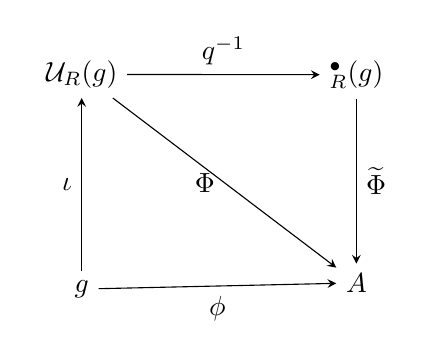
\begin{tikzpicture}
        \matrix (m)[
        matrix of math nodes,
        row sep=6em,
        column sep=7em
        ]
        {
          \mathcal{U}_R(\lie{g})
          & \Sym_R^{\bullet}(\lie{g}) \\
          \lie{g}
          & \algebra{A} \\
        };
        \draw
        [-stealth]
        (m-1-1) edge node [above] {$\lie{q}^{-1}$}
        (m-1-2) edge node [left] {$\Phi$}
        (m-2-2)
        (m-1-2) edge node [right] {$\widetilde{\Phi}$}
        (m-2-2)
        (m-2-1) edge node [left] {$\iota$}
        (m-1-1)
        (m-2-1) edge node [below] {$\phi$}
        (m-2-2);
    \end{tikzpicture}
\end{center}
where $\algebra{A}$ is an associative algebra as mentioned. Since we endowed 
$\algebra{U}_R(\lie{g}_z)$ and $\Sym_R^{\bullet}(\lie{g})$ with a topology, we 
can now ask if the homomorphisms $\Phi$ and $\widetilde{\Phi}$ are continuous. 
This question is partly answered by the following result:
\begin{proposition}[Universal property]
    \label{LCAna:Prop:Semi-functoriality}%
    Let $\lie{g}$ be an AE-Lie algebra, $\mathcal{A}$ an associative
    AE-algebra and $\phi \colon \lie{g} \longrightarrow \algebra{A}$
    is a continuous Lie algebra homomorphism.  If $R \geq 1$, then the
    induced algebra homomorphisms $\Phi$ and $\widetilde{\Phi}$ are
    continuous.
\end{proposition}
\begin{proof}
    We define an extension of $\Phi$ on the whole tensor algebra
    again:
    \begin{equation*}
        \Psi \colon
        \Tensor_R^{\bullet}(\lie{g})
        \longrightarrow
        \algebra{A},
        \quad
        \Psi
        =
        \widetilde{\Phi} \circ \Symmetrizer
    \end{equation*}
    It is clear that if $\Psi$ is continuous on factorizing tensors,
    we get the continuity of $\widetilde{\Phi}$ and of $\Phi$ via the
    infimum argument. So let $p$ be a continuous semi-norm on
    $\mathcal{A}$ with its asymptotic estimate $q$ and $\xi_1, \ldots,
    \xi_n \in \lie{g}$. Since $\phi$ is continuous, we find a
    continuous semi-norm $r$ on $\lie{g}$ such that for all $\xi \in
    \lie{g}$ we have $q(\phi(\xi)) \leq r(\xi)$. Then we have
    \begin{align*}
        p \left(
        \Psi \left(
        \xi_1 \tensor \cdots \tensor \xi_n
        \right) \right)
        & =
        p \left(
        \widetilde{\Phi} \left(
        \xi_1 \star_z \cdots \star_z \xi_n
        \right) \right)
        \\
        & =
        p( \phi(\xi_1) \cdots \phi(\xi_n) )
        \\
        & \leq
        q( \phi(\xi_1) )
        \cdots
        q( \phi(\xi_n) )
        \\
        & \leq
        r(\xi_1) \cdots r(\xi_n)
        \\
        & \leq
        r_R(\xi_1 \tensor \cdots \tensor \xi_n),
    \end{align*}
    where the last inequality is true for all $R \geq 0$ and hence for all 
    $R \geq 1$.
\end{proof}
Although this is a nice result, our construction fails to be
universal, since the universal enveloping algebra endowed with our
topology is \emph{not} AE in general. This is even very easy to see:
\begin{example}
    Take $\xi \in \lie{g}$, then we know that $\xi^{\tensor n} =
    \xi^{\ostar_z n} = \xi^n$ for $n \in \mathbb{N}$ where the formal
    parameter is $z = 1$. Let $R > 0$ and $p$ a continuous semi-norm
    in $\lie{g}$ then we find
    \begin{equation}
        p_R(\xi^n)
        =
        n!^R p(\xi)^n
        =
        \frac{n!^R}{c^n} q(\xi)^n
    \end{equation}
    for $c = \frac{p(\xi)}{q(\xi)}$ for a different semi-norm $q$ with
    $q(\xi) \neq 0$.  But since the $\frac{n!^R}{c^n}$ will always
    diverge for $n \rightarrow \infty$ we will never get an asymptotic
    estimate for $p_R$.
\end{example}
Although the construction is not universal, we can draw a nice conclusion 
from Proposition~\ref{LCAna:Prop:Semi-functoriality}:
\begin{corollary}[Continuous Representations]
    \label{LCAna:Coro:ContinuousRepresentations}%
    Let $R \geq 1$ and $\mathcal{U}_R(\lie{g})$ the universal
    enveloping algebra of an AE-Lie algebra $\lie{g}$, then for every
    continuous representation $\phi$ of $\lie{g}$ into the bounded
    linear operators $\Bounded(V)$ on a Banach space $V$ the induced
    homomorphism of associative algebras $\Phi \colon
    \mathcal{U}(\lie{g}) \longrightarrow \Bounded(V)$ is continuous.
\end{corollary}
\begin{proof}
    This follows directly from
    Proposition~\ref{LCAna:Prop:Semi-functoriality} and $\Bounded(V)$
    being a Banach algebra.
\end{proof}
\begin{remark}
	\mbox{}
	\begin{remarklist}
		\item
		From this, we get the special case that all finite-dimensional 
		representations of an AE-Lie algebra can be lifted to continuous 
		representations of $\algebra{U}(\lie{g}_z)$. We will come back to this 
		in the next section and see another result of it.
		
		\item
		For infinite-dimensional Lie algebras, this statement will not be very 
		important, since there, one rather has strongly continuous 
		representations and no norm-continuous ones. Nevertheless, our 
		topology may help to think about continuous linear functionals on 
		$\algebra{U}(\lie{g}_z)$ and to do finally some GNS-representation 
		theory of it. This would finally give us a representation of 
		$\algebra{U}(\lie{g}_z)$ on a (Pre-)Hilbert space and we could talk 
		about, what strongly continuous representations of the universal 
		enveloping algebra should be. In this sense, the results of this 
		chapter may also open a door towards some new approaches in this 
		field.
	\end{remarklist}
\end{remark}



\subsection{Functoriality}

Now let $\lie{g}, \lie{h}$ be two AE-Lie algebras. We know that a homomorphism 
of Lie algebras from $\lie{g}$ to $\algebra{U}(\lie{h}_z)$ would lift to a 
homomorphism $\algebra{U}(\lie{g}_z) \longrightarrow \algebra{U}(\lie{h}_z)$, 
if the latter one was AE, which is not the case. Yet, we would like to have 
this result and get the functoriality of our construction, but it won't be 
that easy. Let's draw the commutative diagram to make things clear:
\begin{center}
    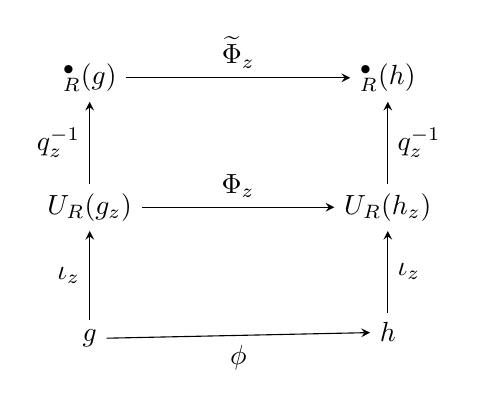
\begin{tikzpicture}
        \matrix (m)[
        matrix of math nodes,
        row sep=3em,
        column sep=7em
        ]
        {
          \Sym_R^{\bullet}(\lie{g})
          & \Sym_R^{\bullet}(\lie{h}) \\
          \algebra{U}_R(\lie{g}_z)
          & \algebra{U}_R(\lie{h}_z) \\
          \lie{g}
          & \lie{h} \\
        };
        \draw
        [-stealth]
        (m-1-1) edge node [above] {$\widetilde{\Phi}_z$}
        (m-1-2)
        (m-2-1) edge node [left] {$\mathfrak{q}_z^{-1}$}
        (m-1-1)
        (m-2-1) edge node [above] {$\Phi_z$}
        (m-2-2)
        (m-2-2) edge node [right] {$\mathfrak{q}_z^{-1}$}
        (m-1-2)
        (m-3-1)	edge node [below] {$\phi$}
        (m-3-2)
        (m-3-1)	edge node [left] {$\iota_z$}
        (m-2-1)
        (m-3-2)	edge node [right] {$\iota_z$}
        (m-2-2);
    \end{tikzpicture}
\end{center}
If $\phi$ is a continuous Lie algebra homomorphism, we want to know if 
$\Phi_z$ and $\widetilde{\Phi}_z$ will be continuous, too. Luckily, the answer 
is yes and our construction is functorial. For the proof, we will need the 
next lemma.
\begin{lemma}
    \label{LCAna:Lemma:LemmaPreContinuityN}%
    Let $\lie{g}$ be an AE-Lie algebra, $R \geq 1$ and $z \in
    \mathbb{C}$. Then for $p$ a continuous seminorm, $q$ an
    asymptotic estimate, $n \in \mathbb{N}$ and all $\xi_1, \ldots,
    \xi_n \in \lie{g}$ the following estimate
    \begin{equation}
        \label{LCAna:LemmaPreContinuityN}
        p_R \left(
            \xi_1 \star_z \cdots \star_z \xi_n
        \right)
        \leq
        c^n n!^R
        q^n(\xi_1 \tensor \cdots \tensor \xi_n)
    \end{equation}
    holds with $c = 8 \E (|z| + 1)$.
\end{lemma}
\begin{proof}
    We start with a continuous seminorm $p$:
    \begin{align}
        \nonumber
        p_R \left(
            \xi_1 \star_z \cdots \star_z \xi_n
        \right)
        & =
        p_R \Bigg(
        \sum\limits_{\ell = 0}^{n-1}
        \sum\limits_{\substack{
			1 \leq j \leq n-1 \\
			i_j \in \{0, \ldots, j\} \\
			\sum_{j = 1}^{n - 1} i_j = \ell
		}}
		z^{i_{n-1}}
		C_{i_{n-1}}
		\left(
			\ldots z^{i_2} C_{i_2}
			\left(
				z^{i_1} C_{i_1}
				\left( \xi_1, \xi_2 \right)
				, \xi_3
			\right)
			\ldots, \xi_n
		\right)
        \Bigg)
        \\
        \nonumber
        & \leq
        \sum\limits_{\ell = 0}^{n-1}
        (n - \ell)!^R
        \sum\limits_{\substack{
			1 \leq j \leq n-1 \\
			i_j \in \{0, \ldots, j\} \\
			\sum_{j = 1}^{n - 1} i_j = \ell
		}}
        p^{n - \ell} \Big(
		z^{i_{n-1}}
		C_{i_{n-1}}
		\left(
			\ldots z^{i_2} C_{i_2}
			\left(
				z^{i_1} C_{i_1}
				\left( \xi_1, \xi_2 \right)
				, \xi_3
			\right)
			\ldots, \xi_n
		\right)
		\Big)
        \\
        \nonumber
        & \leq
        \sum\limits_{\ell = 0}^{n-1}
        (n - \ell)!^R
        \sum\limits_{\substack{
			1 \leq j \leq n-1 \\
			i_j \in \{0, \ldots, j\} \\
			\sum_{j = 1}^{n - 1} i_j = \ell
		}}
        |B_{i_{n-1}}^*| \cdots |B_{i_1}^*|
        |z|^{i_{n-1}} \cdots |z|^{i_1}
        \\
        \label{LCAna:PreContinuityIntermediateN}
        & \quad \cdot
        \binom{1}{i_1} \binom{2 - i_1}{i_2}
        \cdots
        \binom{n - 1 - i_1 - \cdots i_{n-2}}{i_{n-1}}
        q(\xi_1) \cdots q(\xi_n)
    \end{align}
    By using the fact that $|B_m^*| \leq m!$ for all $m \in
    \mathbb{N}$ and grouping together the powers of $|z|$, we find
    \begin{align*}
        &p_R \left(
            \xi_1 \star_z \cdots \star_z \xi_n
        \right) \\
        &\quad\leq
        \sum\limits_{\ell = 0}^{n-1}
        (n - \ell)!^R
        \sum\limits_{\substack{
			1 \leq j \leq n-1 \\
			i_j \in \{0, \ldots, j\} \\
			\sum_{j = 1}^{n - 1} i_j = \ell
		}}
        |z|^{\ell}
        \frac{1!  (2 - i_1)! \cdots (n-1 - i_1 - \cdots - i_{n-2})!}
        {(1 - i_1)! \cdots (n-1 - i_1 - \cdots i_{n-1})!}
        q(\xi_1) \cdots q(\xi_n)
        \\
        &\quad\leq
        \sum\limits_{\ell = 0}^{n-1}
        (n - \ell)!^R
        \sum\limits_{\substack{
			1 \leq j \leq n-1 \\
			i_j \in \{0, \ldots, j\} \\
			\sum_{j = 1}^{n - 1} i_j = \ell
		}}
        |z|^{\ell}
        1^{i_1} 2^{i_2}
        \cdots (n-1)^{i_{n-1}}
        q(\xi_1) \cdots q(\xi_n)
        \\
        &\quad\leq
        \sum\limits_{\ell = 0}^{n-1}
        (n - \ell)!^R
        \sum\limits_{\substack{
			1 \leq j \leq n-1 \\
			i_j \in \{0, \ldots, j\} \\
			\sum_{j = 1}^{n - 1} i_j = \ell
		}}
        |z|^{\ell}
        n^{\ell}
        q(\xi_1) \cdots q(\xi_n)
        \\
        &\quad\leq
        \sum\limits_{\ell = 0}^{n-1}
        (n - \ell)!^R
        \sum\limits_{\substack{
			1 \leq j \leq n-1 \\
			i_j \in \{0, \ldots, j\} \\
			\sum_{j = 1}^{n - 1} i_j = \ell
		}}
        |z|^{\ell} (2 \E)^n \ell!
        q(\xi_1) \cdots q(\xi_n),
    \end{align*}
    where in the last step we used $n^{\ell} \leq \E^n
    \frac{n!}{(n-\ell)!} = \E^n \binom{n} {\ell} \ell! \leq \E^n 2^n
    \ell!$. But now we can simply estimate $|z|^{\ell} \leq (|z| +
    1)^n$ and $(n - \ell)!^R \ell! \leq n!^R$ for $R \geq 1$. We just
    need to count the number of summands and get
    \begin{align*}
        p_R \left(
            \xi_1 \star_z \cdots \star_z \xi_n
        \right)
        & \leq
        n!^R (2 \E)^n (|z| + 1)^n
        q(\xi_1) \cdots q(\xi_n)
        \sum\limits_{\ell = 0}^{n-1}
        \sum\limits_{\substack{
			1 \leq j \leq n-1 \\
			i_j \in \{0, \ldots, j\} \\
			\sum_{j = 1}^{n - 1} i_j = \ell
		}}
		1
        \\
        &\ot{(a)}{\leq}
        n!^R (2 \E)^n (|z| + 1)^n
        q(\xi_1) \cdots q(\xi_n)
        \sum\limits_{\ell = 0}^{n-1}
        \binom{n - 1 + \ell - 1}{\ell - 1}
        \\
        &\ot{(b)}{\leq}
        n!^R (2 \E)^n (|z| + 1)^n
        q(\xi_1) \cdots q(\xi_n)
        2^{2n}
        \\
        &\leq
        c^n n!^R q^n(\xi_1 \tensor \cdots \tensor \xi_n),
    \end{align*}
    with $c = 8 \E (|z| + 1)$. In ($a$) the estimate for the big sum
    is the following: for every $j = 1, \ldots, n-1$ we have surely
    $i_j \in \{0, 1, \ldots, n-1\}$ and the sum of all the $i_j$ is
    $\ell$. If we forget about all other restrictions, we will get
    even more terms. But then the number of summands is same as there
    are ways to distribute $\ell$ items on $n-1$ places, which is
    given by $\binom{n - 1 + \ell - 1}{\ell - 1}$. Then in ($b$) we
    use
    \begin{equation*}
        \binom{n - 1 + \ell - 1}{\ell - 1} \leq \binom{2 n}{\ell - 1}
    \end{equation*}
    with the binomial coefficient being zero for $\ell = 0$. Then it
    is just the standard estimate for binomial coefficients via the
    sum over all $\ell$.
\end{proof}
\begin{proposition}[Functoriality]
	\label{LCAna:Prop:Functoriality}
	Let $R \geq 1$, $\lie{g}, \lie{h}$ be AE-Lie algebras and $\phi \colon
	\lie{g} \longrightarrow \lie{h}$ a continuous homomorphism between them.
	Then it lifts to a continuous unital homomorphism of locally convex
	algebras $\Phi_z \colon \algebra{U}_R(\lie{g}_z) \longrightarrow
	\algebra{U}_R(\lie{h}_z)$.
\end{proposition}
\begin{proof}
	First, if $\phi \colon \lie{g} \longrightarrow \lie{h}$ is continuous, 
	then for every continuous seminorm $q$ on $\lie{h}$, we have a continuous 
	seminorm $r$ on $\lie{g}$ such that for all $\xi \in \lie{g}$
	\begin{equation*}
		q\left( \phi(\xi) \right)
		\leq
		r(\xi).
	\end{equation*}
	Second, we define $\Psi_z$ on factorizing tensors via
	\begin{equation*}
		\Psi_z \colon
		\Tensor_R^{\bullet}(\lie{g})
		\longrightarrow
		\Sym_R^{\bullet}(\lie{h})
		, \quad
		\Psi_z
		=
		\widetilde{\Phi}_z \circ
		\Symmetrizer
	\end{equation*}
	and extend it linearly to $\Tensor_R^{\bullet}(\lie{g})$. Clearly, 
	$\Phi_z$ and $\widetilde{\Phi}_z$ will be continuous if $\Psi_z$ is 
	continuous. From this, we get for a seminorm $p$ on $\lie{h}$, an 
	asymptotic estimate $q$ and $\xi_1, \ldots, \xi_n$
	\begin{align*}
		p_R\left(
			\Psi_z \left(
				\xi_1 \tensor \ldots \tensor \xi_n
			\right)
		\right)
		& =
		p_R \left(
			\phi \left( \xi_1 \right)
			\star_z \ldots \star_z
			\phi \left( \xi_1 \right)
		\right)
		\\
		& \ot{(a)}{\leq}
		c^n n!^R
		q \left( \phi \left( \xi_1 \right) \right)
		\ldots
		q \left( \phi \left( \xi_n \right) \right)
		\\
		& \ot{(b)}{\leq}
		c^n n!^R
		r \left( \xi_1 \right)
		\ldots
		r \left( \xi_n \right)
		\\
		& =
		(c r)_R\left( 
			\xi_1 \tensor \ldots \tensor \xi_n
		\right).
	\end{align*}
	Again, we use the infimum argument and we have the estimate on all tensor 
	in $\Tensor_R^{\bullet}(\lie{g})$. It extends to the completion and the 
	statement is proven.
\end{proof}



\section{Alternative topologies and an optimal result}
\label{sec:chap5_Optimality}

Let's set the formal parameter $z = 1$ for a moment and make some 
observations. So far, we found a topology on $\Sym_R^{\bullet}(\lie{g})$ which 
gives a continuous star product and which has a reasonably large completion, 
but it is always fair to ask if we can do better than that: we've seen that 
our completed algebra will not contain exponential series, which would be a 
very nice feature to have. So is it possible to put another locally convex 
topology on $\Sym_R^{\bullet}(\lie{g})$ which gives a completion with 
exponentials? The answer is no, at least under mild additional assumptions. 
\begin{proposition}[Optimality of the $R$-topology]
	\label{LCAna:Prop:NoBetterTopology}
	Let $\lie{g}$ be an AE Lie algebra in which one has elements $\xi, \eta$ 
	for which the Baker-Campbell-Hausdorff series does not converge. 
	Then there is no locally convex topology on $\Sym^{\bullet}(\lie{g})$ 
	such that all of the following things are fulfilled:
	\begin{propositionlist}
		\item
		The Gutt star product $\star_G$ is continuous.
		\item
		For every $\xi \in \lie{g}$ the series $\exp(\xi)$ converges 
		absolutely in the completion of $\Sym^{\bullet}(\lie{g})$.
		\item
		For all $n \in \mathbb{N}$ the projection and inclusion maps with 
		respect to the graded structure
		\begin{equation*}
			\Sym^{\bullet}(\lie{g})
	    		\ot{$\pi_n$}{\longrightarrow}
    	    		\Sym^n(\lie{g})
	    	    	\ot{$\iota_n$}{\longrightarrow}
	    		\Sym^{\bullet}(\lie{g})
		\end{equation*}
		are continuous.
	\end{propositionlist}
\end{proposition}
First of all, we should make clear what ''the Baker-Campbell-Hausdorff series 
does not converge'' actually means. This may be clear for a finite-dimensional 
Lie algebra, but in the locally convex setting, it is not that obvious. For 
simplicity, let's assume our local convex space to be complete in the 
following. First, we note here that a net or a sequence in a locally convex 
space is  convergent [or Cauchy], if it is convergent [or Cauchy] with respect 
to all $p \in \algebra{P}$. Quite similar to a normed space, we can make the 
following definition.
\begin{definition}
	\label{Def:RadiusOfConvergenceLCS}
	Let $V$ be a locally convex vector space, $\algebra{P}$ the set of 
	continuous semi-norms, $p \in \algebra{P}$ and 
	$\alpha = (\alpha_n)_{n \in \mathbb{N}}\subseteq V$ a sequence in $V$. 
	We set
	\begin{equation*}
		\rho_p(\alpha)
		=
		\left(
			\limsup_{n \longrightarrow \infty}
			\sqrt[n]{p \left(\alpha_n \right)}
		\right)^{-1}
	\end{equation*}
	where $\rho_p(\alpha) = \infty$ if $\limsup_{n \longrightarrow \infty} 
	\sqrt[n]{p \left(\alpha_n \right)} = 0$ as usual.
\end{definition}
From this, we immediately get the two following lemmas.
\begin{lemma}[Root test in locally convex spaces]
	\label{LCAna:Lemma:RootTest}
	Let $V$ be a complete locally convex vector space, $p \in \algebra{P}$ 
	and $\alpha = (\alpha_n)_{n \in \mathbb{N}} \subseteq V$ a sequence. 
	Then, if $\rho_p(\alpha) > 1$, the series
	\begin{equation*}
		\mathcal{S}_n(\alpha)
		=
		\sum\limits_{j = 0}^n
		\alpha_j
	\end{equation*}
	converges absolutely with respect to $p$. If, conversely, this
	series convegres with respect to $p$, then we have 
	$\rho_p(\alpha) \geq 1$.	
\end{lemma}
\begin{proof}
	The proof is completely analogous to the one in finite dimensions.
\end{proof}
\begin{lemma}
	\label{LCAna:Lemma:PowerSeriesConvAbs}
	Let $V$ be a complete locally convex vector space, $p \in \algebra{P}$, 
	$\alpha = (\alpha_n)_{n \in \mathbb{N}} \subseteq V$ a sequence and
	$M > 0$. Then, if the power series
	\begin{equation*}
		\lim_{n \longrightarrow \infty}
		\sum\limits_{j = 0}^n
		\alpha_j z^j
	\end{equation*}
	converges for all $z \in \mathbb{C}$ with $|z| \leq M$, it converges
	absolutely with respect to $p$ for all $z \in \mathbb{C}$ with $|z| < M$.
\end{lemma}
\begin{proof}
	Like in the finite-dimensional setting, we use the root test: Convergence 
	for $|z| \leq M$ means $\rho_p(\alpha_z) \geq 1$, where we have set 
	$\alpha_z = (\alpha_n z^n)_{n \in \mathbb{N}}$. Hence, for every $z' < z$ 
	we get $\rho_p(\alpha_{z'}) > 1$ and absolute convergence by Lemma 
	\ref{Lemma:LCAna:RootTest}.
\end{proof}
This helps us to make clear, what ''BCH does not converge'' can be 
interpreted. BCH can be read as a power series in two variables:
\begin{equation*}
	\bch{t \xi}{s \eta}
	=
	\sum\limits_{a,b = 0}^{\infty}
	t^a s^b
	\bchparts{a}{b}{\xi}{\eta}.
\end{equation*}
So if it converges for $\xi$ and $\eta$, then it converges absolutely for all 
$t \xi$ and $s \eta$ with $t,s \in [0, 1)$. If it converges for all $t \xi$ 
and $s \eta$ with $t, s \in \mathbb{K}$, then it converges absolutely for all 
$t, s$. If this is the case, we can reorder the sums as we like to, and the 
series
\begin{equation*}
	\sum\limits_{n = 0}^N
	\bchpart{n}{\xi}{\eta}
\end{equation*}
converges if and only if the series
\begin{equation*}
	\bch{t \xi}{s \eta}
	=
	\sum\limits_{a = 0}^{\infty}
	\sum\limits_{b = 0}^{\infty}
	\bchparts{a}{b}{\xi}{\eta}
\end{equation*}
converges. Now we can prove a Lemma, from which Proposition 
\ref{LCAna:Prop:NoBetterTopology} will follow immediately.
\begin{lemma}
	Let $\lie{g}$ be an AE Lie algebra and $\Sym^{\bullet}(\lie{g})$ is 
	endowed with a locally convex topology, such that the conditions $(i) - 
	(iii)$ from Proposition~\ref{Prop:LCAna:NoBetterTopology} are fulfilled. 
	Then the Baker-Campbell-Hausdorff series converges absolutely for all 
	$\xi, \eta \in \lie{g}$.
\end{lemma}
\begin{proof}
	First, we complete the algebra to $\widehat{\Sym}^{\bullet}(\lie{g})$.
	We will need the projection $\pi_1$ to the Lie algebra. Take 
	$\xi, \eta \in 	\lie{g}$. Now, since the the Gutt star product is 
	continuous and that the exponential series is absolutely convergent for 
	all $\xi, \eta \in \lie{g}$, we get for $t, s \in \mathbb{K}$
	\begin{align*}
		\pi_1 \left( \exp(t \xi) \star_G \exp(s \eta) \right)
		& =
		\pi_1
		\left(
			\lim_{N \rightarrow \infty}
			\left(
				\sum\limits_{n=0}^N
				\frac{t^n \xi^n}{n!}
			\right)
			\star_G
			\lim_{M \rightarrow \infty}
			\left(
				\sum\limits_{m=0}^M
				\frac{s^m \eta^m}{m!}
			\right)
		\right)
		\\
		& \ot{(a)}{=}
		\pi_1
		\left(
			\lim_{N \rightarrow \infty}
			\lim_{M \rightarrow \infty}
			\left(
				\sum\limits_{n=0}^N
				\frac{t^n \xi^n}{n!}
			\right)
			\star_G
			\left(
				\sum\limits_{m=0}^M
				\frac{s^m \eta^m}{m!}
			\right)
		\right)
		\\
		& \ot{(b)}{=}
		\lim_{N \rightarrow \infty}
		\lim_{M \rightarrow \infty}
		\pi_1
		\left(	
			\left(
				\sum\limits_{n=0}^N
				\frac{t^n \xi^n}{n!}
			\right)
			\star_G
			\left(
				\sum\limits_{m=0}^M
				\frac{s^m \eta^m}{m!}
			\right)
		\right)
		\\
		& \ot{(c)}{=}
		\lim_{N \rightarrow \infty}
		\lim_{M \rightarrow \infty}
		\sum\limits_{n,m=0}^{N, M}
		\bchparts{t \xi}{s \eta}{n}{m}
	\end{align*}
	where we used the continuity of the star product in (a), the continuity of 
	the projection in (b) and evaluated the projection in (c). Since 
	$\exp(t \xi)$ and $\exp(s \eta)$ are elements in the completion, their 
	star product exists and hence the double series at the end of this 
	equation converges for any two elements $\xi, \eta \in \lie{g}$. but now 
	we can use the result, that in this setting, the BCH series converges 
	absolutely. We can rearrange the terms and get the convergence of
	\begin{equation*}
		\sum\limits_{n = 1}^N
		\bchpart{n}{t \xi}{s \eta}.
	\end{equation*}
	Therefore, the BCH series must converge globally.
\end{proof}
Obviously, this proves Proposition~\ref{LCAna:Prop:NoBetterTopology}.


Now we want to use a result due to Wojty\'nski \cite{wojtynski:2000a}, who 
showed that for Banach-Lie algebras, global convergence of the BCH series is 
equivalent to the fact that for any $\xi$ we have
\begin{equation*}
	\norm{ 
		\left( \ad_{\xi} \right)^n 
	}^{\frac{1}{n}}
	\ot{$n \longrightarrow \infty$}{\longrightarrow}
	0.
\end{equation*}
A Banach-Lie algebra with this property is sometimes called quasi-nilpotent, 
radical or nil, see for example \cite{mueller:2000a} for various 
generalizations of nilpotency in the case of Banach algebras.
For finite-dimensional Lie algebras, quasi-nilpotency implies nilpotency. 
Hence for a finite-dimensional Lie algebra $\lie{g}$, BCH is globally 
convergent if and only if $\lie{g}$ is nilpotent.


From this, we see that at least for ''non-quasi-nilpotent'' Banach-Lie 
algebras, our result is in some sense optimal, at least if we want the grading 
structure to compatible with the topology.
\begin{remark}[Another topology in $\algebra{U}(\lie{g})$]
    \label{Rem:LCAnaBCHConvergence}
    In \cite{pflaum.schottenloher:1998a} Schottenloher and Pflaum mention an 
    alternative topology on the universal enveloping algebra for finite-
    dimensional Lie algebras: They took the coarsest locally convex topology, 
    such that all finite-dimensional representations of $\lie{g}$ extend to 
    continuous algebra homomorphisms. This topology is in fact even locally m-
    convex and has therefore an entire holomorphic calculus. In particular, 
    the completion will contain exponential functions for all Lie algebra 
    elements. Therefore, as we have seen in 
    Proposition~\ref{LCAna:Prop:NoBetterTopology}, it can not respect the 
    grading structure, as our topology does. The $R$-topology must hence be 
    different from that. As we have seen in 
    Proposition~\ref{Thm:LCAna:ContinuousRepresentations}, it is finer for 
    $R \geq 0$, ans since the topologies are different, it is strictly 
    finer.One could argue that the $R$-topology is ''just'' locally convex, 
    but its advantage (for our purpose) is that the grading is necessary for 
    the holomorphic dependence on the formal parameter, which is a wanted 
    feature.
\end{remark}





% Chapter 6
%


%
% Chapter 6 of my master thesis:
% The nilpotent case
%

\chapter{Nilpotent Lie algebras}

At the end of the last chapter, we have seen that the Baker-Campbell-Hausdorff 
series and its convergence plays an important role for a topology on the 
universal enveloping algebra. It is thus natural to ask whether things will 
change, if we look at Lie algebras from which have a globally convergent BCH 
series. To make things not too complicated from the beginning, we focus on 
locally convex and truly nilpotent Lie algebras. Recall that a Lie algebra 
$\lie{g}$ is nilpotent, if there exists a $N \in \mathbb{N}$, such that for 
all $n \geq N$ and all $\xi_1, \ldots, \xi_n \in \lie{g}$ we have
\begin{equation}
	\label{Nilpot:StrongNilpotency}
	\ad_{\xi_1} \circ \ldots \circ \ad_{\xi_n}
	=
	0.
\end{equation}
In the infinite-dimensional case, this is \emph{not} the same as 
\begin{equation*}
	\label{Nilpot:WeakNilpotency}
	\left( \ad_{\xi} \right)^n
	=
	0
\end{equation*}
for all $\xi \in \lie{g}$ and and $n \geq N$, but (typically strictly) 
stronger. In the case of finite-dimensional Lie algebras, the notions 
\eqref{Nilpot:StrongNilpotency} and \eqref{Nilpot:WeakNilpotency} coincide due 
to the so-called theorem of Engel, which makes use of the existence of a 
finite series of nilpotent ideals in the Lie algebra. Such a terminating 
series doesn't need to exist in infinite dimensions and there are known 
counter-examples to it.

Before we look at this case more closely, let's first make a list of things, 
that we expect to change or not when we go to this more particular setting.
\begin{enumerate}
	\item
	In Example~\ref{LCAna:Ex:HeisenbergAlgebra} we have seen that we can not 
	expect to get a continuous algebra structure for $R < 1$, even for very 
	simple nilpotent, but non-abelian Lie algebras. Therefore, we should not 
	expect to get much larger completions now.
	
	\item
	In \cite{waldmann:2014a}, Waldmann showed that the Weyl-Moyal star product 
	converges in the $R$-topology for $R \geq \frac{1}{2}$. This so-called 
	Weyl algebra is, however, nothing but a quotient of the Heisenberg 
	algebra. It would be interesting to understand this a bit better, since we 
	know that we need $R \geq 1$ for the latter. The quotient procedure must 
	therefore have some strong influence on this construction. Can we 
	reproduce the value $R \geq \frac{1}{2}$ somehow by dividing out an ideal?
	
	\item
	The argument we used in Propositipon~\ref{LCAna:Prop:NoBetterTopology},
	namely the non-global convergence of BCH, is not given any more. Now, we 
	don't have a reason any longer to expect that exponentials won't be part 
	of the completion. In this sense, it would be at least nice to have 
	something more than ''just'' $R = 1$. Can we do that?
	
	\item
	As already mentioned, there are generalizations or weaker forms of 
	nilpotency in infinite-dimensions, especially for Banach-Lie algebras, 
	which are equivalent to the usual notion of nilpotency in finite 
	dimensions. If we get a stronger result for nilpotent Lie algebras, can we 
	extend it to some of these generalizations?
\end{enumerate}
The very fascinating and highly interesting answer to the three questions we 
just posed is: yes, we can. The first section of this chapter will be devoted 
to the question from point $(iii)$: we get a bigger completion by using a 
projective limit. We will also see how to get again the nice functorial 
properties we had before. In second section, we will reproduce the result by 
Waldmann, at least for the finite-dimensional case. The third part will take 
care of some generalizations of nilpotentcy for Banach-Lie algebras and will 
extend the result of the projective limit to a particular subcase there.



 
\section{The projective limit} 
\label{sec:chap6_ProjLim} 

\subsection{Continuity of the Product}

As already mentioned, it is possible to extend the continuity result. 
Therefore, we take a locally convex, nilpotent Lie algebra $\lie{g}$ and look 
at
\begin{equation*}
	\Sym_{1^-}^{\bullet}(\lie{g})
	=
	\projlim_{\epsilon \longrightarrow 0}
	\Sym_{1 - \epsilon}^{\bullet}(\lie{g}).
\end{equation*}
A tensor is in the completion $\widehat{Sym}_{1^-}^{\bullet}(\lie{g})$, 
when it lies for every $\epsilon > 0$ in the completion or 
$\Sym_{1 - \epsilon}^{\bullet}(\lie{g})$. Otherwise stated: Let $\algebra{P}$ 
be the set of all continuous seminorms of the Lie algebra $\lie{g}$, then 
\begin{equation*}
	f \in \widehat{Sym}_{1^-}^{\bullet}(\lie{g})
	\quad \Longleftrightarrow \quad
	p_{1 - \epsilon} (x) 
	< 
	\infty
	\quad
	\forall_{p \in \algebra{P}}
	\forall_{\epsilon > 0}.
\end{equation*}
So, if we want to show, that the Gutt star product is continuous in 
$\widehat{Sym}_{1^-}^{\bullet}(\lie{g})$, we need to show that for every 
$p \in \algebra{P}$ and  $R < 1$, there exists a $q \in \algebra{P}$ and a 
$R' < 1$, such that for all $x,y \in \Sym^{\bullet}(\lie{g})$ we have
\begin{equation*}
	p_R \left(
		x \star_z y
	\right)
	\leq
	q_{R'}(x)
	q_{R'}(y).
\end{equation*}
Before we prove the next proposition, we want to remind that locally convex, 
nilpotent Lie algebras are always AE Lie algebras. So the results we have 
found so far, are valid in this case.
\begin{theorem}
    \label{Nilpot:Thm:ProjLimit}%
    Let $\lie{g}$ be a nilpotent locally convex Lie algebra with
    continuous Lie bracket and $N \in \mathbb{N}$ such that $N + 1$
    Lie brackets vanish.
    \begin{theoremlist}
	    	\item \label{item:Nilpot:CnOperators}
	    	If $0 \leq R < 1$, the $C_n$-operators are continuous and fulfil the 
	    	estimate
	    	\begin{equation}
	    		\label{eq:Nilpot:CnOperators}
	    		p_R \left(
	    			C_n (x, y)
	    		\right)
	    		\leq
	    		\frac{1}{2 \cdot 8^n}
	    		(32 \E q)_{R + \epsilon}(x)
	    		(32 \E q)_{R + \epsilon}(y),
	    	\end{equation}
	    	for all $x, y \in \Sym_R^{\bullet}(\lie{g})$, where $p$ is a 
	    	continuous seminorm, $q$ an asymptotic estimate and 
	    	$\epsilon = \frac{N - 1}{N}(1 - R)$.
	    	
	    	\item \label{item_Nilpot:SEinsMinus}
	    	The Gutt star product $\star_z$ is continuous for the locally convex 
	    	projective limit $\Sym_{1^-}^\bullet(\lie{g})$ and we have
	    	\begin{equation}
	    		\label{eq:Nilpot:Continuity}
	    		p_R \left(
	    			x \star_z y
	    		\right)
	    		\leq
	    		(c q)_{R + \epsilon}(x)
	    		(c q)_{R + \epsilon}(y)
	    	\end{equation}
	    	with $c = 32 \E (|z| +1)$ and the $\epsilon$ from the first part.
	    	The Gutt star product extends continuously to
	    	$\widehat{\Sym}_R^{\bullet}(\lie{g})$, where it converges absolutely 
	    	and coincides with the formal series.
    \end{theoremlist}
\end{theorem}
\begin{proof}
    Again we use $\star_z$ on the whole tensor algebra and compute the 
    estimate for $\xi^{\tensor k}$ and $\eta^{\tensor \ell}$. The important 
    point is that now, we get restrictions for the values of $n$.
    Recall that $k + \ell - n$ is the symmetric degree of $C_n \left( 
    \xi^{\tensor k}, \eta^{\tensor \ell} \right)$ and that we must have
    \begin{equation*}
	    	(k + \ell - n) N
    		\geq
    		k + \ell
    		\quad 
    		\Longleftrightarrow 
    		\quad
    		n 
    		\leq
    		(k + \ell)
    		\frac{N - 1}{N}
    \end{equation*}
    for $C_n \left( \xi^{\tensor k}, \eta^{\tensor \ell} \right) \neq 0$. 
    This makes it possible to estimate $n!^{1-R}$ in 
    \eqref{LCAna:CnOperators}: set $\delta = \frac{N - 1}{N}$ and also denote 
    a factorial where we have non-integers, meaning the gamma function. We get
    \begin{align*}
        n!^{1-R}
        & \leq
        (\delta (k + \ell)!)^{1 - R}
        \\
        & \leq
        (\delta (k + \ell))^{(1 - R) \delta (k + \ell)}
        \\
        & \leq
        (k + \ell)^{(1 - R) \delta (k + \ell)}
        \\
        & =
        \left(
            (k + \ell)^{(k + \ell)}
        \right)^{(1 - R) \delta}
        \\
        & \leq
        \left(
            \E^{k + \ell} 2^{k + \ell} k! \ell!
        \right)^{(1-R) \delta}
        \\
        & =
        \left( (2 \E)^{\delta (1-R)} \right)^{k + \ell}
        k!^{\epsilon} \ell!^{\epsilon},
    \end{align*}
    using $\epsilon = \delta (1 - R)$. Hence
    \begin{align*}
        p_R \left(
        	C_n \left(
        		\xi^{\tensor k}, \eta^{\tensor \ell}
        	\right)
        \right)
        & \leq
        \frac{
        	\left(
        		(2 \E)^{\delta (1 - R)}
        	\right)^{k + \ell}
        	k!^{\epsilon}
        	\ell!^{\epsilon}
        }{2 \cdot 8^n}
        (16 q)_R \left( \xi^{\tensor k} \right)
        (16 q)_R \left( \eta^{\tensor \ell} \right)
        \\
        & \leq
        \frac{1}{2 \cdot 8^n}
        (c q)_{R + \epsilon} \left( \xi^{\tensor k} \right)
        (c q)_{R + \epsilon} \left( \eta^{\tensor \ell} \right)
    \end{align*}
    with $c = 16 (2 \E)^{\delta (1 - R)} \leq 32 \E$.
    We then get the estimate on all tensors by the infimum argument and extend 
    it to the completion. Note, that for every $R < 1$ we also have 
    $R + \epsilon < 1$ with the $\epsilon = \delta(1-R)$ from above. Iterating 
    this continuity estimate, we get closer and closer to $1$ and it is not 
    possible to repeat this process an arbitrary number of times and stop at 
    some value strictly less than $1$. For the second part, we can conclude 
    analogously to the second part of 
    Proposition~\ref{LCAna:Prop:Continuity1}.
\end{proof}
Again, we can do an easier proof by assuming submultiplicativity of the 
seminorms, since we get an alternative version of 
Lemma~\ref{LCAna:Lemma:PreContinuity2}:
\begin{lemma}
	\label{Nilpot:Lemma:PreContinuity2}
	Let $\lie{g}$ be a locally m-convex, nilpotent Lie algebra such that more 
	$N$ nested Lie brackets vanish. Let $p$ be a continuous seminorm, 
	$z \in \mathbb{K}$ and $R \geq 0$. Then, for every tensor 
	$x \in \Sym_R^{\bullet}(\lie{g})$ of degree at most $k \in \mathbb{N}$ and 
	$\eta \in \lie{g}$, 	we have the estimate
	\begin{equation}
		\label{Nilpot:PreContinuity}
		p_R \left( x \star_z \eta \right)
		\leq
		(k + 1)^R k^{N (1-R)} c
		p_R (x) p(\eta)
	\end{equation}
	with the constant $c = \sum_{n = 0}^N \frac{|B_n^*|}{n!} |z|^n$.
\end{lemma}
\begin{proof}
	Again, we do the estimate on factorizing tensors and apply the infimum 
	argument later. So let $\xi, \eta \in \lie{g}$, $k \in \mathbb{N}$, $p$ a 
	continuous seminorm on $\lie{g}$ and $z \in \mathbb{K}$. Then, we have for 
	$R \geq 0$
	\begin{align*}
		p_R \left(
			\xi^{ \tensor k } \star_z \eta
		\right)
		& =
		\sum\limits_{n = 0}^k
		(k + 1 - n)!^R \binom{k}{n}
		|B_n^*| |z|^n
		p^{k + 1 - n} \left(
			\xi^{k-n}
			\left( \ad_{\xi} \right)^n (\eta)
		\right)
		\\
		& \leq
		(k + 1)^R
		\sum\limits_{n = 0}^N
		\frac{ k! (k-n)!^R }{ (k-n)! n! }
		|B_n^*| |z|^n
		p(\xi)^k p(\eta)
		\\
		& =
		(k + 1)^R
		p_R \left( \xi^{\tensor k} \right)
		p(\eta)
		\sum\limits_{n = 0}^N
		\left( \frac{k!}{(k-n)!} \right)^{1-R}
		\frac{|B_n^*| |z|^n}{n!}
		\\
		& \leq
		(k + 1)^R
		k^{N (1-R)}
		p_R \left( \xi^{\tensor k} \right)
		p(\eta)
		\sum\limits_{n = 0}^N
		\frac{|B_n^*| |z|^n}{n!}.
	\end{align*}
\end{proof}
Now, we can iterate Lemma~\ref{Nilpot:Lemma:PreContinuity2} in the same way, 
we did it in Chapter 5:
\begin{proof}[Alternative Proof of Theorem~\ref{Nilpot:Thm:ProjLimitConti}]
	Again, we do the calculation only on factorizing tensors. We need to 
	transform the $k^{N(1-R)}$ into a very small factorial somehow. This is 
	possible, since for given $N \in \mathbb{N}$ and $0 \leq R < 1$, the 
	sequence
	\begin{equation*}
		\left( \frac{k^N}{\sqrt{k!}} \right)^{1-R}
	\end{equation*}
	converges to $0$ for $k \longrightarrow \infty$ and is therefore bounded 
	by some $\kappa_N > 0$. Hence we get
	\begin{equation*}
		k^{ N (1-R) } 
		\leq
		\kappa_N \sqrt{k!}^{1-R},
	\end{equation*}
	and together with Lemma~\ref{Nilpot:Lemma:PreContinuity2} we find
	\begin{equation*}
		p_R \left( x \star_z \eta \right)
		\leq
		(k + 1)^R k!^{\frac{1-R}{2}} c \kappa_N
		p_R (x) p(\eta)
	\end{equation*}
	for any tensor $x$ of degree at most $k$. Now, we can iterate this result
	for $\xi, \eta \in \lie{g}$, $R \geq 0$, $k, \ell \in \mathbb{N}$:
	\begin{align*}
		p_R \left(
			\xi^{\tensor k} star_z \eta^{\tensor \ell}
		\right)
		& =
		p_R \left(
			\xi^{\tensor k} star_z 
			\eta^{\star_z \ell}
		\right)
		\\
		& \leq
		(k + \ell)^R
		(k + \ell - 1)!^{\frac{1-R}{2}}
		c \kappa_N
		p_R \left(
			\xi^{\tensor k} star_z 
			\eta^{\star_z (\ell - 1)}
		\right)
		p(\eta)
		\\
		& \leq
		\quad \vdots
		\\
		& \leq
		\left(
			\frac{(k + \ell)!}{k!}
		\right)^R
		(k + \ell - 1)!^{\frac{1-R}{2}}
		\ldots
		k!^{\frac{1-R}{2^N}}
		(c \kappa_N)^{\ell}
		p_R \left( \xi^{\tensor k} \right)
		p(\eta)^{\ell}
		\\
		& \leq
		\binom{k + \ell}{k}^R 
		\ell!^R
		(k + \ell)!^{\frac{(2^N - 1) (1-R)}{2^N} }
		(c \kappa_N)^{\ell}
		p_R \left( \xi^{\tensor k} \right)
		p(\eta)^{\ell}
		\\
		& \leq
		2^{(k + \ell) R}
		\ell!^R
		k!^{\frac{(2^N - 1) (1-R)}{2^N} }
		\ell!^{\frac{(2^N - 1) (1-R)}{2^N} }
		2^{ (k + \ell) \frac{(2^N - 1) (1-R)}{2^N} }
		(c \kappa_N)^{\ell}
		p_R \left( \xi^{\tensor k} \right)
		p(\eta)^{\ell}
		\\
		& \leq
		(2 p)_{R + \epsilon} 
		\left( \xi^{\tensor k} \right)
		(2 c \kappa_N p)_{R + \epsilon} 
		\left( \eta^{\tensor \ell} \right),
	\end{align*}
	where we have set $\epsilon = \frac{(2^N - 1)(1 - R)}{2^N}$. From this,
	we have clearly $R + \epsilon < 1$, and we get the wanted result for the 
	projective limit.
\end{proof}
Of course, the projective limit case gives us a bigger completion. We
immediately end up with the following result:
\begin{corollary}
    \label{corollary:NilpotentCase}%
    Let $\lie{g}$ be a nilpotent, locally convex Lie algebra.
    \begin{corollarylist}
    \item \label{item:NilpotentHasExp} 
    		Let $\exp(\xi)$ be the
        exponential series for $\xi \in \lie{g}$, the we have $\exp(t
        \xi) \in \widehat{\Sym}_{1^-}^\bullet(\lie{g})$ for all $t
        \in \mathbb{K}$.
    \item \label{item:NilpotentExpGivesBCH} 
    		For $\xi, \eta \in
        \lie{g}$ and $z \neq 0$ we have $\exp(\xi) \ostar_z
        \exp(\eta) = \exp \left(\frac 1 z \bch{z \xi}{z \eta}
        \right)$.
    \item \label{item:NipotentOneParameterGroups}
    		For $s,t \in
        \mathbb{K}$ and $\xi \in \lie{g}$ we have $\exp(t \xi)
        \ostar_z \exp(s \xi) = \exp ((t + s) \xi)$.
    \end{corollarylist}
\end{corollary}
\begin{proof}
    For the first part, recall that the completion of the projective
    limit $1^-$ will contain all those series $(a_n)_{n \in
      \mathbb{N}_0}$ such that
    \begin{equation*}
        \sum\limits_{n=0}^{\infty}
        a_n n!^{1 - \epsilon} c^n
        <
        \infty
    \end{equation*}
    for all $c > 0$.  This is the case for the exponential series of
    $t \xi$ for $t \in \mathbb{K}$ and $\xi \in \lie{g}$. The second
    part follows from the fact that all the projections $\pi_n$ onto
    the homogeneous subspaces $\Sym_{\pi}^n$ are continuous. The third
    part is then a direct consequence of the second.
\end{proof}


%
% A bit Functioriality also in this case
%

\subsection{Representations and Functoriality}
\label{subsec:NilpotentFunctorialityRepresentations}

In the general AE case, we had some useful results concerning representations 
of Lie algebras and the functorialty of our construction. These results can be 
extended to the projective limit $\Sym_{1^-}^{\bullet}(\lie{g})$.
\begin{proposition}[universal property]
	\label{Nilpot:Prop:UnivProperty}
	Let $\lie{g}$ be a locally convex nilpotent Lie algebra, $\algebra{A}$ an 
	associative AE algebra and $\phi \colon: \lie{g} \longrightarrow 
	\algebra{A}$ is a continuous homomorphism of Lie algebras. Then, the 
	lifted homomorphisms from $\Sym_{1^-}^{\bullet}(\lie{g})$ and 
	$\algebra{U}(\lie{g}_z)$ to $\algebra{A}$ are continuous.
\end{proposition}
\begin{proof}
	The proof is exactly the same as in the general AE case, since there, 
	$R \geq 0$ was enough.
\end{proof}
Again, this construction will be not a universal in the categorial sense, 
since $\Sym_{1^-}^{\bullet}(\lie{g})$ fails to be AE. But also here, we get 
the case of continuous representations into a Banach space (and in particular 
into a finite-dimensional space) as a corollary.
\begin{corollary}[Continuous Representations]
    \label{Nilpot:Coro:ContinuousRepresentations}%
    Let $\mathcal{U}_R(\lie{g})$ the universal enveloping algebra of locally 
    convex nilpotent Lie algebra $\lie{g}$, then for every continuous 
    representation $\phi$ of $\lie{g}$ into the bounded linear operators 
    $\Bounded(V)$ on a Banach space $V$, the induced homomorphism of 
    associative algebras $\Phi \colon \mathcal{U}(\lie{g}) \longrightarrow 
    \Bounded(V)$ is continuous.
\end{corollary}


We can also extend the functoriality statement to the projective limit, but we 
need to get another version of Lemma~\ref{Lemma:LCAna:LemmaPreContinuityN} for 
nilpotent Lie algebras, since thisis the corner stone of the functoriality 
proof.
\begin{lemma}
    \label{Lemma:Nilpot:LemmaPreContinuityN}%
    Let $\lie{g}$ be locally convex nilpotent Lie algebra and $N \in 
    \mathbb{N}$ such that $N + 1$ Lie brackets vanish, $0 \leq R < 1$ and 
    $z \in \mathbb{C}$. Then for $p$ a continuous seminorm, $q$ an
    asymptotic estimate, $n \in \mathbb{N}$ and all $\xi_1, \ldots,
    \xi_n \in \lie{g}$ the following estimate
    \begin{equation}
        \label{Nilpot:LemmaPreContinuityN}
        p_R \left(
            \xi_1 \star_z \cdots \star_z \xi_n
        \right)
        \leq
        c^n n!^{R + \epsilon}
        q^n(\xi_1 \tensor \cdots \tensor \xi_n)
    \end{equation}
    holds with $c = 16 \E^2 (|z| + 1)$ and $\epsilon = \frac{N-1}{N}(1 - R)$
    and the estimate is locally uniform in $z$.
\end{lemma}
\begin{proof}
    We take $R < 1$ and go directly into the proof of
    Lemma~\ref{Lemma:LCAna:LemmaPreContinuityN} at
    \eqref{LCAna:PreContinuityIntermediateN}.  We know that, since we
    may have at most $N$ brackets, also the values for $\ell$ are
    restricted to
    \begin{equation*}
        \ell
        \leq
        \frac{N-1}{N} n
        =
        \delta n
    \end{equation*}
    Using that in the proof of Lemma~\ref{Lemma:LCAna:LemmaPreContinuityN} 
    leads to
    \begin{align*}
        &p_R \left(
            \xi_1 \star_z \cdots \star_z \xi_n
        \right)
        \\
        &\quad\leq
        \sum\limits_{\ell = 0}^{\delta n}
        (n - \ell)!^R
        \sum\limits_{\substack{
			1 \leq j \leq n-1 \\
			i_j \in \{0, \ldots, j\} \\
			\sum_{j = 1}^{n - 1} i_j = \ell
		}}
        |z|^{\ell}
        \frac{1!  (2 - i_1)! \cdots (n-1 - i_1 - \cdots - i_{n-2})!}
        {(1 - i_1)! \cdots (n-1 - i_1 - \cdots - i_{n-1})!}
        q(\xi_1) \cdots q(\xi_n)
        \\
        &\quad\leq
        \sum\limits_{\ell = 0}^{\delta n}
        (n - \ell)!^R
        \sum\limits_{\substack{
			1 \leq j \leq n-1 \\
			i_j \in \{0, \ldots, j\} \\
			\sum_{j = 1}^{n - 1} i_j = \ell
		}}
        |z|^{\ell} (2 \E)^n \ell!
        q(\xi_1) \cdots q(\xi_n)
        \\
        &\quad\leq
        (2 \E)^n (|z| + 1)^n
        q(\xi_1) \cdots q(\xi_n)
        \sum\limits_{\ell = 0}^{\delta n}
        (n - \ell)!^R \ell!
        \binom{n + \ell - 2}{\ell - 1}
    \end{align*}
    We have
    \begin{equation*}
        \ell!
        =
        \ell!^R
        \ell!^{1-R}
        \leq
        \ell!^R
        \left(
            (\delta n)^{\delta n}
        \right)^{1-R}
        \leq
        \ell!^R
        n^{\delta n (1-R)}
        \leq
        \ell!^R
        n!^{\delta (1 - R)}
        \E^{\delta n (1 - R)}.
    \end{equation*}
    Together with $\ell!^R (n - \ell)!^R \leq n!^R$ this gives
    \begin{align*}
        p_R \left(
            \xi_1 \star_z \cdots \star_z \xi_n
        \right)
        & \leq
        (2 \E)^n (|z| + 1)^n
        n!^R n!^{\delta (1 - R)}
        q(\xi_1) \cdots q(\xi_n)
        \sum\limits_{\ell = 0}^{\delta n}
        \binom{n + \ell - 2}{\ell - 1}
        e^{\delta n (1 - R)}
        \\
        & \leq
        (2 \E)^n (|z| + 1)^n
        \left(\E^{(1-R) \delta}\right)^n
        4^n n!^{R + \epsilon}
        q(\xi_1) \cdots q(\xi_n),
    \end{align*}
    with $\epsilon = \delta (1-R)$. It is clear that for all $R < 1$ we have
    $R + \epsilon < 1$. Set 
    \begin{equation*}
    	c 
    	= 
    	8 \E (|z|+1) \E^{(1-R)\delta}
    	\leq
    	16 \E^2 (|z|+1)
	\end{equation*}
	and note that the estimate is locally uniform in $z$, even
    though it will not be uniform in $z$.
\end{proof}
\begin{proposition}
	\label{Nilpot:Prop:Functoriality}
	Let $R \geq 1$, $\lie{g}, \lie{h}$ be two locally convex nilpotent Lie 
	algebras and $\phi \colon \lie{g} \longrightarrow \lie{h}$ a continuous 
	homomorphism between them. Then it lifts to a continuous unital 
	homomorphism of locally convex algebras $\Phi_z \colon 
	\algebra{U}_R(\lie{g}_z) \longrightarrow \algebra{U}_R(\lie{h}_z)$.
\end{proposition}
\begin{proof}
	The proof is mostly analogous to the one of Proposition 
	\ref{LCAna:Prop:Functoriality}.
\end{proof}



\section{Module structures}
\label{sec:chap6_Modules}

The projective limit $1^-$ is not the only additional structure we will get, if 
our Lie algebra $\lie{g}$ is nilpotent. Lemma~\ref{Nilpot:Lemma:PreContinuity2} 
allows the existence of certain module structures, if the seminorms on 
$\lie{g}$ are in addition submultiplicative. For every $R \in \mathbb{R}$,the 
symmetric tensor algebra $\Sym_R^{\bullet}(\lie{g})$ is a locally convex vector 
space. For $R \geq 0$, the (symmetric) tensor product is continuous, which is 
very important for many estimates, and for $R \geq 1^-$, we have an algebra 
structure. In between however, we have more than ''only'' vector spaces: The 
spaces $\Sym_R^{\bullet}(\lie{g})$ form locally convex modules over the 
$\Sym_{R'}^{\bullet}(\lie{g})$ for certain values of $R'$. The next proposition 
will makes this more exact.
\begin{proposition}[Bimodules in $\Sym_R^{\bullet}(\lie{g})$]
	\label{Nilpot:Prop:Bimodules}
	Let $\lie{g}$ be a nilpotent, locally m-convex Lie algebra such that 
	$N + 1$ 	Lie brackets vanish, $z \in 	\mathbb{C}$ and $0 \leq R < 1$. 
	Then, for all $x, y \in \Sym^{\bullet}(\lie{g})$ and every continuous 
	seminorm $p$, we have the estimates
	\begin{align}
		\label{Nilpot:BimoduleEstimate1}
		p_R \left(
			x \star_z y
		\right)
		& \leq
		\left(2^{N + 1} p\right)_R(x) 
		\left(2^{N + 1} c p\right)_{R + N(1-R)}(y)
		\\
	\intertext{and}
		\label{Nilpot:BimoduleEstimate2}
		p_R \left(
			x \star_z y
		\right)
		& \leq
		\left(2^{N + 1} c p\right)_{R + N(1-R)}(x)
		\left(2^{N + 1} p\right)_R(y) 
	\end{align}
	with $c = \sum_{n = 0}^N \frac{|B_n^*| |z|^n}{n!}$.
	Hence, the vector space $\widehat{\Sym}_R^{\bullet}
	(\lie{g})$ forms a bimodule over the algebra $\widehat{\Sym}_{R + N(1-
	R)}^{\bullet}(\lie{g})$. In particular, if $\lie{g}$ is 2-step nilpotent, 
	the vector space $\widehat{\Sym}_0^{\bullet}(\lie{g})$ is a 
	$\widehat{\Sym}_1^{\bullet}(\lie{g})$-bimodule.
\end{proposition}
\begin{proof}
	Again, we do the calculation on factorizing tensors: Let 
	$\xi, \eta \in \lie{g}$, $R \geq 0$, $k, \ell \in \mathbb{N}$.
	Using Lemma~\ref{Nilpot:Lemma:PreContinuity2}, we get
	\begin{align*}
		p_R \left(
			\xi^{\tensor k} star_z \eta^{\tensor \ell}
		\right)
		& =
		p_R \left(
			\xi^{\tensor k} star_z 
			\eta^{\star_z \ell}
		\right)
		\\
		& \leq
		(k + \ell)^R
		(k + \ell - 1)^{N (1-R)}
		p_R \left(
			\xi^{\tensor k} star_z 
			\eta^{\star_z (\ell - 1)}
		\right)
		p(\eta)
		\\
		& \leq
		\quad \vdots
		\\
		& \leq
		\left(
			\frac{(k + \ell)!}{k!}
		\right)^R
		\left(
			\frac{(k + \ell - 1)!}{(k - 1)!}
		\right)^{N (1-R)}
		c^{\ell}
		p_R \left( \xi^{\tensor k} \right)
		p(\eta)^{\ell}
		\\
		& \leq
		2^{k + l} 2^{N (k + \ell)}
		\ell!^{N (1-R)}
		c^{\ell}
		p_R \left( \xi^{\tensor k} \right)
		p(\eta)^{\ell}
		\\
		& =
		\left(2^{N + 1} p\right)_R 
		\left( \xi^{\tensor k} \right)
		\left(2^{N + 1} c p\right)_{R + N(1-R)}
		\left( \eta^{\tensor \ell} \right).
	\end{align*}
	The proof of the second estimate is analogous.
\end{proof}
\begin{remark}[Possible extensions]
	This result immediately poses new questions, like the dependence on the 
	formal parameter in this case, possible generalizations to ''weaker forms'' 
	of nilpotency and so on. They may be issues of some future work, but can't
	be addressed here, since we rather want to present something like a part of 
	the ''big picture'' which is opened by the $R$-topology, instead of getting 
	lost in its details too much. There are, without any doubt, questions that 
	are more significant than extending those estimates to very special cases 
	and 	finding sharp bounds there, although this is interesting and important, 
	too.
\end{remark}
Although it seems clear from the construction, that these bimodules cannot be 
there for general Lie algebras, we can give a concrete counter-example, which 
shows that there are Lie algebras, which don't allow them.
\begin{example}
	\label{Nilpot:Ex:NoModulesInGeneral}
	Choose $R < 1$ and take $\lie{g} = \mathbbm{R}^3$ with the basis $e_1, e_2, 
	e_3$ and the vector product as Lie bracket:
	\begin{equation*}
		[e_1, e_2] 
		= 
		e_3 
		\qquad 
		[e_2, e_3] 
		= 
		e_1 
		\qquad 
		[e_3, e_1] 
		= 
		e_2
	\end{equation*}
	Again, we take a $\ell^1$-norm $n$ such that $n(e_1) = n(e_2) = n(e_3) 
	= 1$. It has the nice property that for $k, \ell, m \in \mathbb{N}$ we get
	on the projective tensor product
	\begin{equation*}
		n^{k + \ell + m} \left(
			e_1^k e_2^{\ell} e_3^m
		\right)
		=
		1.
	\end{equation*}
	Now we define the sequence $(a_k)_{k \in \mathbb{N}}$
	\begin{equation*}
		a_k 
		= 
		\frac{1}{k!^R} e_1^k,
	\end{equation*}
	for which we get $n_R(a_k) = 1$. Now, we want to show that 
	$a_k \star_z e_2$ grows faster than exponentially:
	\begin{align*}
		n_R \left( a_k \star_z e_2 \right) 
		& = 
		n_R \left( 
			\sum\limits_{j = 0}^k 
			\binom{k}{j} B_j^* 
			\frac{1}{k!^R} 
			e_1^{n-j} 
			\left( 
				\operatorname{ad}_{e_1} 
			\right)^j(e_2) 
		\right)
		\\
		& =
		\sum\limits_{j = 0}^k 
		\binom{k}{j} 
		|B_j^*| 
		\frac{1}{k!^R} 
		(k-j+1)!^R 
		\underbrace{
			n^{k-j} \left( e_1 (e_2 \wedge e_3) \right)
		}_{ = 1}
		\\
		& = 
		\sum\limits_{j = 0}^k 
		(k-j+1)^R 
		\binom{k}{j}
		\frac{|B_j^*|}{j!} 
		\frac{(k-j)!^R j^R}{k!^R} 
		j!^{1-R}
		\\
		& = 
		\sum\limits_{j=0}^k 
		(k-j+1)^R 
		\binom{k}{j}^{1-R} 
		\frac{|B_j^*|}{j!} 
		j!^{1-R}
		\\
		& \geq 
		\sum\limits_{j=0}^k 
		\frac{|B_j^*|}{j!} 
		j!^{1-R}
		\\
		& \geq 
		\frac{|B_k^*|}{k!^R}.
	\end{align*}
	We know, that for $R < 1$ and any $c > 0$
	\begin{equation*}
		\limsup_{n \longrightarrow \infty}
		\frac{|B_n^*|}{c^n n!^R}
		=
		\infty,
	\end{equation*}
	and hence the limes superior of $n_R \left( a_k \star_z e_2 \right) $ grows 
	faster than any exponential function.
\end{example}



\section{The Heisenberg and the Weyl algebra}
\label{sec:chap6_HeisenbergWeyl}

Now we want to see how we get the link to the Weyl algebra from
\cite{waldmann:2014a}, since we have something like a discrepancy for the
parameter $R$ concerning the continuity of the product in the Weyl and the 
Heisenberg algebra. In the following, we will show that this gap actually makes 
a lot of sense. For simplicity, we consider the easiest case of
the Weyl/Heisenberg algebra with two generators $Q$ and $P$, but the 
generalization to the Heisenberg [Weyl] algebra in $2n + 1$ [$2n$] dimensions 
is immediate and goes without problems. 
Recall that the Weyl algebra is a quotient of the enveloping algebra of the 
Heisenberg algebra $\lie{h}$ which one gets from dividing out its center. So 
let $\mathsf{h} \in \mathbb{C}$ and we have a projection
\begin{equation}
    \label{Nilpot:WeylProjection}
    \pi \colon
    \widehat{\Sym}_R^\bullet(\lie{h})
    \longrightarrow
    \widehat{\mathcal{W}}_R(\lie{h})
    =
     \left(
    	\frac{\Sym_R^\bullet(\lie{h})}
    	{\langle E - \mathsf{h} \Unit \rangle}
    \right)^{\widehat{} }
\end{equation}
Of course we want to know if this projection is continuous.
\begin{proposition}
    \label{proposition:ProjectionWeylContinuous}%
    The projection $\pi$ is continuous for $R \geq 0$.
\end{proposition}
\begin{proof}
    We extend $\pi$ to the whole tensor algebra by symmetrizing
    beforehand. Let then $p$ be a continuous seminorm on $\lie{h}$, $k,
    \ell, m \in \mathbb{N}_0$. We have
    \begin{align*}
        p_R(\pi (
        	Q^{\tensor k} \tensor
        	P^{\tensor \ell} \tensor
        	E^{\tensor m}
        ) )
        & =
        p_R( Q^k P^{\ell} \mathsf{h}^m )
        \\
        & =
        |\mathsf{h}|^m (k + \ell)!^R
        p^{k + \ell}(Q^k P^{\ell})
        \\
        & \leq
        (|\mathsf{h}| + 1)^{k + \ell + m}
        (k + \ell + m)!^R
        p(Q)^k p(P)^{\ell} p(E)^m
        \\
        & =
        ((|\mathsf{h}| + 1) p)_R
        (Q^{\tensor k} \tensor
        P^{\tensor \ell} \tensor
        E^{\tensor m}).
    \end{align*}
    Then we do the usual infimum argument and have the result on
    arbitrary tensors again.
\end{proof}


To establish the link to the continuity results of the Weyl algebra,
we need more: $\pi \circ \ostar_z$ should to be continuous for $R \geq \frac 
1 2$.
\begin{proposition}
    \label{proposition:ContinuousProductInWeyl}%
    Let $R \geq \frac{1}{2}$ and $\pi$ the projection from
    \eqref{Nilpot:WeylProjection}. Then the map $\pi \circ
    \ostar_z$ is continuous.
\end{proposition}
\begin{proof}
    We need to get the estimate on factorizing tensors: Let $p$ be a
    continuous seminorm, $q$ an asymptotic estimate and $k, k',
    \ell, \ell', m, m' \in \mathbb{N}_0$. Then we have to get an
    estimate for
    \begin{align*}
        p_R \left(
            \pi\left(
                Q^k P^{\ell} E^m \ostar_z Q^{k'} P^{\ell'} E^{m'}
            \right)
        \right).
    \end{align*}
    If we calculate the star product explicitly, we see, that we only
    get Lie brackets where we have $P$'s and $Q$'s. Let $r = k + \ell
    + m$ and $s = k' + \ell' + m'$, then we can actually simplify the
    calculations by
    \begin{align*}
        p_R \left(
        \pi(Q^k P^{\ell} E^m
        \ostar_z    Q^{k'} P^{\ell'} E^{m'}
        ) \right)
        & =
        (p_R \circ \pi) \left(
        \sum\limits_{n=0}^{r + s - 1}
        z^n C_n(Q^k P^{\ell} E^m,
        Q^{k'} P^{\ell'} E^{m'})
        \right)
        \\
        & \leq
        \sum\limits_{n=0}^{r + s - 1}
        |z|^n
        (p_R \circ \pi) \left(
        C_n(Q^k P^{\ell} E^m,
        Q^{k'} P^{\ell'} E^{m'})
        \right)
        \\
        & \leq
        \sum\limits_{n=0}^{r + s - 1}
        |z|^n
        (p_R \circ \pi) \left(
        C_n(Q^r, P^s)
        \right)
        \\
        & =
        \sum\limits_{n=0}^{r + s - 1}
        |z|^n
        \frac{r! s!}{(r-n)! (s-n)! n!}
        (p_R \circ \pi) \left(
        Q^{r-n} P^{s-n} E^n
        \right)
        \\
        & =
        \sum\limits_{n=0}^{r + s - 1}
        |z|^n |\mathsf{h}|^n
        \frac{r! s!}{(r-n)! (s-n)! n!}
        p_R \left(
        Q^{r-n} P^{s-n}
        \right)
        \\
        & \leq
        \sum\limits_{n=0}^{r + s - 1}
        |z|^n |\mathsf{h}|^n
        \frac{r! s!}{(r-n)! (s-n)! n!}
        \frac{(r + s - 2n)!^R}{r!^R s!^R}
        p_R \left(Q^{\tensor r} \right)
        p_R \left(P^{\tensor s} \right)
        \\
        & \leq
        \sum\limits_{n=0}^{r + s - 1}
        |z|^n |\mathsf{h}|^n
        \binom{r}{n} \binom{s}{n}
        \frac{(r + s - 2n)!^R n!}{r!^R s!^R}
        p_R \left(Q^{\tensor r} \right)
        p_R \left(P^{\tensor s} \right)
        \\
        & \leq
        \sum\limits_{n=0}^{r + s - 1}
        |z|^n |\mathsf{h}|^n
        \binom{r}{n} \binom{s}{n}
        \frac{(r + s - 2n)!^R n!}{r!^R s!^R}
        p_R \left(Q^{\tensor r} \right)
        p_R \left(P^{\tensor s} \right)
        \\
        & \ot{(a)}{\leq}
        \sum\limits_{n=0}^{r + s - 1}
        |z|^n |\mathsf{h}|^n
        \binom{r}{n} \binom{s}{n}
        \binom{r + s}{s}^R
        \binom{r + s}{2n}^{-R}
        p_R \left(Q^{\tensor r} \right)
        p_R \left(P^{\tensor s} \right)
        \\
        & \leq
        \sum\limits_{n=0}^{r + s - 1}
        (|z| + 1)^n (|\mathsf{h}| + 1)^n
        4^{r + s}
        p_R \left(Q^{\tensor r} \right)
        p_R \left(P^{\tensor s} \right)
        \\
        & \leq
        \underbrace{
        (8 (|z| + 1) (|c| + 1))^{r + s}
        }_{ = c^{r + s}}
        p_R \left(Q^{\tensor r} \right)
        p_R \left(P^{\tensor s} \right)
        \\
        & =
        (c p)_R \left(Q^{\tensor r} \right)
        (c p)_R \left(P^{\tensor s} \right)
        \\
        & \ot{(b)}{ = }
        (c p)_R \left(
        Q^{\tensor k} \tensor
        P^{\tensor \ell} \tensor
        E^{\tensor m} \right)
        (c p)_R \left(
        Q^{\tensor k'} \tensor
        P^{\tensor \ell'} \tensor
        E^{\tensor m'} \right),
    \end{align*}
    where in (a) we expanded the fraction with $(r + s)!^R$ to get the
    two binomial coefficients. It is clear, that this step just works
    for $R \geq \frac{1}{2}$.  In (b) we used the fact that we can ask
    for $p(Q) = p(P) = p(E)$. Now we just need to use
    \begin{equation*}
        \left(
        	Q^{\tensor k} \tensor
        	P^{\tensor \ell} \tensor
        	E^{\tensor m}
        \right)
        \ostar_z
        \left(
        	Q^{\tensor k'} \tensor
        	P^{\tensor \ell'} \tensor
        	E^{\tensor m'}
        \right)
        =
        Q^k P^{\ell} E^m
        \ostar_z
        Q^{k'} P^{\ell'} E^{m'}
    \end{equation*}
    in the first line and we are done, since we can use again the
    infimum argument to expand this estimate to all tensors.
\end{proof}
The previous proposition can be seen as something like the ''finite-dimensional 
version'' of Lemma 3.10 in \cite{waldmann:2014a}, just that we took a large 
detour for proving it. One could, most probably, redo some more results of this 
paper using finite-dimensional versions the Heisenberg algebra and the 
projection onto the Weyl algebra, but this would yield, also most probably, 
nothing new. It is good to know that this connections exists, but it is not 
something which is very helpful to pursue, since an evident generalization to 
infinite dimensions doesn't seem be quite easy.




\section{Banach-Lie algebras}
\label{sec:chap6_TheEProperty}

Now we want to focus a bit on weaker notions than true nilpotency. Since there 
are many of them, we want to focus on the easier case of Banach-Lie algebras, 
where a certain classification and quite a lot of results already exist.


\subsection{Generalizations of nilpotency}

In \cite{mueller:XXXXa}, M\"uller gives a list of weaker forms of nilpotency in 
associative Banach algebras. We can mostly copy the ideas and use it for 
Banach-Lie algebras, too
\begin{definition}
	Let $\lie{g}$ be a Banach-Lie algebra in which the Lie bracket fulfils the 
	estimate
	\begin{equation*}
		\norm{ [\xi, \eta] }
		\leq
		\norm{\xi}
		\norm{\eta}.
	\end{equation*}
	Denote by $\mathbb{B}_1(0)$ all elements $\xi \in \lie{g}$ with 
	$\norm{\xi} = 1$. We say that
	\begin{definitionlist}
		\item
		$\lie{g}$ is topologically nil (or radical, or quasi-nilpotent), if
		every $\xi \in \lie{g}$ is quasi-nilpotent, i.e.
		\begin{equation*}
			\lim_{n \longrightarrow \infty}
			\norm{\ad_{\xi}^n}^{\frac{1}{n}}
			=
			0.
		\end{equation*}
		
		\item
		$\lie{g}$ is uniformly topologically nil, if
		\begin{equation*}
			\lim_{n \longrightarrow \infty}
			\mathcal{N}_1(n)
			=
			0.
		\end{equation*}
		for
		\begin{equation}
			\mathcal{N}_1(n)
			=
			\sup \left\{ 
			\left.
				\norm{ \ad_{\xi}^n}^{\frac{1}{n}} 
			\right|
				\xi \in \mathbb{B}_1(0)
			\right\}.
		\end{equation}
		
		\item
		$\lie{g}$ is topologically nilpotent, if for every sequence
		$(\xi_n)_{n \in \mathbb{N}} \subset \mathbb{B}_1(0)$ we have
		\begin{equation*}
			\lim_{n \longrightarrow \infty}
			\norm{ 
				\ad_{\xi_1} \circ \ldots \circ \ad_{\xi_n}
			}^{\frac{1}{n}}
			=
			0.
		\end{equation*}
		
		\item
		$\lie{g}$ is uniformly topologically nilpotent, if
		\begin{equation*}
			\lim_{n \longrightarrow \infty}
			\mathcal{N}(n)
			=
			0.
		\end{equation*}
		for
		\begin{equation}
			\mathcal{N}(n)
			=
			\sup \left\{ 
			\left.
				\norm{ 
					\ad_{\xi_1} \circ \ldots \circ \ad_{\xi_n}
				}^{\frac{1}{n}} 
			\right|
				\xi_1, \ldots, \xi_n \in \mathbb{B}_1(0)
			\right\}.
		\end{equation}
	\end{definitionlist}
\end{definition}
It is clear that $(ii) \Rightarrow (i)$ and $(iv) \Rightarrow (iii)$. In the 
associative case, we have $(iii) \Leftrightarrow (iv)$ and hence $(iii) 
\Rightarrow (ii)$. Of course, it is a good question, if this remains true for 
Banach-Lie algebras. We have already encountered notion $(i)$: Wojty\'nski 
proved it to be equivalent to the fact that the BCH series converges globally 
in \cite{wojtynski:2000a}. In the following, we will make use of notion $(iv)$: 
we will show, that it is possible to generalize the result of Theorem 
\ref{Nilpot:Thm:ProjLimit} to this case.



\subsection{An adapted $R$-topology}

The idea will be to slightly change the topology: Instead of taking 
$n!^R$ as weights with $0 \leq R < 1$, we take sequence $(\alpha_n)_{n \in 
\mathbb{N}}$ (or just $(\alpha)$, for short) with a certain asymptotic 
behaviour for $n \longrightarrow \infty$ and use $\frac{n!}{\alpha_n}$ as 
weights. This will generalize the idea of $n!^R$ and be the starting point for 
the estimates.

First, we observe that every uniformly topologically nilpotent Banach-Lie 
algebra $\lie{g}$ comes with a characteristic, monotonously decreasing sequence
\begin{equation}
	\label{Nilpot:CharDownSequence}
	\omega_n
	=
	\sup_{m \geq n} \mathcal{N}(m).	
\end{equation}
If there exists a $N \in \mathbb{N}$, such that $\omega_n = 0$ for all $n \geq 
N$, then $\lie{g}$ is actually nilpotent and we can use the results of the 
first section in this chapter. We may hence restrict to those Banach-Lie 
algebras, where we have $\omega_n > 0$ for all $n \in \mathbb{N}$. This allows 
the next definition.
\begin{definition}[Rapidly increasing sequences]
	Let $\lie{g}$ be a uniformly topologically nilpotent Banach-Lie algebra and 
	$(\omega)$ the sequence defined in \eqref{Nilpot:CharDownSequence}. Then we 
	define the characteristic sequence $\chi(\lie{g})$ of $\lie{g}$ by
	\begin{equation}
		\label{Nilpot:CharSequence}
		\chi(\lie{g})_n
		=
		\max
		\left\{ 
			\frac{1}{\omega_n}
			,
			2
		\right\}.
	\end{equation}
	We moreover say, that a sequence $(\alpha)$ in $(1, \infty)$ is $\lie{g}$-
	rapidly increasing, if it fulfils the following properties:
	\begin{definitionlist}
		\item
		It grows fast than exponentially, i.e.
		\begin{equation*}
			\lim_{n \longrightarrow \infty}
			\frac{\log \left(\alpha_n \right)}{n}
			=
			\infty.
		\end{equation*}
		
		\item
		There exists a constant $c > 0$, such that
		\begin{equation*}
			\alpha_n 
			\leq 
			c^n  \chi(\lie{g})_n.
		\end{equation*}
	\end{definitionlist}
	We denote by $\algebra{I}_{\lie{g}}$ the set of all $\lie{g}$-rapidly 
	increasing sequences.
\end{definition}
Clearly, $(\chi(\lie{g}))$ is a $\lie{g}$-rapidly increasing series itself.
\begin{remark}
	The number $2$ in \eqref{Nilpot:CharSequence} may look a bit confusing at 
	the first sight, since it is somehow arbitrary, but for technical reasons, 
	we will need $\chi(g) > 1$ later. So actually every real number $c > 1$ 
	could have been put there. In this sense, the previous definition is rather 
	a technical tool than a ''general idea''.
\end{remark}
Each $(\alpha) \in \algebra{I}_{\lie{g}}$ gives a continuous seminorm 
$p_{\alpha}$ on the tensor algebra with the projective tensor product 
$\Tensor_{\pi}^{\bullet}(\lie{g})$ by
\begin{equation*}
	p_{\alpha}
	=
	\sum\limits_{n = 0}^{\infty}
	\frac{n!}{\alpha_n}
	\norm{\cdot}^{\tensor[\pi] n},
\end{equation*}
and we denote the set of all those seminorms by $\algebra{P}_{\lie{g}}$. 
Furthermore, For every sequence $(\xi_n)_{n \in \mathbb{N}} \subset 
\mathbb{B}_1(0)$ we get
\begin{equation*}
	\norm{
		[ \ldots [[\xi_1, \xi_2], \xi_3], \ldots \xi_n]
	}
	\leq
	\frac{2^n}{\chi(\lie{g})_n}.
\end{equation*}
Every rapidly increasing sequence $(\alpha)$ yields a continuous function 
$f_{\alpha}$ by
\begin{equation}
	\label{Nilpot:IncreasingFunction}
	f_{\alpha}
	\colon
	\mathbb{R}_0^+
	\longrightarrow
	\mathbb{R}^+
	, \quad
	f_{\alpha}(0)
	=
	2
	,\
	f_{\alpha}(n)
	=
	\log \left( \alpha_n \right)
	,\
	\forall_{n \in \mathbb{N}},
\end{equation}
and linear interpolation between the values at the integers. The idea behind is 
that this will allow us to use a lemma, which we now introduce. It is taken 
from a work \cite{mitiagin.rolewicz.zelazko:1962a} by Mitiagin, Rolewicz and 
\.{Z}elazko, where it is stated in Lemma~2.1 and Lemma~2.2.
\begin{lemma}
	\label{Nilpot:Lemma:MRZGrothLemma}
	Let $f\colon \mathbb{R}_0^+ \longrightarrow \mathbb{R}^+$ be a continuous 
	functions, such that
	\begin{equation}
		\label{Nilpot:GrowthProperty}
		\lim_{n \longrightarrow \infty}
		\frac{f(x)}{x}
		=
		\infty.
	\end{equation}
	Then there exists a convex, continuous function $g \colon \mathbb{R}_0^+ 
	\longrightarrow \mathbb{R}^+$, fulfilling \eqref{Nilpot:GrowthProperty} and
	\begin{equation}
		\label{Nilpot:SplittingProperty}
		g \left(
			t_1 + \ldots + t_n
		\right)
		\leq
		8 \left(
			g \left( t_1 \right)
			+ \ldots +
			g \left( t_n \right)
		\right)
		+
		f(n)
		, \quad
		\forall_{n \in \mathbb{N}}
		\text{ and all }
		t_i \in \mathbb{R}_0^+.
	\end{equation}
\end{lemma}
It is clear that Lemma~\ref{Nilpot:Lemma:MRZGrothLemma} is applicable to our 
function $f_{\alpha}$. 


\subsection{A new continuity result}

Now, we have finally prepared our toolbox well enough to prove a new result.
\begin{proposition}
	\label{Nilpot:Prop:TopNilBanachLie}
	Let $\lie{g}$ be a uniformly topologically nilpotent Banach-Lie algebra,
	$\alpha \in \algebra{I}_{\lie{g}}$, $p_{\alpha}$ the corresponding seminorm 
	according to \eqref{Nilpot:IncreasingFunction} and $z \in \mathbb{C}$. 
	Then, there exists a series $\beta = (\beta_n)_{n \in \mathbb{N}} \in 
	\algebra{I}_{\lie{g}}$, such that for all $x,y \in \Tensor_{\pi}^{\bullet}
	(\lie{g})$ we have the estimate
	\begin{equation}
		\label{Nilpot:TopNilBanachLie}
		p_{\alpha} \left(
			x \star_z y
		\right)
		\leq
		(c p)_{\beta} (x)
		(c p)_{\beta} (y)
	\end{equation}
	with a $c > 0$, which only depends on $\alpha$.
\end{proposition}
\begin{proof}
	We can again do the estimate on factorizing tensors and extend it with the 
	infimum argument later. Let hence $k, \ell \in \mathbb{N}$ and 
	$\xi, \eta \in \lie{g}$. we need to estimate the $C_n$-operators for $n = 
	0, 1, \ldots, k + \ell - 1$ and note therefore $r = k + \ell - n$ again.
	We get for $p_{\alpha} \in \algebra{P}_{\lie{g}}$
	\begin{align*}
		p_{\alpha} \left(
			C_n\left( \xi^{\tensor k}, \eta^{\tensor \ell} \right)
		\right)
		& =
		p_{\alpha}
		\bigg(
        		\frac{k! \ell!}{r!}
        		\sum\limits_{\substack{a_1, b_1, \ldots, a_r, b_r \geq 0 \\
            		a_i + b_i \geq 1 \\
            		a_1 + \ldots + a_r = k \\
            		b_1 + \ldots + b_r = \ell
          		}}
        		\bchparts{a_1}{b_1}{\xi}{\eta}
        		\ldots
        		\bchparts{a_r}{b_r}{\xi}{\eta}
        \bigg)
        \\
        & \leq 
    		\frac{k! \ell!}{r!}
    		\frac{r!}{\alpha_r}
    		\sum\limits_{\substack{a_1, b_1, \ldots, a_r, b_r \geq 0 \\
        		a_i + b_i \geq 1 \\
        		a_1 + \ldots + a_r = k \\
        		b_1 + \ldots + b_r = \ell
       	}}
       	\norm{
    			\bchparts{a_1}{b_1}{\xi}{\eta}
    		}
    		\ldots
    		\norm{
    			\bchparts{a_r}{b_r}{\xi}{\eta}
    		}
        \\
        & \leq
    		\frac{k! \ell!}{\alpha_r}
    		\sum\limits_{\substack{a_1, b_1, \ldots, a_r, b_r \geq 0 \\
        		a_i + b_i \geq 1 \\
        		a_1 + \ldots + a_r = k \\
        		b_1 + \ldots + b_r = \ell
       	}}
       	2^r 
       	\frac{1}{\chi(\lie{g})_{a_1 + b_1}}
       	\ldots
       	\frac{1}{\chi(\lie{g})_{a_r + b_r}}
       	\norm{\xi}^k
       	\norm{\eta}^{\ell},
    \end{align*}
	where we have used the estimate from Lemma 
	\ref{LCAna:Lemma:BCHTermsEstiamte} \textit{(\ref{Item:BCHEstimate})}
	in the last step. Rearranging this, we have
	\begin{equation*}
		p_{\alpha} \left(
			C_n\left( \xi^{\tensor k}, \eta^{\tensor \ell} \right)
		\right)
		\leq
    		k! \ell! 2^r
    		\norm{\xi}^k
       	\norm{\eta}^{\ell}
    		\sum\limits_{\substack{a_1, b_1, \ldots, a_r, b_r \geq 0 \\
        		a_i + b_i \geq 1 \\
        		a_1 + \ldots + a_r = k \\
        		b_1 + \ldots + b_r = \ell
       	}}
       	\frac{1}
       	{
       		\alpha_r
       		\cdot
       		\chi(\lie{g})_{a_1 + b_1}
       		\ldots
       		\chi(\lie{g})_{a_r + b_r}
       	},
	\end{equation*}
	and we would like to find a $(\beta) \in \algebra{I}_{\lie{g}}$ such that
	\begin{equation}
		\label{Nilpot:SavingSequence}
		\sup
		\left\{
		\left.
			\frac{\beta_k \cdot \beta_{\ell}}
	       	{
	       		\alpha_r
	       		\cdot
	       		\chi(\lie{g})_{a_1 + b_1}
	       		\ldots
	       		\chi(\lie{g})_{a_r + b_r}
	       	}
	    \right|
	    		k, \ell \in \mathbb{N},\
	    		a_i + b_i \geq 1,\
        		\sum_i a_i = k,\
        		\sum_j b_j = \ell
		\right\}
		\leq
		\kappa^{k + \ell}
	\end{equation}
	for some $\kappa > 0$, just depending on $(\alpha)$. Then we would have
	\begin{align*}
		p_{\alpha} \left(
			C_n\left( \xi^{\tensor k}, \eta^{\tensor \ell} \right)
		\right)
		& \leq
    		\frac{k! \ell!}{\beta_k \beta_{\ell}} 
    		2^r
    		\norm{\xi}^k
       	\norm{\eta}^{\ell}
    		\sum\limits_{\substack{a_1, b_1, \ldots, a_r, b_r \geq 0 \\
        		a_i + b_i \geq 1 \\
        		a_1 + \ldots + a_r = k \\
        		b_1 + \ldots + b_r = \ell
       	}}
       	\kappa^{k + \ell}
       	\\
       	& =
       	2^{-n}
       	(2 \kappa)^{k + \ell}
       	p_{\beta}
       	\left( \xi^{\tensor k} \right)
       	p_{\beta}
       	\left( \eta^{\tensor \ell} \right)
       	\sum\limits_{\substack{a_1, b_1, \ldots, a_r, b_r \geq 0 \\
        		a_i + b_i \geq 1 \\
        		a_1 + \ldots + a_r = k \\
        		b_1 + \ldots + b_r = \ell
       	}}
       	1
       	\\
       	& \leq
       	\frac{1}{2 \cdot 8^n} 
       	(16 \kappa)^{k + \ell}
       	p_{\beta}
       	\left( \xi^{\tensor k} \right)
       	p_{\beta}
       	\left( \eta^{\tensor \ell} \right)
       	\\ 
       	& =
       	\frac{1}{2 \cdot 8^n} 
       	(16 \kappa p)_{\beta}
       	\left( \xi^{\tensor k} \right)
       	(16 \kappa p)_{\beta}
       	\left( \eta^{\tensor \ell} \right).
    \end{align*}
    From this we could conclude analogously to the procedure in the proof of 
    Theorem~\ref{Thm:LCAna:Continuity1} and the statement would be proven.
    We now need to show the existence of a $(\beta) \in \algebra{I}_{\lie{g}}$ 
    and a $\kappa > 0$, such that \eqref{Nilpot:SavingSequence} holds.
    \begin{claim}
    		For $f_{\alpha}$ defined as in \eqref{Nilpot:IncreasingFunction}, we 
    		take the function $g$ we get from 
    		Lemma~\ref{Nilpot:Lemma:MRZGrothLemma}. Then the sequence $(\beta)$ 
    		defined by
    		\begin{equation}
    			\beta_n
    			=
    			\exp \left(
    				\frac{g(n)}{8}
    			\right)
    		\end{equation}
    		and $\kappa = c' \E^{8 g(1)}$ have the desired properties, where 
    		$c' > 0$ is a constant, such that $\alpha_n \leq c'^n \chi(\lie{g})_n$.
    \end{claim}
    \begin{subproof}
    		First note that there is a fixed $c' > 0$
    		\begin{equation*}
    			\frac{1}{\chi(\lie{g})_n}
    			\leq
    			\frac{c'^n}{\alpha_n}
    		\end{equation*}
    		Denote $a_i + b_i = n_i$. Then we have
    		\begin{equation*}
    			\frac{\beta_k \cdot \beta_{\ell}}
	       	{
	       		\alpha_r
	       		\cdot
	       		\chi(\lie{g})_{n_1}
	       		\ldots
	       		\chi(\lie{g})_{n_r}
	       	}
	       	\leq
    			\frac{c'^{k + \ell} \beta_k \cdot \beta_{\ell}}
	       	{
	       		\alpha_r
	       		\cdot
	       		\alpha_{n_1}
	       		\ldots
	       		\alpha_{n_r}
	       	}
    		\end{equation*}
    		and hence
    		\begin{align*}
    			\log \left(
    				\frac{\beta_k \cdot \beta_{\ell}}
		       	{
		       		\alpha_r
		       		\cdot
		       		\chi(\lie{g})_{a_1 + b_1}
		       		\ldots
		       		\chi(\lie{g})_{a_r + b_r}
		       	}
	       	\right)
	       	& \leq
    			\log \left(
    				\frac{c'^{k + \ell} \beta_k \cdot \beta_{\ell}}
		       	{
		       		\alpha_r
		       		\cdot
		       		\alpha_{n_1}
		       		\ldots
		       		\alpha_{n_r}
		       	}
	       	\right)
	       	\\
	       	& =
	       	(k + \ell) \log(c')
	       	+
	       	\frac{g(k)}{8}
	       	+
	       	\frac{g(\ell)}{8}
	       	-
	       	f_{\alpha}(r)
	       	-
	       	f_{\alpha}(n_1)
	       	- \ldots -
	       	f_{\alpha}(n_r)
	       	\\
	       	& \ot{(a)}{\leq}
	       	(k + \ell) \log(c')
	       	+
	       	\frac{g(k + \ell)}{8}
			-
	       	f_{\alpha}(r)
	       	-
	       	f_{\alpha}(n_1)
	       	- \ldots -
	       	f_{\alpha}(n_r)
	       	\\
	       	& \ot{(b)}{\leq}
			(k + \ell) \log(c')
	       	+
	       	g(n_1) + \ldots + g(n_r)
	       	+
	       	\frac{f_{\alpha}(r)}{8}
	       	\\
	       	& \qquad
	       	-
	       	f_{\alpha}(r)
	       	-
	       	f_{\alpha}(n_1)
	       	- \ldots -
	       	f_{\alpha}(n_r)
	       	\\
	       	& \ot{(c)}{\leq}
	       	(k + \ell) \log(c')
	       	+
	       	\left( g(n_1) - f_{\alpha}(n_1) \right)
	       	+ \ldots + 
	       	\left( g(n_r) - f_{\alpha}(n_r) \right)
	       	\\
	       	& \ot{(d)}{\leq}
	       	(k + \ell) \log(c')
	       	+
	       	8 g(1) n_1
	       	+ \ldots + 
	       	8 g(1) n_r
	       	\\
	       	& =
	       	(k + \ell)
	       	(\log(c') + 8 g(1)),
    		\end{align*}
    		where we have used the convexity of $g$ in (a), 
    		Lemma~\ref{Nilpot:Lemma:MRZGrothLemma} in (b) and $\frac{g(n)}{8} \leq 
    		g(n)$ in (c). In (d) we used the lemma again by estimating
    		\begin{equation*}
    			g(n)
    			=
    			g(1 + \ldots - 1)
    			\leq
    			8 n g(1) + f_{\alpha}(n).
    		\end{equation*}
    		This shows that $\kappa = c' \E^{8 g(1)}$ really gives the estimate.
    \end{subproof}
    Now, we only need to sum up the $|z|^n C_n\left( \xi^{\tensor} k, 
    \eta^{\tensor \ell} \right)$. We know this is possible from Chapter 5, and 
    we finally get a continuity estimate which is locally uniform in $z$.
\end{proof}


At the end of Chapter 5, we showed that a finite-dimensional Lie algebra 
$\lie{g}$ is nilpotent if and only if its universal enveloping algebra 
$\algebra{U}(\lie{g})$ admitted a locally convex topology, such that the 
following three things are fulfilled:
\begin{enumerate}
	\item
	The product in $\algebra{U}(\lie{g})$ is continuous.

	\item
	For every $\xi \in \lie{g}$ the series $\exp(\xi)$ converges 
	absolutely in the completion of $\algebra{U}(\lie{g})$.

	\item
	Pulling back the topology to the symmetric tensor algebra, the projection 
	and inclusion maps with respect to the graded structure
	\begin{equation*}
		\Sym^{\bullet}(\lie{g})
    		\ot{$\pi_n$}{\longrightarrow}
   	    		\Sym^n(\lie{g})
    	    	\ot{$\iota_n$}{\longrightarrow}
    		\Sym^{\bullet}(\lie{g})
	\end{equation*}
	are continuous for all $n \in \mathbb{N}$.
\end{enumerate}
For Banach-Lie algebras, we came quite close to a similar statement: We know 
from Proposition~\ref{LCAna:Prop:NoBetterTopology} and the result of 
Wojty\`nski, that a Banach-Lie algebra must at least be \emph{topologically 
nil} to satisfy the three upper points. We also know, that a uniformly 
topologically nilpotent Banach-Lie algebra $\lie{g}$ allows us to construct 
such a locally convex topology on $\algebra{U}(\lie{g})$ explicitly. Maybe it 
is possible to find a notion of generalized nilpotency, which characterizes 
those three points exactly.





% Chapter 7
%


%
% Chapter 7 of my master thesis:
% The Hopf algebra structure
%

\chapter{The Hopf Algebra Structure}

As already pointed out in Chapter 3, universal enveloping algebras of a Lie 
algebras are more than just associative, unital algebras: they constitute one of 
the most important types of \emph{Hopf algebras}, which are very common 
structures in mathematics. Hopf algebras are a particular \emph{bialgebras}, 
which in turn are on one hand associative, unital algebras, and on the other hand 
coassociative, counital coalgebras. Those two substructures of bialgebras must of 
course fulfil certain compatibility conditions. Note at this point, that 
coalgebras play a crucial role in the theory of formal deformation quantization, 
which is due to Kontsevich, but which has been a lot further developed since. 
Good references on this so-called formality theory are given by Esposito 
\cite{esposito:2015a}.

In a Hopf algebra however, we have an 
additional map, called the \emph{antipode}, which again must fulfil some 
compatibility relations. So, in brief, a Hopf algebra over a field $\mathbb{K}$ 
is a tuple $(H, \cdot, \eta, \Delta, \varepsilon, S)$ of a vector space $H$ 
together with the following maps
\begin{equation*}
\begin{array}{rlrl}
	\cdot \colon
	&
	H \tensor H 
	\longrightarrow
	H, 
	& \quad &
	\text{ multiplication}
	\\
	\eta \colon
	&
	\mathbb{K}
	\longrightarrow
	H
	, 
	& \quad &
	\text{ unit}
	\\
	\Delta \colon
	&
	H
	\longrightarrow
	H \tensor H
	, & \quad &
	\text{ coproduct}
	\\
	\varepsilon \colon
	&
	H
	\longrightarrow
	\mathbb{K}
	, & \quad &
	\text{ counit}
	\\
	S \colon
	&
	H
	\longrightarrow
	H
	, & \quad &
	\text{ antipode},
\end{array}
\end{equation*}
such that we have a certain set of commuting diagrams. A very nice introduction 
to the theory of Hopf algebras with a lot of examples can e.g. be found in 
\cite{schweigert:2015a:script}.


In the previous chapters, we have mostly studied the properties of the 
multiplication in $\algebra{U}(\lie{g}_z)$, endowed with a particular topology. 
In this last chapter of this thesis, we will treat the remaining Hopf algebra 
structure maps. In the first section, we will see that the comultiplication and 
the antipode are not touched by our deformation procedure. Hence, it will be 
enough to show the continuity of the undeformed versions of those maps, which we 
will do in second section.



\section{An Undeformed Hopf Structure}

To get show the continuity of the remaining structure maps of 
$\algebra{U}_R(\lie{g}_z)$, we have to put estimates on seminorms again. For this 
purpose, we need explicit formulas for the antipode
\begin{equation}
    \label{eq:Antipode}
    S_z \colon
    \algebra{U}(\lie{g}_z)
    \longrightarrow
    \algebra{U}(\lie{g}_z)
\end{equation}
and the coproduct
\begin{equation}
    \label{eq:CoProduct}
    \coproduct_z \colon
    \algebra{U}(\lie{g}_z)
    \longrightarrow
    \algebra{U}(\lie{g}_z)
    \tensor
    \algebra{U}(\lie{g}_z)
\end{equation}
in the $\algebra{U}_R(\lie{g}_z)$ and in $\Sym^{\bullet}(\lie{g})$. We pull them 
back to the symmetric algebra and extend them to the whole tensor algebra by 
symmetrizing beforehand. We define
\begin{equation}
    \label{eq:AntipodeOnTensor}
    \widetilde{S}_z \colon
    \Tensor^\bullet(\lie{g})
    \longrightarrow
    \Sym^\bullet(\lie{g})
    , \quad
    \widetilde{S}_z
    =
    \mathfrak{q}_z^{-1}
    \circ
    S_z
    \circ
    \mathfrak{q}_z
    \circ
    \Symmetrizer
\end{equation}
and
\begin{equation}
    \label{eq:CoProductOnTensor}
    \widetilde{\ocoproduct}_z \colon
    \Tensor^\bullet(\lie{g})
    \longrightarrow
    \Sym^\bullet(\lie{g})
    \tensor
    \Sym^\bullet(\lie{g})
    , \quad
    \widetilde{\ocoproduct}_z
    =
    (\mathfrak{q}_z^{-1} \tensor \mathfrak{q}_z^{-1})
    \circ
    \coproduct_z
    \circ
    \mathfrak{q}_z
    \circ
    \Symmetrizer,
\end{equation}
to avoid that the maps on $\Sym^{\bullet}(\lie{g})$ and on $\algebra{U}
(\lie{g}_z)$ are denoted by the same symbols. The next lemma gives us the two 
explicit formulas we need.
\begin{lemma}
    \label{Thm:Hopf:Formulas}%
    For $\xi_1, \ldots, \xi_n \in \lie{g}$ we have the identities
    \begin{equation}
        \label{Hopf:AntipodeFormula}
        \widetilde{S}_z
        \left( \xi_1 \tensor \cdots \tensor \xi_n \right)
        =
        (-1)^n
        \xi_1 \cdots \xi_n
    \end{equation}
    and
    \begin{equation}
        \label{Hopf:CoproductFormula}
        \widetilde{\ocoproduct}_z
        \left(\xi_1 \tensor \cdots \tensor \xi_n \right)
        =
        \sum\limits_{
        	I \subseteq
        	\{1, \ldots, n\}
        }
        \xi_I
        \tensor
        \xi_1 \cdots
        \widehat{\xi_I}
        \cdots \xi_n
    \end{equation}
    where $\xi_I$ denotes the symmetric tensor product of all $\xi_i$ with 
    $i \in I$ and $\widehat{\xi_I}$ means that the $\xi_i$ with $i \in I$ 
    are left out.
\end{lemma}
\begin{proof}
	First, we derive Formula \ref{Hopf:AntipodeFormula}: the antipode gives
	$S_z(\xi) = - \xi$ for $\xi \in \lie{g}$ and extends to $\algebra{U}
	(\lie{g}_z)$ by algebra antihomomorphism, hence
	\begin{equation*}
		S_z \left( 
			\xi_1 \odot \cdots \odot \xi_n
		\right)
		=
		(-1)^n
		\xi_n \odot \cdots \odot \xi_1
	\end{equation*}
	in $\algebra{U}(\lie{g}_z)$ for $\xi_1, \ldots, \xi_n \in \lie{g}$.
	This means
	\begin{equation*}
		\widetilde{S}_z \left( 
			\xi_1 \star_z \cdots \star_z \xi_n
		\right)
		=
		(-1)^n
		\xi_n \star_z \cdots \star_z \xi_1
	\end{equation*}	
	in $\Sym^{\bullet}(\lie{g})$. But now, using the linearity of 
	$\widetilde{S}_z$ we get
	\begin{align*}
		\widetilde{S}_z \left( \xi_1 \cdots \xi_n \right)
		& =
		\widetilde{S}_z \left( 
		\frac{1}{n!}
			\sum\limits_{\sigma \in S_n}
			\xi_{\sigma(1)} 
			\star_z \cdots \star_z 
			\xi_{\sigma(n)}
		\right)
		\\
		& =
		\frac{1}{n!}
		\sum\limits_{\sigma \in S_n}
		\widetilde{S}_z \left( 
			\xi_{\sigma(1)} 
			\star_z \cdots \star_z 
			\xi_{\sigma(n)}
		\right)
		\\
		& =
		\frac{1}{n!}
		\sum\limits_{\sigma \in S_n}
		(-1)^n
		\xi_{\sigma(n)} 
		\star_z \cdots \star_z 
		\xi_{\sigma(1)}
		\\
		& =
		(-1)^n
		\xi_1 \cdots \xi_n.
	\end{align*}
	For the coproduct, we have well-known formula with shuffle permutations:
	\begin{equation*}
		\ocoproduct_z \left(
			\xi_1 \odot \cdots \odot \xi_n
		\right)
		=
		\sum\limits_{k=0}^n
		\sum\limits_{\substack{
			1 \leq i_1
			< \ldots <
			i_k \leq n
			\\
			I = \{i_1, \ldots, i_k\}
		}}
		\xi_{i_1} \odot \cdots \odot \xi_{i_k}
		\tensor
		\xi_1 
		\odot \cdots 
		\widehat{\xi_I}
		\cdots \odot
		\xi_n.
	\end{equation*}
	We can derive it from the fact that $\ocoproduct_z$ has the following form on 
	Lie algebra elements:
	\begin{equation*}
		\ocoproduct_z (\xi)
		=
		\xi \tensor \Unit
		+
		\Unit \tensor \xi.
	\end{equation*}
	The coproduct extends to $\algebra{U}(\lie{g}_z)$ by algebra 
	homomorphism. This yields
	\begin{align*}
		\ocoproduct_z \left(
			\xi_1 \odot \cdots \odot \xi_n
		\right)
		& =
		\ocoproduct_z \left( \xi_1 \right)
		\odot \cdots \odot
		\ocoproduct_z \left( \xi_n \right)
		\\
		&=
		\left( \xi_1 \tensor \Unit + \Unit \tensor \xi_1 \right)
		\odot \cdots \odot
		\left( \xi_n \tensor \Unit + \Unit \tensor \xi_n \right)
		\\
		&=
		\sum\limits_{k=0}^n
		\sum\limits_{\substack{
			1 \leq i_1
			< \ldots <
			i_k \leq n
			\\
			I = \{i_1, \ldots, i_k\}
		}}
		\xi_{i_1} \odot \cdots \odot \xi_{i_k}
		\tensor
		\xi_1 
		\odot \cdots 
		\widehat{\xi_I}
		\cdots \odot
		\xi_n.
	\end{align*}
	Now we can pull this back to $\Sym^{\bullet}(\lie{g}_z)$. We get a $\star_z$ 
	for every $\odot$. For symmetric tensors we have by linearity
	\begin{align*}
		&
		\widetilde{\ocoproduct}_z 
		\left( \xi_1 \cdots \xi_n \right)
		\\
		& =
		\widetilde{\ocoproduct}_z \left( 
			\frac{1}{n!}
			\sum\limits_{\sigma \in S_n}
			\xi_{\sigma(1)} 
			\star_z \cdots \star_z 
			\xi_{\sigma(n)}
		\right)
		\\
		& =
		\frac{1}{n!}
		\sum\limits_{\sigma \in S_n}
		\widetilde{\ocoproduct}_z \left( 
			\xi_{\sigma(1)} 
			\star_z \cdots \star_z 
			\xi_{\sigma(n)}
		\right)
		\\
		& =
		\frac{1}{n!}
		\sum\limits_{\sigma \in S_n}
		\sum\limits_{k=0}^n
		\sum\limits_{\substack{
			1 \leq i_1
			< \ldots <
			i_k \leq n
			\\
			I = \{i_1, \ldots, i_k\}
		}}
		\xi_{i_{\sigma(1)}} 
		\star_z \cdots \star_z
		\xi_{i_{\sigma(k)}}
		\tensor
		\xi_{\sigma(1)}
		\star_z \cdots
		\widehat{\xi_{\sigma(I)}}
		\cdots \star_z 
		\xi_{\sigma(n)}
		\\
		& =
		\frac{1}{n!}
		\sum\limits_{k=0}^n
		\sum\limits_{\sigma \in S_k}
		\sum\limits_{\tau \in S_{n - k}}
		\sum\limits_{
			\{i_1, \ldots, i_k\}
			\subseteq
			\{1, \ldots, n\}
		}
		\frac{n!}{k! (n - k)!}
		\cdot
		\xi_{i_{\sigma(1)}} 
		\star_z \cdots \star_z 
		\xi_{i_{\sigma(k)}}
		\tensor
		\xi_{\tau(1)}
		\star_z \cdots 
		\widehat{\xi_I}
		\cdots \star_z 
		\xi_{\tau(n)}
		\\
		& =
		\sum\limits_{k=0}^n
		\sum\limits_{
			\{i_1, \ldots, i_k\}
			\subseteq
			\{1, \ldots, n\}
		}
		\xi_{i_1} \cdots \xi_{i_k}
		\tensor
		\xi_1 \cdots \widehat{\xi_I} \cdots \xi_n.
	\end{align*}
\end{proof}
This lemma yields immediately the following result.
\begin{corollary}
	If we deform the symmetric tensor algebra of an AE-Lie algebra 
	$\Sym^{\bullet}(\lie{g})$ with the Gutt star product, the coproduct 
	and the antipode will remain undeformed.
\end{corollary}
\begin{remark}[Hopf structures on the tensor algebra]
	\mbox{}
	\begin{remarklist}
		\item
		On the first sight, this result looks astonishing, but actually it is 
		not. The Hopf algebra structure we found here is just the Hopf algebra 
		structure which comes from the tensor algebra of $\lie{g}$. To be more 
		precise: it is the Hopf algebra structure using the tensor product and 
		the shuffle coproduct. There is also a second Hopf algebra structure: the 
		one using the deconcatenation coproduct and the shuffle product. We find 
		these structures on every tensor algebra of a vector space, it does not 
		need to be a tensor algebra over a Lie algebra. Since the coalgebra 
		structure on $\algebra{U}(\lie{g}_z)$ is inherited from 
		$\Tensor^{\bullet}(\lie{g})$ and does not make use of the Lie bracket, 
		there is no reason why a rescaling of the Lie bracket should change it.
		
		\item
		What we have seen is hence just \emph{one} possibility to deform the 
		symmetric algebra. Another way to do so would be to deform the 
		costructure and leave the product untouched. Such a deformation of a Hopf 
		algebra would lead to the notion of \emph{quantum groups}.
	\end{remarklist}
\end{remark}

% AE-Lie Algebras
%


\section{Continuity of the Hopf Structure}
We need a topology on the tensor product in \eqref{Hopf:CoproductFormula},
since we want to prove the continuity of this map. As we have always used the 
projective tensor product for our construction so far, it seems just logic to do 
so again. The continuity of the two maps is then very easy to show.
\begin{proposition}
    \label{Prop:Hopf:CoproductContinuity}%
    Let $\lie{g}$ be an AE-Lie algebra and $R \geq 0$. For every continuous 
    seminorm $p$ and all $x \in \widehat{\Tensor}_R^\bullet(\lie{g})$
    the following estimates hold:
    \begin{equation}
        \label{Hopf:AntipodeContinuity}
        p_R \left( \widetilde{S}_z(x) \right)
        \leq
        p_R (x)
    \end{equation}
    and
    \begin{equation}
        \label{Hopf:CoproductContinuity}
        (p_R \tensor p_R)
        \left( \widetilde{\ocoproduct}_z(x) \right)
        \leq
        (2 p)_R (x).
    \end{equation}
\end{proposition}
\begin{proof}
	We just need to show both estimates on factorizing tensors and extend them 
	with the infimum argument. Inequality \eqref{Hopf:AntipodeContinuity} is 
	clear, since we only get a sign.
	To get Equation~\eqref{Hopf:CoproductContinuity}, we compute:
	\begin{align*}
		(p_R \tensor p_R)
        \left( \widetilde{\ocoproduct}_z
        	\left(
        		\xi_1 \tensor \cdots \tensor \xi_n
        	\right)
        \right)
        & =
		(p_R \tensor p_R)
        \left( 
			\sum\limits_{
        		I \subseteq
        		\{1, \ldots, n\}
        	}
        	\xi_I
        	\tensor
        	\xi_1 \cdots
        	\widehat{\xi_I}
        	\cdots \xi_n
        \right)
        \\
        & \leq
        \sum\limits_{
        	I \subseteq
        	\{1, \ldots, n\}
        }
        |I|!^R (n - |I|)!^R
        p^{|I|} \left( \xi_I \right)
        p^{n - |I|}
        \left( 
        	\xi_1 \cdots \widehat{\xi_I} \cdots \xi_n 
        \right)
        \\
        & \leq
        \sum\limits_{
        	I \subseteq
        	\{1, \ldots, n\}
        }
        |I|!^R (n - |I|)!^R
        p(\xi_1) \cdots p(\xi_n)
        \\
        & \leq
        \sum\limits_{
        	I \subseteq
        	\{1, \ldots, n\}
        }
        n!^R
        p(\xi_1) \cdots p(\xi_n)
        \\
        & =
        2^n n!^R
        p(\xi_1) \cdots p(\xi_n)
        \\
        & =
        (2p)_R \left(
        	\xi_1 \tensor \cdots \tensor \xi_n
        \right).
	\end{align*}
	This shows the statement.
\end{proof}
\begin{remark}
	We see that we get no dependence on the parameter $R$. Also this is not 
	surprising: the Hopf structure of the symmetric or the universal enveloping 
	algebra over a vector space is cocommutative. The symmetric tensor product is 
	commutative and its continuity estimate does not depend on the parameter $R$ 
	either. Note that for an abelian Lie algebra, also the product structure  
	remains undeformed and all Hopf algebra maps are continuous for $R \geq 0$. In 
	this sense, the independence of $R$ fits into the picture.
\end{remark}


The only maps which are left to consider are the unit and the counit. Since their 
continuity is clear by the definition of the $\Tensor_R$-topology, we get the 
a final result.
\begin{theorem}
    \label{Prop:Hopf:ContinuousHopf}%
    Let $\lie{g}$ be an AE-Lie algebra and $z \in \mathbb{K}$. Then, 
    if $R \geq 1$, $\widehat{\Sym}_R^\bullet (\lie{g})$ will be a locally convex 
    Hopf algebra. The same will hold for $\widehat{\Sym}_{1^-}^{\bullet}
    (\lie{g})$, if $\lie{g}$ is a nilpotent locally convex Lie algebra with 
    continuous Lie bracket and for $\widehat{\Sym}_{1^{--}}^{\bullet}(\lie{g})$, 
    if $\lie{g}$ is a uniformly topologically nilpotent Banach-Lie algebra.
\end{theorem}





% ============================================================================
% ////////////////////////////////////////////////////////////////////////////





% ============================================================================
% 			Appendix Part
% ============================================================================

\begin{appendices}

  
\chapter{Important theorems in Lie theory}

\section{The Poincar\'e-Birkhoff-Witt theorem}
\label{sec:AppA_PBW}

\section{The Integral form of Baker-Campbell-Hausdorff}
\label{sec:AppA_BCH}

  
  
\chapter{Locally convex algebras}

\section{Locally convex algebras with entire calculus}
\label{sec:AppB_Entire}

\section{Locally m-convex and AE-algebras}
\label{sec:AppB_AEvsLMC}


  
  
\chapter{More explicit formulas for the Gutt star product}

\section{Particular Lie algebras}
\label{sec:AppC_SpecialFormulas}

\section{An Idea for a Mathematica Code}
\label{sec:AppC_Mathematica}


\end{appendices}

% ============================================================================
% ////////////////////////////////////////////////////////////////////////////




% ============================================================================
% 			Bibliography Part
% ============================================================================

% Smaller than other text
%

{
  \footnotesize
  \renewcommand{\arraystretch}{0.5}
  \bibliographystyle{chairx}
  \bibliography{../references/master}
}

% ============================================================================
% ////////////////////////////////////////////////////////////////////////////





\end{document}
